%=====================================================================
%  MEMÒRIA TFG - Universitat de les Illes Balears
%  Plantilla amb el format de l'Article 9 de la normativa:
%    - DIN A4, marges 2,5 cm (superior, inferior, dret, esquerre)
%    - Tipografia tipus Arial, mida 11 (aquí Helvetica = "equivalent")
%    - Interlineat 1,5
%    - Estructura: portada, contraportada, resums (CAT/ES/EN),
%      índex paginat, cos del treball i referències.
%
%  COMPILADOR recomanat a Overleaf: pdfLaTeX
%  (Si vols l'Arial "real", vegeu la nota al final de la capçalera.)
%=====================================================================
\documentclass[11pt,a4paper,oneside]{article}

%------------------- Codificació i idioma ---------------------------
\usepackage[T1]{fontenc}
\usepackage[utf8]{inputenc}
\usepackage{lmodern}
\addtolength{\skip\footins}{1em}
\usepackage[catalan]{babel}   % títols automàtics en català (Índex, Referències...)

%------------------- Tipografia (Arial 11 equivalent) ---------------
\usepackage{helvet}                        % Helvetica ~ Arial
\renewcommand{\familydefault}{\sfdefault}  % sans-serif per defecte
% NOTA: per usar l'Arial REAL, canvia el compilador a XeLaTeX o LuaLaTeX
% i substitueix el bloc helvet per:
%   \usepackage{fontspec}
%   \setmainfont{Arial}

%------------------- Marges DIN A4 = 2,5 cm -------------------------
\usepackage[a4paper,top=2.5cm,bottom=2.5cm,left=2.5cm,right=2.5cm]{geometry}

%------------------- Interlineat 1,5 --------------------------------
\usepackage{setspace}
\onehalfspacing

%------------------- Paquets útils ----------------------------------
\usepackage{graphicx}
\usepackage{pdfpages}
\usepackage{listings}
\usepackage{tabularx}
\usepackage{threeparttable}
\usepackage{array}
\usepackage{amsmath,amssymb}  % fórmules
\usepackage{booktabs}     % taules
\usepackage{caption}
\usepackage{float}
\usepackage[round,authoryear]{natbib}
\usepackage[hidelinks]{hyperref}  % enllaços de l'índex
\usepackage{cleveref}

% Justificat (per defecte a LaTeX) + evitar partició excessiva
\usepackage{microtype}

\begin{document}

% Portada, pàgina en blanc, contraportada i llicència oficials de la UIB.
% Les pàgines de plantilla «Resum» i «Índex» se substitueixen pel
% contingut real generat a continuació.
\hypersetup{pageanchor=false}
\includepdf[
  pages=1,
  pagecommand={\thispagestyle{empty}},
  picturecommand={%
    \setlength{\unitlength}{1bp}%
    \put(185,528){\color{white}\rule{365bp}{72bp}}%
    \put(190,542){\parbox[b]{350bp}{\centering\bfseries\fontsize{15}{18}\selectfont
      \MakeUppercase{Inversió geofísica de dades magnetotel\raisebox{0.2ex}{\textperiodcentered}lúriques del reservori geotèrmic de Llucmajor}}}%
    \put(92,425){\color{white}\rule{350bp}{43bp}}%
    \put(96,440){\bfseries\fontsize{17}{20}\selectfont Albert Rius Saborit}%
    \put(92,391){\color{white}\rule{260bp}{27bp}}%
    \put(96,400){\bfseries\fontsize{11}{13}\selectfont Grau de Física}%
    \put(92,363){\color{white}\rule{260bp}{27bp}}%
    \put(96,372){\bfseries\fontsize{11}{13}\selectfont Facultat de Ciències}%
    \put(92,310){\color{white}\rule{260bp}{30bp}}%
    \put(96,322){\bfseries\fontsize{10}{12}\selectfont Any Acadèmic 2025--2026}%
  }
]{Portada/Portada-TFG_autoritzacio_CC.pdf}
\includepdf[
  pages=2,
  pagecommand={\thispagestyle{empty}}
]{Portada/Portada-TFG_autoritzacio_CC.pdf}
\includepdf[
  pages=3,
  pagecommand={\thispagestyle{empty}},
  picturecommand={%
    \setlength{\unitlength}{1bp}%
    \put(92,648){\color{white}\rule{390bp}{64bp}}%
    \put(96,663){\parbox[b]{380bp}{\raggedright\bfseries\fontsize{15}{18}\selectfont
      \MakeUppercase{Inversió geofísica de dades magnetotel\raisebox{0.2ex}{\textperiodcentered}lúriques del reservori geotèrmic de Llucmajor}}}%
    \put(92,550){\color{white}\rule{350bp}{38bp}}%
    \put(96,562){\bfseries\fontsize{17}{20}\selectfont Albert Rius Saborit}%
    \put(92,467){\color{white}\rule{300bp}{35bp}}%
    \put(96,480){\bfseries\fontsize{15}{18}\selectfont Facultat de Ciències}%
    \put(92,398){\color{white}\rule{260bp}{30bp}}%
    \put(96,410){\bfseries\fontsize{10}{12}\selectfont Any Acadèmic 2025--2026}%
    \put(92,309){\color{white}\rule{410bp}{38bp}}%
    \put(96,322){\parbox[b]{390bp}{\fontsize{10.5}{13}\selectfont
      magnetotel·lúrica, inversió geofísica 3D, resistivitat elèctrica,\\
      aqüífer de Llucmajor, geotèrmia}}%
    \put(92,228){\color{white}\rule{360bp}{33bp}}%
    \put(92,194){\color{white}\rule{360bp}{28bp}}%
    \put(96,240){\itshape\fontsize{10.5}{13}\selectfont Tutora: Dra. Anna Martí Castells}%
    \put(229,140){\makebox(0,0){\bfseries\fontsize{12}{12}\selectfont X}}%
    \put(277.5,140){\makebox(0,0){\bfseries\fontsize{12}{12}\selectfont X}}%
  }
]{Portada/Portada-TFG_autoritzacio_CC.pdf}
\includepdf[
  pages=4,
  pagecommand={\thispagestyle{empty}}
]{Portada/Portada-TFG_autoritzacio_CC.pdf}
\hypersetup{pageanchor=true}

%=====================================================================
%  PORTADA I CONTRAPORTADA
%---------------------------------------------------------------------
%  Les quatre primeres pàgines del document oficial de la UIB
%  s'inclouen automàticament abans del resum i de l'índex.
%=====================================================================

%=====================================================================
%  RESUMS (primer full del cos; no compten dins les 30 pàgines)
%=====================================================================
\pagenumbering{roman}   % i, ii, iii... per a resums i índex

\section*{Resum}
\textit{El present treball empra el mètode magnetotel·lúric, mètode geofísic que permet representar estructures geoelèctriques a partir de mesurar els corrents superficials induïts pels camps electromagnètics. Aprofitant les noves eines computacionals desenvolupades durant les últimes dècades, l'estudi exposat a continuació implementa el mètode magnetotel·lúric aplicant un algorisme que minimitza el desajust de dades magnetotel·lúriques 3D, obtingudes a partir de 40 estacions situades al sistema aqüífer de Llucmajor (Mallorca, Espanya). Mentre que estudis previs de la zona caracteritzen el subsòl mitjançant la ressolució del probleme directe per assaig i error, aquest treball aplica una inversió 3D formal basada en gradients (NLCG). Els resultats obtinguts presenten una clara similitud entre el mètode actual i l’anterior, remarcant la importància d’establir una metodologia objectiva i fàcilment reproduïble. }




%=====================================================================
%  ÍNDEX PAGINAT
%=====================================================================
\clearpage
\tableofcontents

%=====================================================================
%  COS DEL TREBALL (màxim 30 pàgines DIN A4)
%=====================================================================
\clearpage
\pagenumbering{arabic}  % 1, 2, 3... el cos comença a comptar aquí

\section{Introducció}

La magnetotel·lúrica (MT) és un mètode no invasiu d'exploració geofísica que permet caracteritzar la resistivitat elèctrica del subsòl en un rang ampli de profunditats, utilitzant mesures simultànies de les fluctuacions del camps electromagnètics naturals \citep{chavejones2012}. Aquesta tècnica, que compta amb una llarga trajectòria de més de cinquanta anys d'història, ha evolucionat gràcies a la gran varietat d'aplicacions i millores tecnològiques com són l'augment de la potència de càlcul dels ordinadors actuals sumat a la creació de nous algorismes, revolucionant tant el tractament de les dades com la representació dels models. En menys de dues dècades s'ha passat de construir perfils 2D per assaig i error a invertir models tridimensionals amb registres procedents d'un gran nombre d'estacions. Són aquests esdeveniments que proporcionen avui en dia un moment de màxima efervescència del mètode MT dins de l'àrea de la geofísica \citep{rosell2013}.

\vspace{5pt}

En aquest treball, la zona d'estudi és de Llucmajor (Mallorca, Espanya) \cref{fig:estacions}. Es tracta d'un aqüífer lliure del qual s'extreu aigua destinada fonamentalment a usos agrícoles, a partir d’uns pous d'explotació dels quals se'n pot estimar una potència d'uns 150 metres \citep{igme2003}. Allò que confereix un interès especial a aquesta zona, és la presència d'una anomalia geotèrmica, és a dir, una regió amb un flux de calor provinent de l'interior de la terra més elevat que la mitjana. Per tal d’estudiar aquesta anomalia, es varen utilitzar un conjunt d’aquests pous, alineats segons les direccions NS-EW, on s'hi van registrar temperatures de l'aigua excepcionalment altes, d’aproximadament 50 °C \citep{igme2003}. Donat que l'illa de Mallorca no esdevé d'origen volcànic, obliga a associar aquestes temperatures a moviments verticals d'aigua procedents de nivells més profunds. Si es pren com a referència el gradient tèrmic de la zona, estimat en 46 ± 8 mK/m \citep{fernandez1992}, cal que l'aigua tingui el seu origen a una fondària mínima de 700 metres per justificar les temperatures observades, posant en contradicció les mesures explícites registrades a partir dels pous.


\begin{figure}[H]
    \centering
    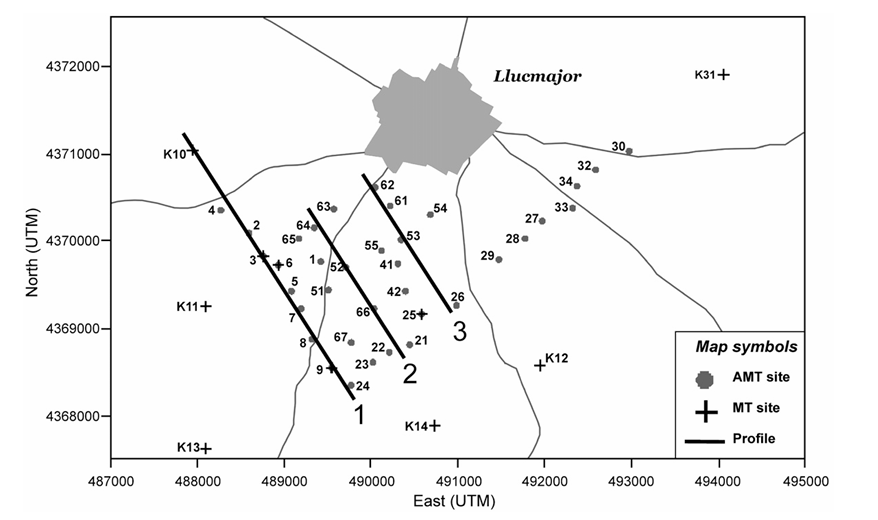
\includegraphics[width=0.75\textwidth]{Estacions Llucmajor.png}
    \caption{Mapa de la zona de Llucmajor amb les ubicacions de les estacions MT i AMT, a partir de les dades de \citet{arango2005}.}
    \label{fig:estacions}
\end{figure}

\clearpage

Per tal d'esbrinar l'origen d'aquesta aigua calenta, l'Institut Geològic i Miner d'Espanya (IGME), amb el suport del Govern Balear, va impulsar un programa d'investigació on es va plantejar un model conceptual basat en dos aqüífers superposats, un de lliure o no confinat, a la part superior, i un altre de confinat a la inferior, responsable de l'aportació d'aigua calenta, la comunicació dels quals requeriria una discontinuïtat en l'aquitard intermedi \citep{igme2003}. Ara bé, la cobertura quaternària de la zona no mostra cap evidència superficial d'aquestes estructures \citep{arango2005}. D’altra banda, les campanyes geofísiques prèvies, com sondeigs elèctrics verticals \citep{igme1985} i sísmica de reflexió \citep{benedicto1993}, van resultar insuficients per a caracteritzar el fenomen, ja sigui per les limitacions de penetració del corrent elèctric o per la manca de resolució adequada. Davant d'aquestes restriccions, la magnetotel·lúrica es va postular com la tècnica més apropiada per a obtenir un model que donés compte de l'anomalia tèrmica, donant lloc a la investigació de \citet{arango2005}, que precedeix el desenvolupament d’aquest treball.

\vspace{5pt}

A l’hora d’abordar el problema proposat, l’estudi mencionat es va encarregar, en primera instància, de repassar la estructura geològica de l’illa de Mallorca i en concret de la zona d'interès \cref{fig:estacions}. També es posà en marxa un anàlisi de dimensionalitat geoelèctrica \citep{weaver2000,marti2004} i es va fer ús de noves tècniques de processament de dades, permetent un anàlisi detallat del domini temps-freqüència i assegurant una menor dispersió en les dades que si s'apliqués una transformada de Fourier convencional \citep{arango2005}.

\vspace{5pt}

Tot i que el mètode MT permet investigar estructures a desenes o inclús centenars de quilòmetres de profunditat, en aquest cas només resulten d’interès les capes més superficials. Això es tradueix en un rang de freqüències relativament altes ($0.1$--$1000$~Hz), que en aquesta zona mostren una estructura 3D. Un anàlisi més específic mostra un subconjunt de freqüències amb una forta dominància bidimensional del terreny \citep{arango2005}. Aquest resultat, encara que constitueix una simplificació de les propietats reals del subsòl, va motivar l'ús d'un algorisme d'inversió 2D disponible en aquella data, automatitzant l'ajust de les dades MT i la generació dels perfils corresponents \citep{siripunvaraporn2000,pedersen2005}. 

\vspace{5pt}

No obstant això, l’aproximació bidimensional presenta un valor de RMS \footnote{El RMS (\textit{Root Mean Square} o valor quadràtic mitjà) és una mida estadística de la magnitud d'un conjunt de valors. En el context del processament de dades geofísiques, s'utilitza habitualment per quantificar l'error o la diferència residual entre les dades observades i les predites pel model.} elevat. Aquest indicador sovint no s'ha d'interpretar només com una deficiència numèrica, sinó com una evidència de la complexitat tridimensional del subsòl. Quan el model bidimensional és incapaç de reproduir satisfactòriament les dades observades a causa dels efectes d'inducció lateral, es posa de manifest que les simplificacions geomètriques del 2D són insuficients. Aquesta discrepància persistent actua com un diagnòstic que justifica la transició cap a enfocaments tridimensionals \citep{arango2005,egbert2014}. 
\vspace{5pt}

Per entendre la perspectiva que proporciona aquest treball, cal remarcar la importància del problema invers, que marca la principal diferència amb l’estudi esmentat. A diferència del problema directe, que permet calcular les observacions a partir d'un model conegut, el problema invers reconstrueix les propietats del subsòl a partir de les dades mesurades a la superfície. El problema invers planteja, de manera inherent, la no-unicitat, ja que existeixen múltiples distribucions de resistivitat que reprodueixen les mateixes respostes \citep{chavejones2012,egbert2014}. 

\vspace{5pt}

En MT, el punt de partida experimental és el registre de les fluctuacions dels camps elèctric i magnètic terrestres, a partir dels quals es calcula el tensor d'impedància, amb l'objectiu de derivar-ne la resistivitat aparent i la fase, representades en funció del període del senyal. 

\vspace{5pt}


La resistivitat aparent és un valor mitjà de la resistivitat del subsòl, obtingut a partir de la resposta combinada de diferents capes o estrats amb propietats elèctriques heterogènies, per tant, no s'ha de confondre en cap concepte amb la resistivitat real del material.

\vspace{5pt}


Des d'una perspectiva de modelització, l'objectiu de la inversió és reconstruir la distribució tridimensional de la resistivitat elèctrica al llarg del volum del subsòl estudiat. Aquesta propietat depèn estretament de les característiques litològiques, mineralògiques i hidrogeològiques del medi. En general, les formacions rocoses seques o compactes presenten valors elevats, mentre que la presència de fluids conductors, com ara aigües subterrànies salines, solucions hidrotermals o zones de falla altament alterades, redueixen dràsticament aquesta propietat \citep{chavejones2012,rosell2013}.
\vspace{5pt}

Alhora, factors com la porositat efectiva, la connectivitat de la xarxa de porus i la presència de fases minerals conductores secundàries juguen un paper determinant en la resposta del material. Per tant, en el context de la inversió magnetotel·lúrica, mapejar la distribució tridimensional de la resistivitat facilita la identificació de litologies, estructures profundes i contrastos d'interès hidrogeològic o geotècnic \citep{chavejones2012}.

\vspace{5pt}


A continuació s'exposaran els objectius que impulsen l'elaboració d'aquest projecte d'investigació i que donen peu al cos d'aquesta memòria. A l'apartat de metodologia s'indagarà en els aspectes matemàtics i lleis físiques que regeixen el mètode MT, així com en les simetries que abasta el tensor d'impedància en funció de la complexitat del terreny. També entrarem en contacte amb l'adquisició de dades i el seu processat per, posteriorment, incloure el model inicial escollit i entendre quins paràmetres actuen sobre la inversió executada a ModEM  \citep{egbert2014}. Finalment, analitzarem els resultats obtinguts i, de manera raonada, explicarem quins d'ells són els escollits per establir un model final. 

\begin{figure}[H]
    \centering
    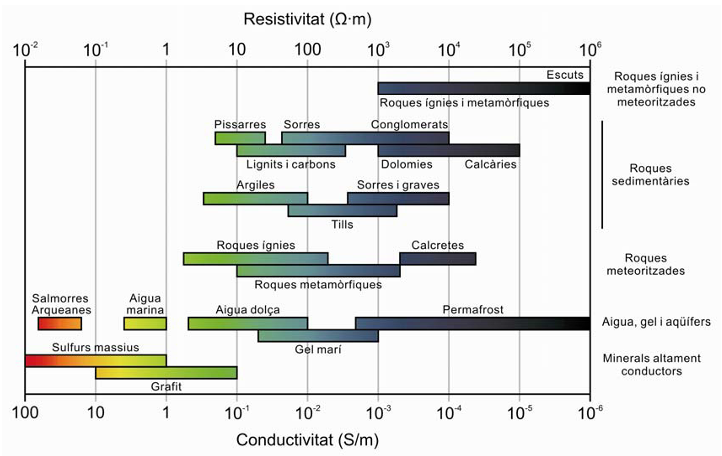
\includegraphics[width=0.60\textwidth]{resistivita geologica.png}
    \caption{Valors de resistivitat elèctrica dels materials més comuns a l’escorça terrestre, adaptats de \citet{rosell2013}.}
    \label{fig:resistivitats-materials}
\end{figure}

\subsection{Objectius}
L’objectiu principal d’aquest treball és obtenir un model 3D de la resistivitat elèctrica de la zona de Llucmajor mitjançant una inversió de dades magnetotel·lúriques sistemàtica i objectiva, utilitzant l'algorisme ModEM i els recursos del supercomputador MAGMA. Es pretén validar aquest model contrastant-lo amb els treballs previs basats en mètodes heurístics d'assaig i error \citep{arango2005}, per tal de confirmar l'origen de l'anomalia geotèrmica detectada a l'aqüífer i dotar de major rigor analític la interpretació geoelèctrica del subsòl.


\section{Metodologia}

\subsection{Fonaments del mètode magnetotel·lúric}

En aquest apartat s'introduirà de manera específica la física subjacent del mètode magnetotel·lúric, de tal manera que el lector entengui els raonaments que condueixen al desenvolupament del model.

\subsubsection{Base física i règim difusiu }

El mètode magnetotel·lúric es basa en l'estudi de les fluctuacions naturals dels camps elèctric ($\mathbf{E}$) i magnètic ($\mathbf{H}$) a la superfície terrestre, les quals indueixen corrents elèctrics a l'interior del subsòl. Aquesta interacció electromagnètica es regeix per les equacions de Maxwell [\cref{eq:faraday} i \cref{eq:ampere}] en l'aproximació quasi-estàtica \cref{eq:5}, on els corrents de desplaçament són negligibles davant dels corrents de conducció a les freqüències d'interès geofísic \citep{chavejones2012}. En un medi conductor com la Terra, el mecanisme principal de transport de càrrega sota la influència de camps electromagnètics externs són els corrents de conducció,  que poden ser produïts per fenòmens atmosfèrics, com ara bé les tormentes elèctriques, generant camps per sobre de 10$Hz$ o fenòments geomagnètics alimentats per vents solars; que produeixen camps a freqüències per sota d' 1$Hz$\citep{rosell2013}.


\begin{equation}
    \boldsymbol{\nabla} \times \mathbf{E} = -\frac{\partial \mathbf{B}}{\partial t},
    \label{eq:faraday}
\end{equation}


\begin{equation}
    \boldsymbol{\nabla} \times \mathbf{H} = \mathbf{J} + \frac{\partial \mathbf{D}}{\partial t}.
    \label{eq:ampere}
\end{equation}

 Si comparem la magnitud relativa dels corrents de conducció enfront dels corrents de desplaçament en el domini de la freqüència (amb una pulsació $\omega = 2\pi f$), la relació entre ambdós termes és:
\vspace{5pt}

\begin{equation}
    \frac{\text{Corrents de desplaçament}}{\text{Corrents de conducció}} = \frac{\omega \epsilon}{\sigma}.
    \label{eq:3}
\end{equation}

\vspace{5pt}
En el mètode MT combinat amb AMT\footnote{L'Audio-Magnetotel·lúrica (AMT) és una variant de la Magnetotel·lúrica que treballa en un rang de freqüències més elevat (típicament entre $10~\text{Hz}$ i $10.000~\text{Hz}$). Rep aquest nom perquè aquest interval de freqüències electromagnètiques coincideix amb l'espectre de les ones sonores audibles per a l'oïda humana.}, el rang de freqüències habitual d'estudi s'estén aproximadament des de $10^{-4} \, \text{Hz}$ fins a $10^3 \, \text{Hz}$ \citep{chavejones2012}. 
Per a la freqüència més alta utilitzada en aquest tipus d'estudis obtenim:
\vspace{5pt}

\begin{equation}
    \frac{\omega \epsilon}{\sigma} << 1.
    \label{eq:4}
\end{equation}

\vspace{5pt}
Sota aquesta condició, podem simplificar la 4a Llei de Maxwell suprimint el terme de la derivada temporal del camp elèctric ($\frac{\partial \mathbf{D}}{\partial t} \approx 0$), de tal manera que:

\begin{equation}
    \nabla \times \mathbf{H} \approx \mathbf{J} = \sigma \mathbf{E},
    \label{eq:5}
\end{equation}


\noindent
és a dir, el règim quasi-estàtic. Aquesta expressió, juntament amb Llei de Faraday, condueixen a dues equacions que descriuen el comportament difusiu dels camps a les freqüències mencionades, un cop penetren la superfície terrestre.
\vspace{5pt}

\begin{equation}
    \nabla^2 \mathbf{E} = \mu \sigma \frac{\partial \mathbf{E}}{\partial t},
    \label{eq:6}
\end{equation}

\begin{equation}
    \nabla^2 \mathbf{H} = \mu \sigma \frac{\partial \mathbf{H}}{\partial t}.
    \label{eq:7}
\end{equation}

\vspace{5pt}
A partir d’aquest esquema no es pot pensar en el camps electromagnètics entrants com a ones lliures en l’espai, sinó que s’han d’entendre com a fenòmens purament difusius marcats per un decaïment característic anomenat \emph{skin depth}, que posteriorment definirem \citep{weidelt1972}.

\subsubsection{El tensor d'impedància Z}

A la superfície terrestre, la relació lineal entre les components horitzontals del camp elèctric i del camp magnètic es formula a través del tensor d'impedància ($Z$), que matemàticament representa una matriu complexa de segon ordre ($2 \times 2$) expressada formalment en el domini de la freqüència mitjançant l'equació matricial \citep{weaver2000}: 

\begin{equation}
    \begin{pmatrix} E_x \\ E_y \end{pmatrix} = \begin{pmatrix} Z_{xx} & Z_{xy} \\ Z_{yx} & Z_{yy} \end{pmatrix} \begin{pmatrix} H_x \\ H_y \end{pmatrix},
    \label{eq:6}
\end{equation}


\noindent
on les components $Z_{ij}$ depenen de la freqüència i de l'estructura de resistivitat del subsòl. Són aquestes components les principals responsables d’establir la dimensionalitat del problema al que ens enfrontem i per aquest motiu cal indagar en les diferents formes que pot assolir aquest tensor.

\vspace{5pt}

El cas 1D és equivalent al d’un medi estratificat, on els diferents materials estan superposats verticalment per capes i presenten homogeneïtat horitzontal. És a dir, la resistivitat del medi només varia amb la component vertical o la fondària, per tant les components de la diagonal del tensor romanen nules. En aquest tipus de medi, les components de l'antidiagonal són iguals i de signes contraris \citep{chavejones2012,weaver2000}. 
\vspace{5pt}

\begin{equation}
    Z_{1D}(f) = \begin{pmatrix} 0 & Z(f) \\ -Z(f) & 0 \end{pmatrix}.
    \label{eq:7}
\end{equation}


\vspace{5pt}

En el cas 2D, la resistivitat varia amb la profunditat i amb una direcció horitzontal, mentre que es manté invariant al llarg de la direcció geològica preferent o \emph{strike}. Aquesta simetria es reflecteix en el tensor d'impedància \citep{weaver2000,marti2004}.
\vspace{5pt}

\begin{equation}
    Z_{2D}(f) = \begin{pmatrix} 0 & Z_E(f) \\ Z_H(f) & 0 \end{pmatrix}.
    \label{eq:8}
\end{equation}

\vspace{5pt}

Aquesta matriu representa el cas ideal on les components de l'antidiagonal presenten valors diferents i les de la diagonal són nul·les. Per obtenir aquesta forma, les components dels camps s'han d'expressar en les direccions paral·lela i perpendicular a l'\emph{strike}; quan l'orientació de mesura no hi coincideix, el tensor es pot rotar matemàticament \citep{rosell2013,marti2004}.
\vspace{5pt}. Pel que fa a la interpretació electromagnètica trobem, que per un medi 2D, $Z_E$ i $Z_H$ estan intrínsecament relacionats amb els dos modes de polarització tranversals ($T_E$ i $T_M$) en que es poden descomposar les equacions [\cref{eq:faraday} i \cref{eq:ampere}], on el primer mode defineix el camp $\mathbf{E}$ paral·lel a la direcció de l'\emph{strike}, mentre que el segon ho fa amb al camp magnètic $\mathbf{E}$, conservant sempre la propietat de perpendicularitat entre ambdós camps.

\begin{equation}
    \begin{pmatrix} Z_{xx}(f) & Z_{xy}(f) \\ Z_{yx}(f) & Z_{yy}(f) \end{pmatrix} = R_\theta \cdot \begin{pmatrix} 0 & Z_E \\ Z_H & 0 \end{pmatrix} \cdot R_\theta^T,
    \label{eq:9}
\end{equation}


\begin{equation}
    R_\theta = \begin{pmatrix} \cos\theta & \sin\theta \\ -\sin\theta & \cos\theta \end{pmatrix}.
    \label{eq:10}
\end{equation}

\vspace{5pt}

El cas més general és el principal objecte d’estudi en aquest treball. En aquesta mena de medis, les propietats elèctriques canvien en qualsevol direcció de l'espai i el tensor d'impedàncies mostra, de manera general, totes les seves components diferents de zero \citep{weaver2000,marti2004}. 
\vspace{5pt}

\begin{equation}
    Z_{3D}(f) = \begin{pmatrix} Z_{xx}(f) & Z_{xy}(f) \\ Z_{yx}(f) & Z_{yy}(f) \end{pmatrix}.
    \label{eq:11}
\end{equation}

\vspace{5pt}


En aquest estudi magnetotel·lúric 3D s'han decidit assimilar les possibles distorsions com a part de les estructures que estem analitzant, encara que es parteix d'un conjunt de dades ja processades $Z_{ij}(f)$ on s'han tractat els efectes de distorsió galvànica \citet{arango2005}.



\subsubsection{Resistivitat aparent i fase}


Un cop introduït el tensor d’impedàncies cal entendre el seu paper dintre de l’àmbit de la modelització geofísica. Les seves components complexes permeten calcular directament la resistivitat aparent i la fase \citep{chavejones2012}:
\vspace{5pt}

\begin{equation}
    \rho_{ij}(f) = \frac{1}{2\pi f \mu} \vert Z_{ij}(f) \vert^2,
    \label{eq:13}
\end{equation}


\begin{equation}
    \varphi_{ij}(f) = \arg(Z_{ij}(f)).
    \label{eq:14}
\end{equation}

\vspace{5pt}

Podem veure com la resistivitat aparent ve descrita pel determinant de la matriu de cada component del tensor en freqüència i la fase és directament l'argument d'aquest nombre complex. 

\vspace{5pt}

Cal tenir molt present que $\rho_{ij}$ no és la propietat real del subsòl que estem buscant, sinó una resposta calculada a partir de les components del tensor d’impedàncies. La resistivitat aparent i la fase representen una resposta integrada del medi, i l'objectiu de la inversió és utilitzar-les per reconstruir la distribució de la resistivitat real del subsòl \citep{chavejones2012}.

\vspace{5pt}

\subsubsection{Skin depth i profunditat d'investigació}

La profunditat de penetració o \emph{skin depth} ($\delta$) defineix la distància a la qual l'amplitud del camp electromagnètic decau fins a un factor $1/e$ (aproximadament un 37\%) del seu valor superficial \citep{chavejones2012}. Matemàticament, s'expressa com: 
\vspace{5pt}


\begin{equation}
    \delta = \sqrt{\frac{2}{\omega \mu_0 \sigma}} = \sqrt{\frac{\rho}{\pi f \mu_0}} \approx 503 \sqrt{\rho T},
    \label{eq:15}
\end{equation}

\vspace{5pt}

\noindent
on $\rho$ és la resistivitat, $T$ el període i el coeficient 503 amb unitats de metres. Val la pena tenir en compte un detall físic clau a l'hora de definir com penetra aquesta informació al subsòl. En el nostre cas particular es volen caracteritzar estructures molt superficials en comparació a la potència de penetració que presenta el mètode MT. Per això s’utilitza un rang de freqüències de treball suficientment elevades (1000-0.1)Hz com per encapçalar el sistema aqüífer de Llucmajor i optar per la millor resolució de la zona.

\vspace{5pt}

La freqüència no és l'única variable rellevant, ja que la resistivitat també influeix en la profunditat de penetració. Com que aquest valor és desconegut abans de desenvolupar el model, s’utilitza un rang de freqüències de banda ampla per cobrir les profunditats d'interès \citep{chavejones2012}.




\subsection{Dades i adquisició}

\subsubsection{Adquisició}

En la campanya duta a terme durant l'estiu de l'any 2002 es van recopilar les dades de 42 estacions, de les quals 36 utilitzaven l'instrument de mesura ADU06 (AMT) i 6 d'ells l'instrument MMS03E (MT); en 4 localitzacions es varen emprar ambdós sistemes per verificar-ne la compatibilitat. Per al modelatge tridimensional s'utilitzen 40 estacions, després d'excloure les estacions 42 i 61 \citep{arango2005}.

\vspace{5pt}

L'equip de mesura ADU06 possibilita la gravació dels camps elèctric i magnètic a través de cinc freqüències de mostratge diferents, alhora que la unitat MMS03E en fa servir tres. Tots dos sistemes incorporen un nivell addicional mitjançant el processament digital i el remostreig de la banda corresponent als intervals més lents \citep{arango2005}. 

\vspace{5pt}

El dispositiu experimental es va desplegar a partir d’un anàlisi geològic previ, seguint les orientacions presumptes del \emph{strike} NE--SW i NW--SE i projectant una malla amb una separació aproximada de 300~m \citep{arango2005}. Les correccions analítiques aplicades durant el processament permeten compensar la desalineació respecte dels eixos geoelèctrics principals \citep{marti2004,arango2005}.

\subsubsection{Processat}

Prèviament al nucli d'aquest treball, l'adquisició i el tractament de camp requereixen un flux de processament, que consisteix principalment en fer una conversió de les mesures del domini temperal al domini de les freqüències. A més a més,  considera l'estacionarietat de la font natural externa i la resposta instrumental dels equips, registrats en diferents intervals de mostratge i remostreig digital. Aquest apartat va ser ejecutat per \citet{arango2005} en la seva totalitat.

\vspace{5pt}

Per abordar l'anàlisi de les sèries temporals obtingudes en camp, el preprocessament aplica funcions de finestra, com ara la finestra de Hanning, per reduir els efectes de truncament i la fuita espectral. Posteriorment, es realitza la transformació al domini de les freqüències mitjançant decimació en cascada i la Transformada Discreta de Fourier (DFT).

\vspace{5pt}

Tanmateix, les tècniques basades estrictament en la Transformada de Fourier presenten una resolució temporal limitada, cosa que dificulta discriminar segments de baixa qualitat. Per superar aquesta limitació, el processament previ va emprar la Transformada Ondicular, que aporta localització conjunta en temps i freqüència i millora l'estimació del tensor d'impedàncies .

\subsubsection{Postprocessat}

Un cop superades aquestes etapes prèvies, el present TFG s'incorpora al flux de treball a partir de les dades del tensor d'impedàncies ja processades i convertides en 40 fitxers EDI.

\vspace{5pt}

Cada fitxer conté les parts real i imaginària de les quatre components del tensor d’impedància, les components del \emph{tipper} $T_x$ i $T_y$ i les variàncies corresponents. 

\vspace{5pt}

L'\autoref{annex:fitxer-edi} mostra, com a exemple, el fitxer EDI complet
corresponent a l'estació 01.

\vspace{5pt}


Alhora, cada part mencionada és un vector de la mateixa mida que el nombre total de freqüències mesurades, variant en funció de cada estació. 
Tant en aquest estudi com a l’anterior \citep{arango2005} no s’ha tingut en compte el Tipper. Més enllà d’aportar informació addicional per a estructures 3D, la qualitat de les dades no ha permès obtenir-ne resultats concloents.

\vspace{5pt}

Encara que el processat aconsegueix sense cap mena de dubte una qualitat satisfactòria de les dades, és precís fer un depurat manual a posteriori de la resistivitat aparent i la fase, per evitar que l’algorisme d’inversió consumeixi potència de càlcul innecessària tractant d’ajustar unes dades que es desvien clarament de la tendència principal i que manquen de sentit físic. Aquest raonament ve determinat per 3 conceptes principals:
\vspace{5pt}

\begin{enumerate}
    \item \textbf{Relació lineal i causalitat \citep{chavejones2012}:} La impedància actua com una connexió directa i lineal entre el camp elèctric i el magnètic de la Terra. En tractar-se d'un sistema lineal i causal, la resposta correspon a una funció holomorfa i analítica en el domini de la freqüència, la qual cosa exigeix que aquesta funció sigui estrictament suau i contínua.

    \item \textbf{Relacions de Kramers-Kronig i coherència de dades \citep{fischerschnegg1980}:} Gràcies a les relacions de Kramers-Kronig, la part real i la imaginària de la impedància no són independents, sinó que estan estretament lligades per la causalitat. En magnetotel·lúrica, això es tradueix en el fet que la fase depèn directament del pendent de la corba de resistivitat aparent en escala logarítmica respecte al període. Aquest vincle matemàtic obliga que tota la informació variï de manera coherent i gradual; la presència de salts o esglaons artificials en la resistivitat aparent implicaria un comportament de la fase mancat de sentit físic.

    \item \textbf{Naturalesa difusiva dels camps \citep{weidelt1972}:} Finalment, cal considerar la naturalesa purament difusiva dels camps electromagnètics a l'interior de la Terra. A les freqüències d'interès magnetotel·lúric, el camp no es propaga com una ona electromagnètica ràpida, sinó que es difon de manera gradual sota un règim quasi-estàtic governat per l'equació de difusió, on s'ignoren els corrents de desplaçament.

A les figures 3 i 4 que es mostren a continuació i trobem la comparació entre les dades originals i les depurades manualment, per les expressions $\log_{10}(\rho_a)$ vs $\log_{10}(T)$:
\end{enumerate} 


\begin{figure}[H]
    \centering
    \begin{minipage}[t]{0.49\textwidth}%
        \centering
        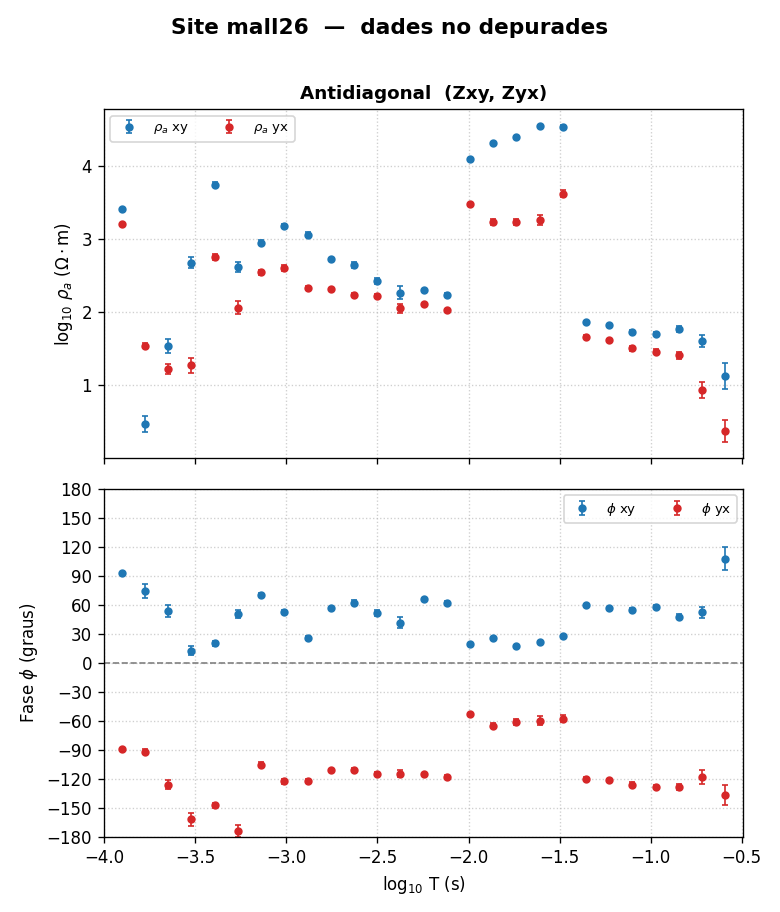
\includegraphics[width=\linewidth]{mall26_no_dep.png}%
    \end{minipage}%
    \hfill
    \begin{minipage}[t]{0.49\textwidth}%
        \centering
        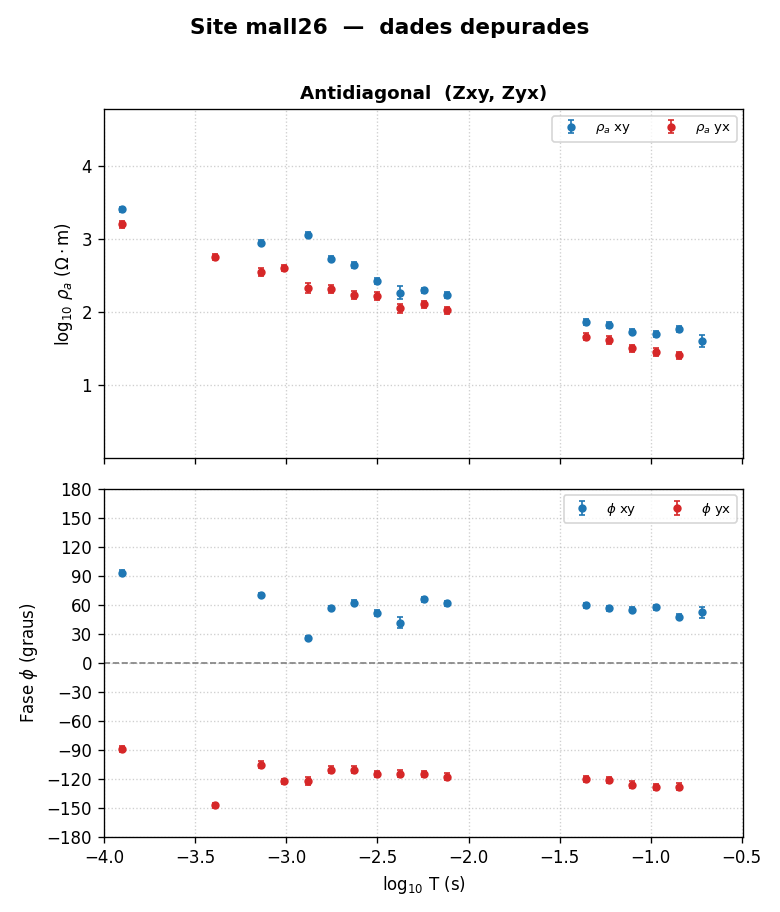
\includegraphics[width=\linewidth]{mall26_dep.png}%
    \end{minipage}
    \caption{Comparativa de l'estació 26 entre les dades processades per \citep{arango2005} i el postprocessat realitzat manualment.}
    \label{fig:comparacio-depuracio-26}
\end{figure}

\begin{figure}[H]
    \centering
    \begin{minipage}[t]{0.24\textwidth}%
        \centering
        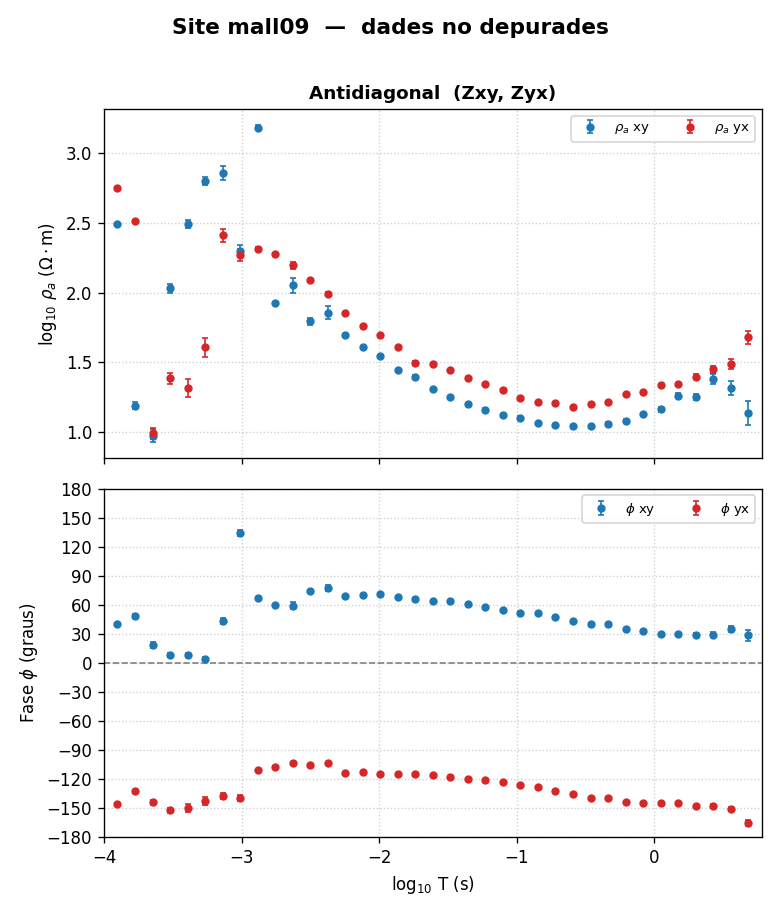
\includegraphics[width=\linewidth]{mall09_no_dep.png}\par
        \scriptsize Estació 10\\original
    \end{minipage}%
    \hfill
    \begin{minipage}[t]{0.24\textwidth}%
        \centering
        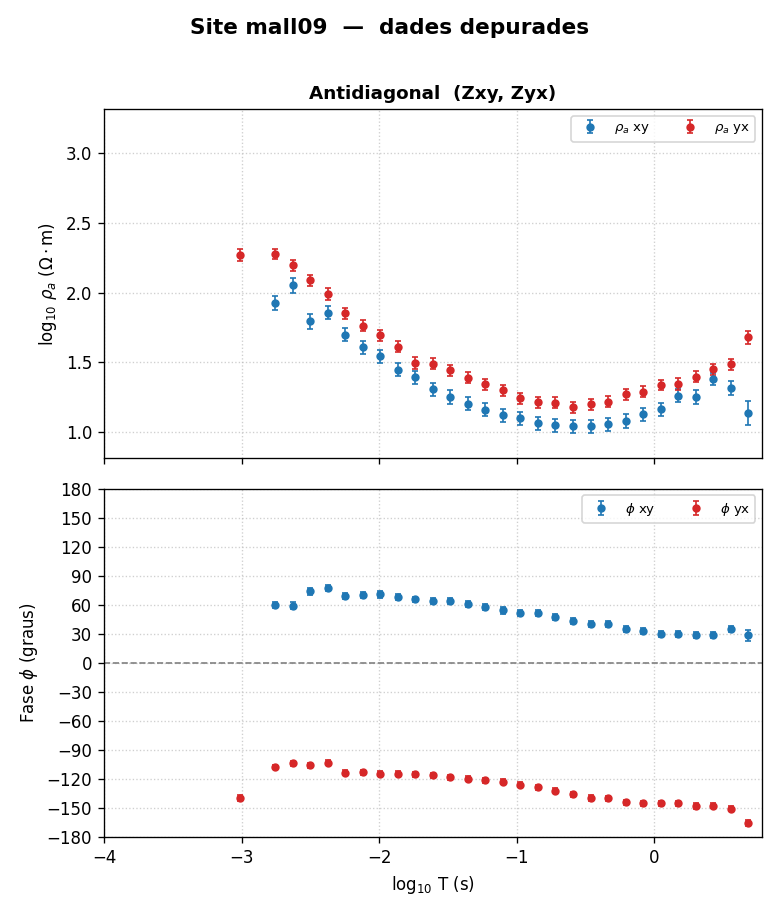
\includegraphics[width=\linewidth]{mall09_dep.png}\par
        \scriptsize Estació 10\\depurada
    \end{minipage}%
    \hfill
    \begin{minipage}[t]{0.24\textwidth}%
        \centering
        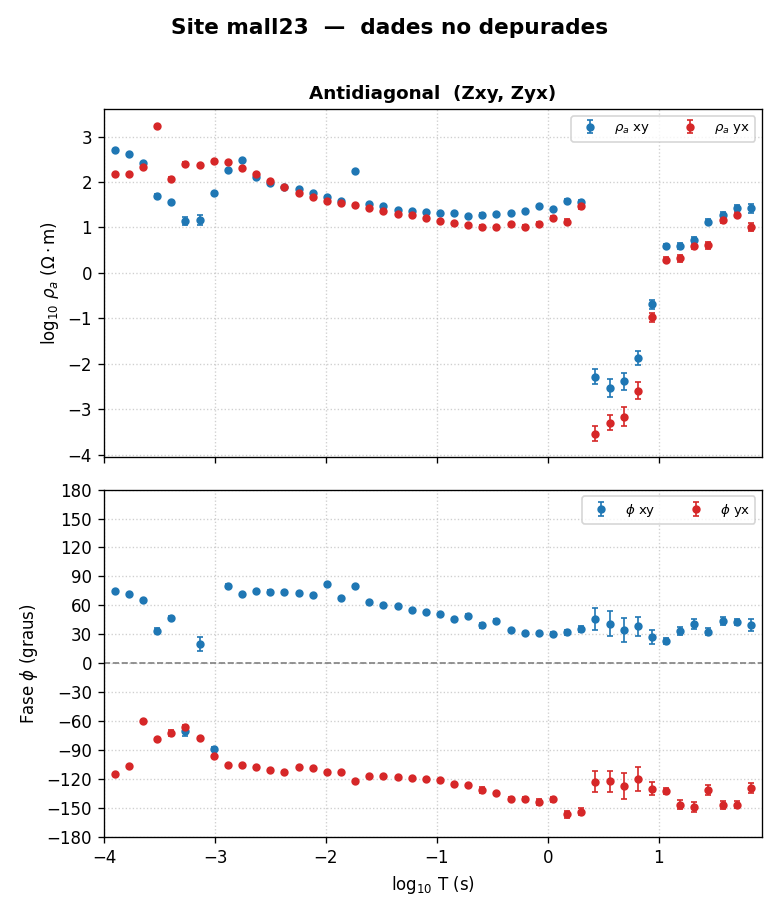
\includegraphics[width=\linewidth]{mall23_no_dep.png}\par
        \scriptsize Estació 23\\original
    \end{minipage}%
    \hfill
    \begin{minipage}[t]{0.24\textwidth}%
        \centering
        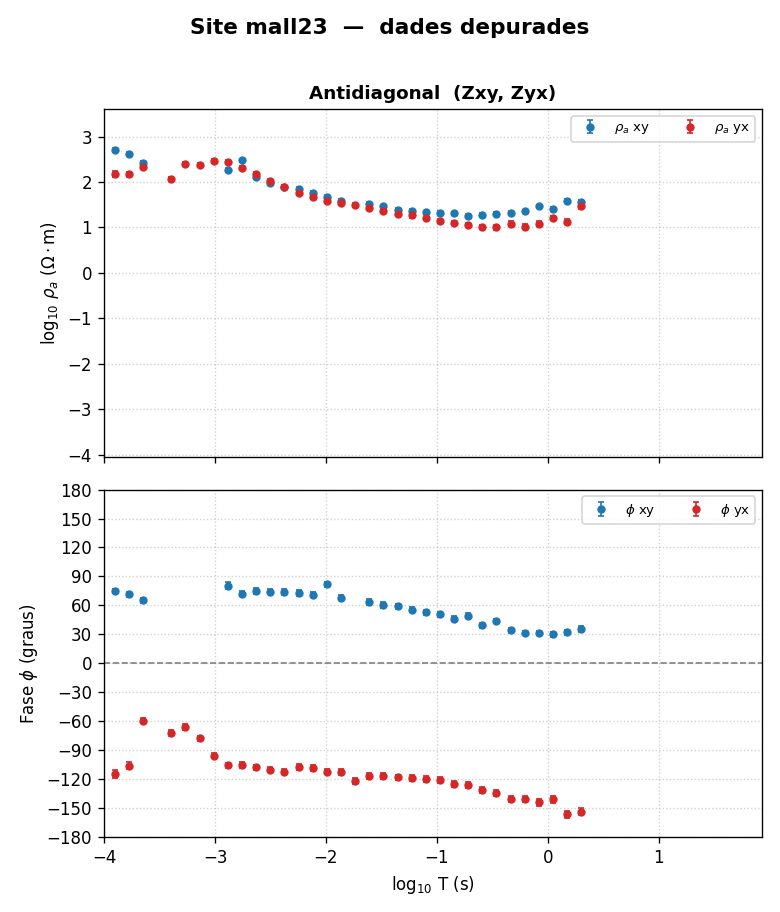
\includegraphics[width=\linewidth]{mall23_dep.png}\par
        \scriptsize Estació 23\\depurada
    \end{minipage}
    \caption{Comparativa de l'estació 9 i 23 entre les dades processades per \citep{arango2005} i el postprocessat realitzat manualment.}
    \label{fig:comparacio-depuracio-10-23}
\end{figure}

\vspace{5pt}

Aquest depurat s’ha intentat automatitzar sense èxit mitjançant codis de suavitzat, aplicant mètodes com el filtre de Hampel \citep{hampel1974,davies1993} o LOWESS \citep{cleveland1979}. S’ha demostrat empíricament que cap dels dos aporta rigor suficient al model, sempre i quan s’utilitzin per filtrar una mostra d’alta dispersió, com és el cas d’alguns dels nostres fitxers. Dit d’una altra manera, els algorismes mencionats es dediquen a construir una tendència a partir dels punts veïns i, depenent dels paràmetres escollits, s’eliminen aquelles dades que presenten desviacions. Ara bé, si el renou és elevat s’acaba contaminant aquesta tendència i el filtrat proporciona resultats que no representen la realitat geofísica. Per aquest motiu un filtrat a mà juntament amb coneixements previs sobre el tractament de dades MT és l'opció que ofereix una major qualitat de dades.

\subsection{Modelització i Inversió}


Els següents apartats fan referència a la part més pràctica d'aquest treball, començant per la descripció i representació model inicial de resistivitats, així com l'especifició de les característiques de la malla on s'ejecutarà el problema invers de manera iterativa. Seguidament s'indagarà en els fonaments matemàtics de l'algorisme NLCG, per tal d'entendre el funcionament intern del problema invers i determinar l'orientació del flux de treball exposat en l'ultim apartat d'aquesta secció. 


PARAGRAF INTRODUCTORI: MODEL INI. - RESPOSTES - PROB. DIRECTE - MINIMITZAR DIFERENCIES AMB DADES (INVERSIO/AJUST)  - FLUX DE TREBALL
(POTSER CAL EXPLICAR FUNCIONAMENT MODEM)

\subsubsection{Model inicial}

El software utilitzat requereix de dos inputs essencials que marquen la principal diferència en la obtenció i posterior interpretació de resultats. Per una banda tenim el fitxer de dades, que inclou les components del tensor d’impedància i que servirà per anar comparant iterativament el model fins convergir de la manera més aproximada possible a les mesures. D’altra banda tenim el model inicial, que s’utilitzarà com a punt de partida en la inversió. Aquest fitxer conté un valor de resistivitat per a cada punt de la malla i s’ha d’ajustar a les dimensions adequades per complir les condicions de contorn establertes pel mètode MT \citep{chavejones2012}.


\vspace{5pt}


El model inicial i la regularització condicionen el punt de partida i l'estabilitat de la inversió. Tanmateix, introduir-hi un excés d'estructures pot esbiaixar el resultat; per això s'ha optat per un model de referència senzill que permeti a les dades controlar l'estructura recuperada \citep{egbert2014}.

\vspace{5pt}


\begin{figure}[H]
    \centering
    \begin{minipage}[c]{0.56\textwidth}
        \centering
        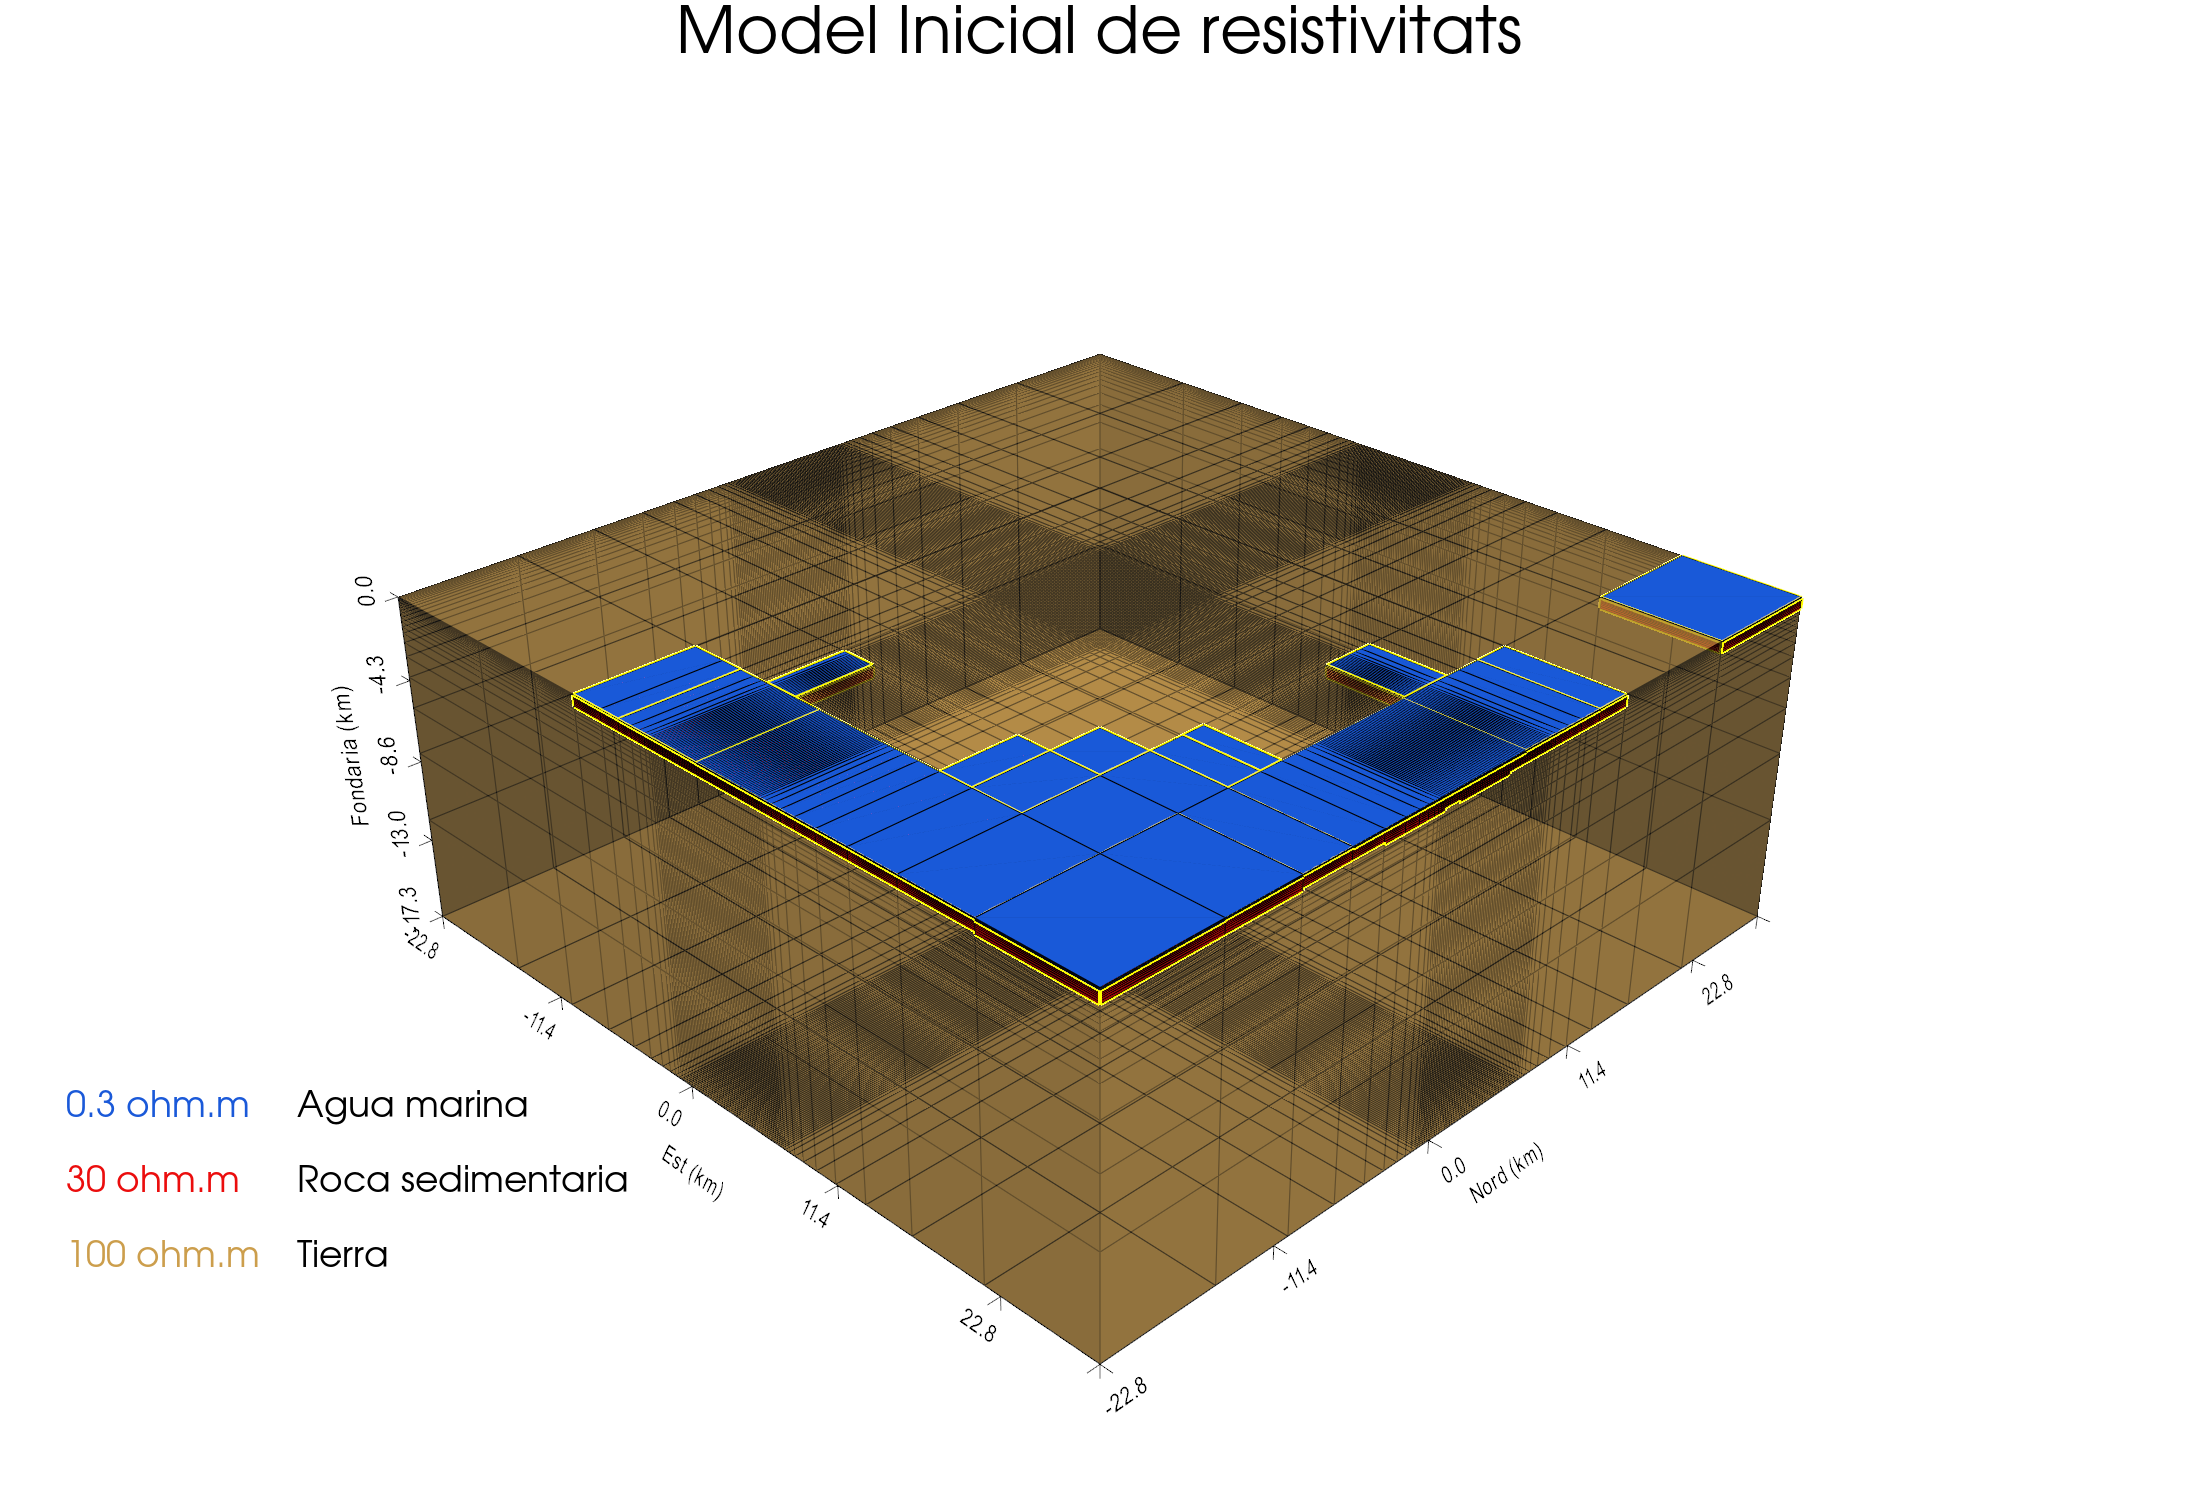
\includegraphics[width=\linewidth]{model_3D.png}\par
        \small Vista tridimensional
    \end{minipage}\hfill
    \begin{minipage}[c]{0.40\textwidth}
        \centering
        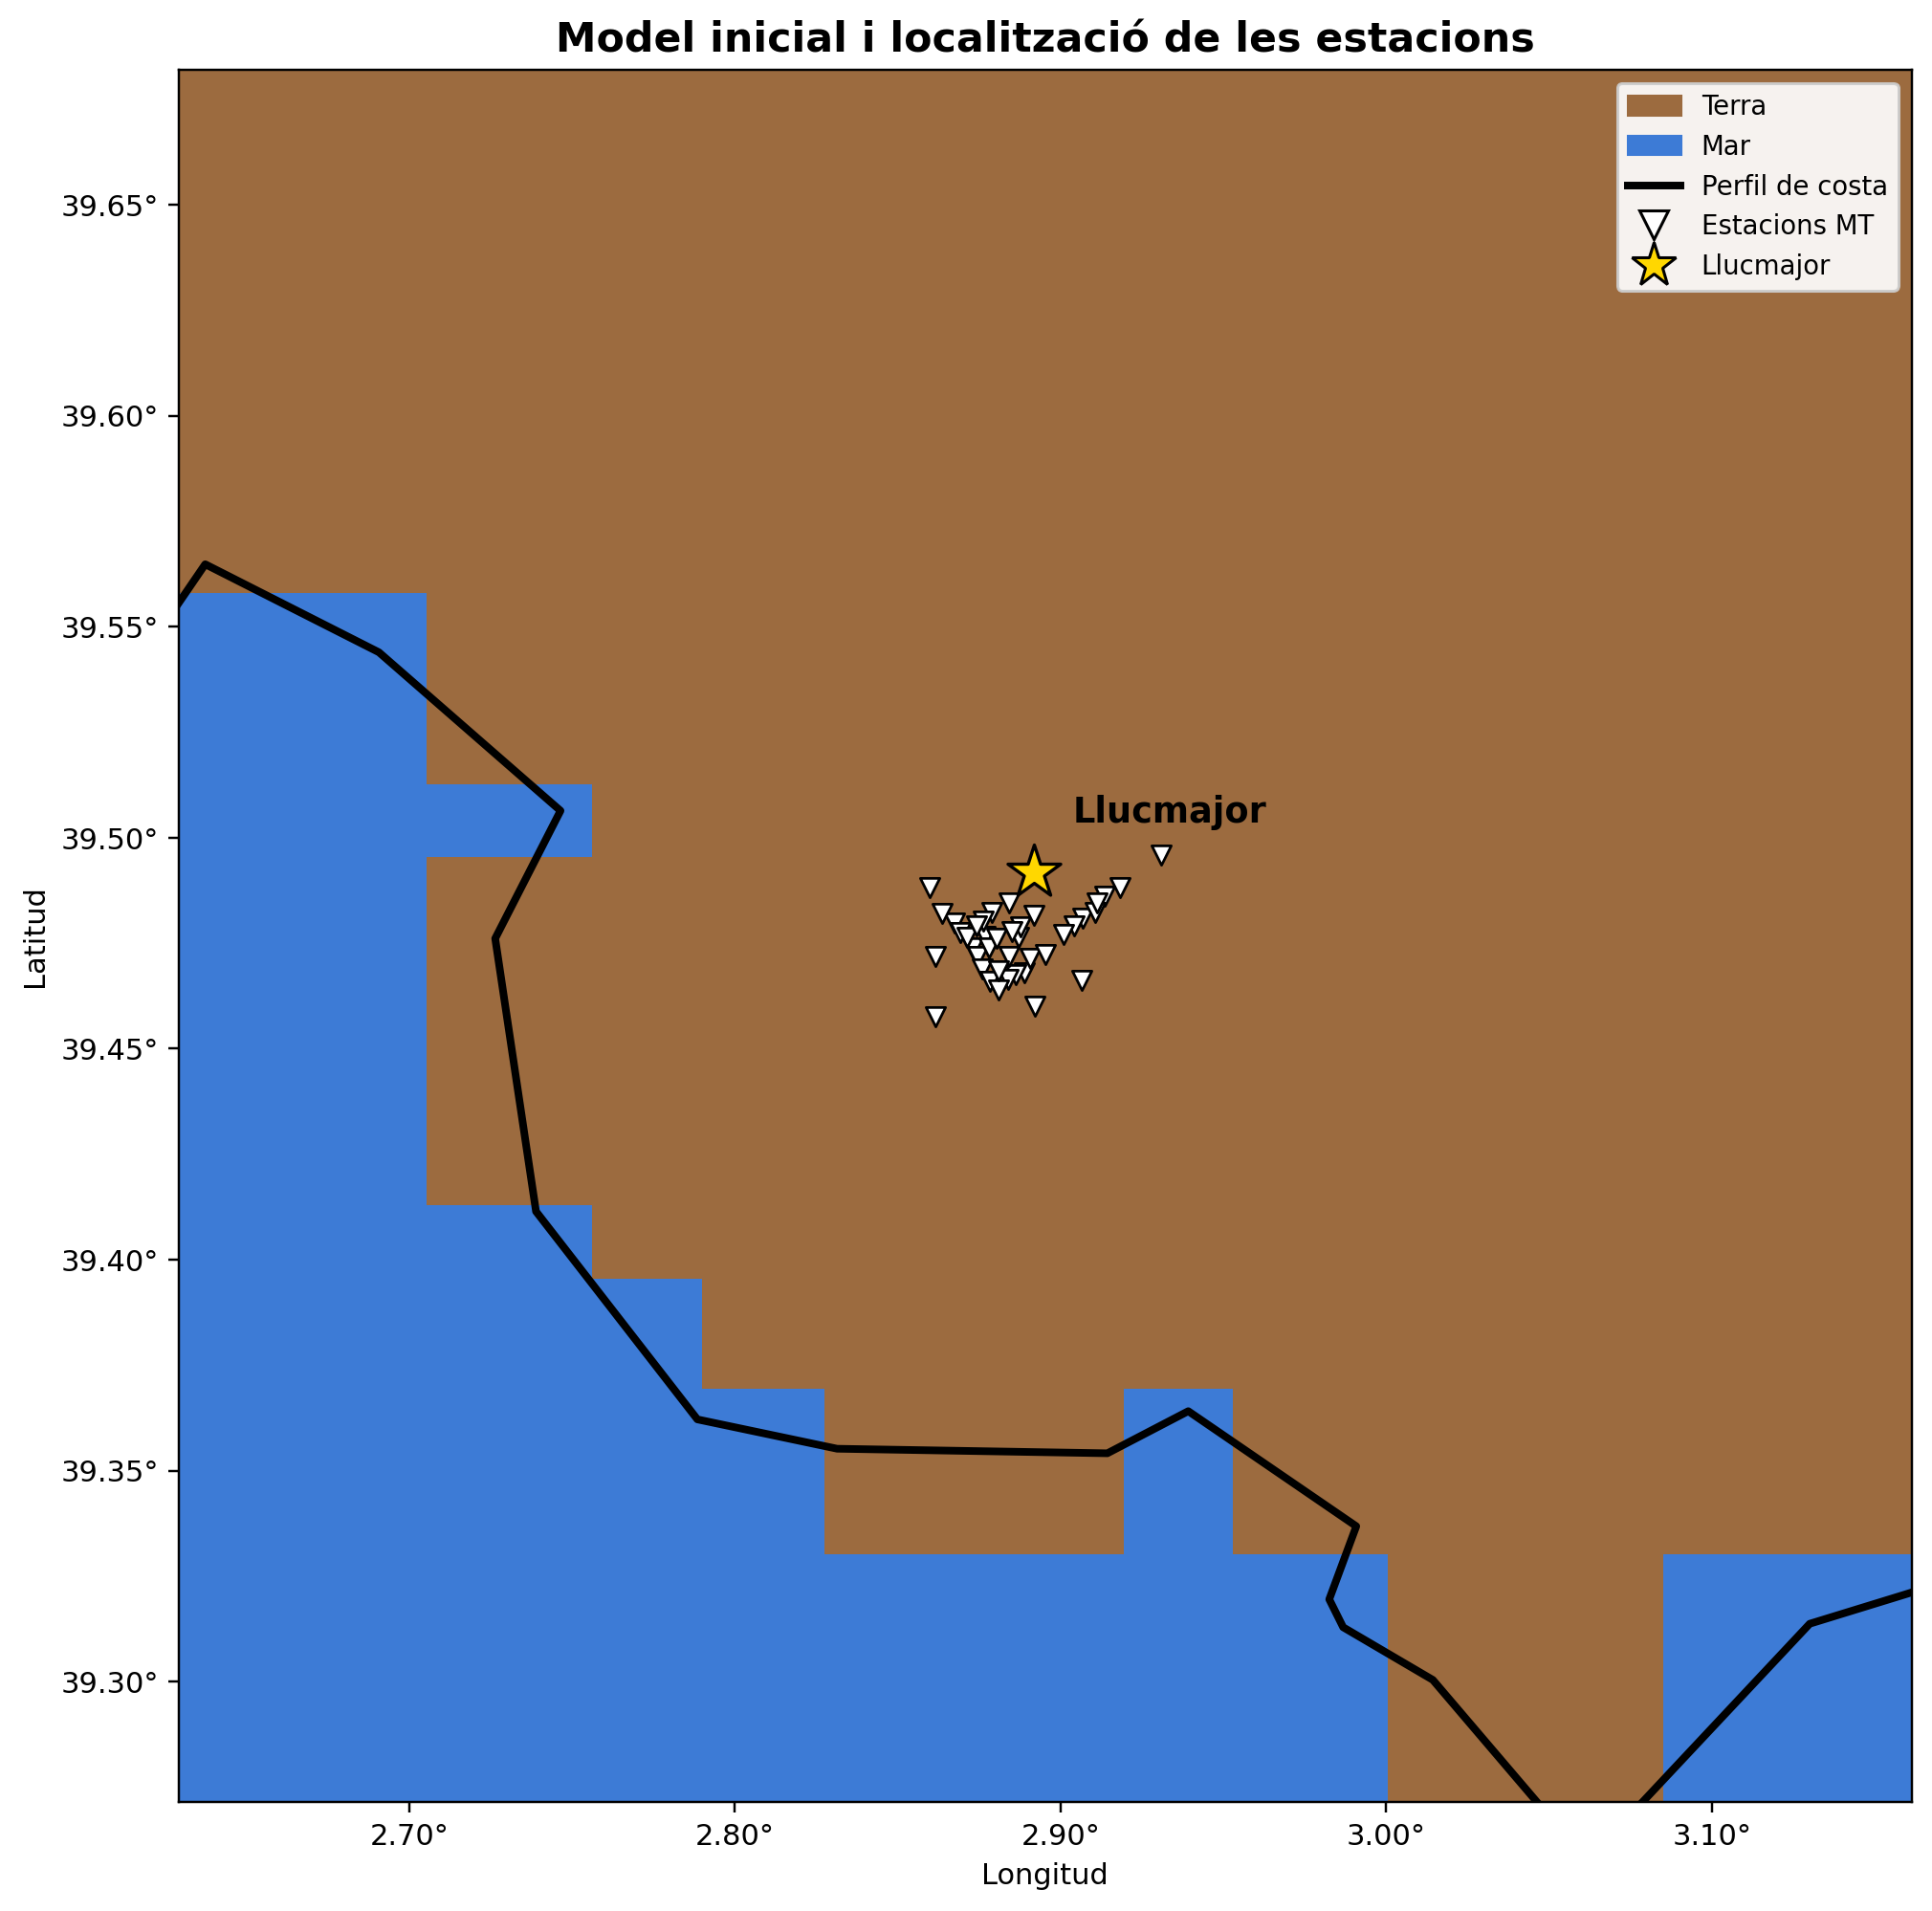
\includegraphics[width=\linewidth]{model_inicial_planta_2d.png}\par
        \small Vista en planta
    \end{minipage}
    \caption{Model resistiu inicial en vista tridimensional (esquerra) i en planta (dreta). La vista tridimensional inclou les tres resistivitats inicials (mar, terra i roca sedimentària), aplicant un valor immutable de 0.3 $\Omega \cdot m$ a la massa marina. La vista en planta mostra el perfil geogràfic utilitzat per generar el límit de costa.}
    \label{fig:model-inicial}
\end{figure}



\vspace{5pt}

El programa utilitzat per la generació d’aquest model és el 3D Grid \citep{meqbel2006}. Per adoptar un model inicial d’acord amb la geografia de la zona i que sigui compatible amb les condicions de contorn s’han tingut en compte els següents paràmetres:

\begin{table}[H]
\centering
\small
\begin{tabular}{@{}ll@{}}
\toprule
\textbf{Paràmetre} & \textbf{Valor} \\
\midrule
Cel·les totals (X\,$\times$\,Y\,$\times$\,Z) & $82 \times 82 \times 27$ \\
\midrule
\multicolumn{2}{@{}l}{\textit{Direcció X}} \\
Nombre de cel·les (nucli) & 62 \\
Dimensió de cel·la & 115 m \\
Cel·les de padding (per costat) & 10 \\
Factor de creixement (padding) & 1,5 \\
\midrule
\multicolumn{2}{@{}l}{\textit{Direcció Y}} \\
Nombre de cel·les (nucli) & 62 \\
Dimensió de cel·la & 115 m \\
Cel·les de padding (per costat) & 10 \\
Factor de creixement (padding) & 1,5 \\
\midrule
\multicolumn{2}{@{}l}{\textit{Direcció Z}} \\
Nombre de capes & 27 \\
Gruix de la primera capa & 10 m \\
Factor de creixement (zona fina) & 1,2 \\
Factor de creixement (padding profund) & 1,5 \\
Profunditat total del domini & $17{,}28$ km \\
\bottomrule
\end{tabular}
\caption{Paràmetres de la malla del model inicial.}
\label{tab:1}
\end{table}

\vspace{5pt}


A la pràctica, els codis de diferències finites fixen els valors de contorn a partir d'una solució de referència en les cares del domini. Perquè aquesta aproximació sigui vàlida, el camp anòmal generat per les heterogeneïtats laterals ha d'haver decaigut de manera negligible en arribar al marge del model, d'acord amb el comportament difusiu $\vert E(z)\vert = E_0 e^{-z/\delta}$ \citep{chavejones2012,egbert2014}.

\vspace{5pt}

A partir d'aquesta base física, el domini de \emph{padding} s'estén diverses profunditats de penetració respecte de la zona d'interès, de manera que el camp anòmal sigui prou petit als contorns i aquests no interfereixin artificialment en la resposta \citep{chavejones2012,egbert2014}.
\vspace{5pt}

En treballs previs a la regió s'havia optat per descartar l'efecte de costa \citep{arango2005}, sota la premissa que la distància a la mar feia negligible la seva influència en el rang de freqüències analitzat \citep{pous1995}.

\vspace{5pt}

No obstant això, en el marc d'aquest treball s'ha adoptat una aproximació més realista i robusta: s'ha decidit incloure explícitament la costa dins del domini de modelat 3D. Gràcies a la capacitat de càlcul de ModEM i a la potència de càlcul del supercomputador MAGMA, s'ha pogut assumir la complexitat lateral que suposa la interfície terra-mar, evitant simplificacions i permetent que la inversió resolgui de manera natural els contrastos de resistivitat. 

\vspace{5pt}

Mentre l'efecte de costa sí s'ha decidit incluir en la memòria, la topografía s'ha considerat totalment plana en aquest model ja que les variacions topogràfiques presentades pel sistema aqüífer de Llucmajor són ínfimes. 


\subsubsection{Inversió amb ModEM}

La modelització i inversió d'aquest estudi s'ha dut a terme mitjançant ModEM \citep{egbert2014}, un sistema modular d'inversió electromagnètica 3D que s'ha configurat específicament per processar dades de magnetotel·lúrica 3D utilitzant el tensor d'impedància complet a través de l'algorisme de gradient conjugat no lineal (NLCG). El fil conductor de tota aquesta secció metodològica s'expressa a través de la funció de cost:

\vspace{5pt}

\begin{equation}
    \Phi(m,d) = (d-f(m))^T C_d^{-1} (d-f(m)) + \nu (m-m_0)^T C_m^{-1} (m-m_0),
    \label{eq:16}
\end{equation}


\vspace{5pt}


\noindent
el terme de dades $d$ es compara amb la resposta del model directe $f(m)$ ponderat per la matriu inversa de la covariància de les dades $C_d$, la qual s'alimenta directament dels errors expressats en termes de variància $\sigma^2$

\vspace{5pt}

Alhora, el terme de regularització s'estructura mitjançant el model inicial $m_0$ i la matriu de covariància del model $C_m$ (que inclou els paràmetres de suavitzat i la màscara del mar), mentre que el paràmetre $\lambda$ regula el pes relatiu entre l'ajust de les dades i l'estabilitat del model.
\vspace{5pt}

Per resoldre el problema directe, ModEM discretitza les equacions de Maxwell en règim quasi-estàtic \cref{eq:4},\cref{eq:5} mitjançant diferències finites i resol els sistemes lineals resultants amb procediments iteratius i precondicionament \citep{egbert2014}.
\vspace{5pt}

Pel que fa a la regularització i la gestió de l'espai de models, s'ha aplicat un esquema d'autoregressió recursiva descrit a la literatura de referència del codi \citep{egbert2014}, configurat amb un factor de suavitzat de 0,2 en les tres direccions espacials, aplicat en dues iteracions i integrant una màscara d'oceà on el mar es manté fix. Aquest fitxer de covariància assegura que els canvis de resistivitat entre cel·les veïnes siguin geològicament suaus, evitant variacions dràstiques artificials.
\vspace{5pt}

Per resoldre aquesta optimització matemàtica, ModEM pot emprar l'algorisme de gradients conjugats no lineals (NLCG), que calcula el gradient mitjançant l'enfocament adjunt i evita formar explícitament la matriu jacobiana completa \citep{rodi2001,egbert2014}.


\vspace{5pt}

El progrés de la inversió s'avalua mitjançant l'RMS normalitzat, que quantifica el desajust entre la resposta del model i les observacions tenint en compte els errors assignats.

\vspace{5pt}


\begin{equation}
    \text{RMS} = \sqrt{\dfrac{1}{N} \sum_{i=1}^{N} 
    \left( \dfrac{d_i^{\text{obs}} - d_i^{\text{pred}}(\mathbf{m})} {\sigma_i} \right)^{2}},
    \label{eq:17}
\end{equation}

\noindent
on N és el nombre total de dades MT ($N= N_{estacions}\cdot N_{freqüències} \cdot N_{components}$), d_i^{\text{obs}} i d_i^{\text{pred}} són les dades individuals observades i predites per la inversió, i $\sigma_i$ l'error associat a cada dada observada. Cal matissar que l'expressió esmentada per $N$ no és exactament així un cop s'han depurat les dades ja que algunes estaciones presentaran menys freqüències a causa del filtratge.
\vspace{5pt}

\subsubsection{Flux de treball}


Per garantir una correcta interpretació dels resultats i extreure'n conclusions fermes sobre el model final, s'ha optat per seguir un flux de treball caracteritzat per modificacions singulars dels paràmetres en cada execució. Aquelles configuracions que denoten una millora respecte de l'anterior, s'han anat actualitzant i s'han establert com a punt de partida. Aquesta manera progressiva i ordenada d'executar les inversions, permet una intuïció lògica, així com un enteniment del funcionament de ModEM i un estalvi de temps a l'hora d'intentar reproduir pràctiques similars.


\vspace{5pt}

Prèviament a cada ejecució del model a invertir, s'han analitzat i estudiat manualment cadascún dels paràmetres generats per les respostes obtingudes, per tal d'assegurar l'eficàcia de la nova solució que volem calcular i optimitzar el procés general del flux de treball.

\vspace{5pt}

A continuació es mostra desglossat el flux de treball establert:


\begin{enumerate}
    \item \textbf{Raw data}: Model inicial ajustat a les condicions geogràfiques de la zona d'estudi i als períodes mesurats per garantir la validesa de les condicions de contorn. En aquest cas les dades no s'han depurat, mantenit el renou i forçant a l'algorisme a ajustar la dispersió.
   
    \item \textbf{Suavitzat LOWESS 1}: En aquest intent es depuren depurar les components antidiagonals del tensor d'impedàncies mitjançant el mètode LOWESS \citep{cleveland1979}. El model roman igual que al cas anterior.
    
    \item \textbf{Suavitzat LOWESS 2}: Mantenint les dades intactes, s'aposta per aplicar una capa de roca sedimentària d'uns 30~$\Omega\cdot\mathrm{m}$ fins a 500~m per sota del mar, a partir d'incloure les dades batimètriques de la costa mallorquina, proporcionades per EMODnet Bathymetry \citep{emodnet}.
    
    \item \textbf{Suavitzat Hampel}: Evolucionem cap a un tractament de dades més agressiu a partir d'aplicar un filtre Hampel a les components antidiagonals. El model $\m_0$ és exactament el mateix que l'anterior \citep{hampel1974,davies1993}.
    
    \item \textbf{Depuració manual 0}: Aquí es depuren manualment les dades ($Z_{xy}$, $Z_{yx}$) que es desvien de la tendència principal, deixant intactes les components de l'antidiagonal. Aquesta pràctica segueix més de prop les directrius de l'estudi de referència \citep{arango2005}.
    
    \item \textbf{Depuració manual (0 + ef 5)}: Aquest cas és el mateix que l'anterior, excepte per l'aplicació d'un \emph{error floor}\footnote{L'\emph{error floor} (o sòl d'error) és un llindar mínim assignat a la incertesa de les dades per evitar que observacions amb errors nominals molt petits dominin excessivament la inversió. Si  $ef = 5\%$  l'error de cada component ha de complir $\sigma_{ef} \ge \text{ef} \cdot \sqrt{\vert Z_{xy} Z_{yx} \vert}$} del 5\% a totes les components del tensor d'impedàncies.

    \item \textbf{Depuració manual 1}: En aquest cas s'acoten els períodes als 10s tal i com proposa \citep{arango2005}, amb un floor del 5\% a totes les components igual que abans, mantenint un rang de freqüències suficientment ampli com per estudiar amb bona resolució la zona d'interès.

    
    \item \textbf{Depuració manual 2}: Agafant el mateix rang de freqüències, es depuren també les components de la diagonal a l'hora que se'ls hi aplica un floor del 7\% degut a la seva alta dispersió.
    
    \item \textbf{Depuració manual 3}: En aquesta passa es decideix restringir el rang de períodes a 1s amb un error floor global del 5\%.

    \item \textbf{Depuració manual 4}: Finalment, a partir d'un estudi individual de les estacions, s'opta per agafar el resultat anterior depurant lleugerament les components diagonals més sorolloses.    

\end{enumerate} 


\section{Resultats}

\subsection{Convergència del problema invers}


Abans d'entrar en l'avaluació detallada de l'estructura geoelèctrica del subsòl,
resulta fonamental analitzar el comportament de la inversió des d'una perspectiva
global, posant el focus en la relació entre el grau de desajust de les dades, la
regularització aplicada i la complexitat estructural.
Durant el procés de resolució del problema invers
implementat a ModEM, s'han contrastat diverses estratègies de tractament de dades i
paràmetres de control, com ara la composició resistiva del model inicial, l'ús de diferents filtres de suavitzat enfront de
depuracions manuals selectives i l'aplicació d'errors, amb l'objectiu de trobar un equilibri òptim que eviti
tant el sobreajust del soroll instrumental com la pèrdua d'informació tridimensional
clau. En aquest context, l'estudi comparatiu no es pot limitar únicament a la
minimització numèrica de l'RMS, sinó que requereix una interpretació conjunta de la
norma del model (formalment expressat com $\|\mathbf{m}\|^2$ però que per simplificar l'anomeraem $m^2$), de la influència dels errors assignats i de la coherència geològica
de les estructures recuperades, establint així les bases metodològiques que
justifiquen l'elecció del model final presentat en aquest treball.


\vspace{5pt}

En l'evolució del RMS (\cref{fig:rms-convergencia}) s'aprecien clarament dues famílies de models. Primerament trobem les
inversions [dades \emph{raw} i Depuració Manual 0 (DM 0)], a més a més dels models LOWESS 1/2 i Hampel que es presenten a l'apèndix~\ref{annex:grafs-suavitzats} per mantenir una visualització nítida dels resultats principals.
Aquest conjunt aboca un RMS que arrenca al voltant dels $ 48$ punts i s'estanca entre els $13$ i els
$14$. Encara que el model inicial es refina en la transició del LOWESS~1 al~2, aquest canvi tan sols permet invertir lleugerament més potència de càlcul a ajustar les dades i constitueix una variació poc representativa de desajust.

\vspace{5pt}

 Clarament, les depuracions manuals, que inclouen l'\emph{error floor}, aconsegueixen aproximar-se més a les observacions, començant amb  un $\text{RMS}$ molt més baix
($\approx 9\text{–}11$) i descendint fins a valors de $3\text{–}7$, respaldant l'argument descrit per \citet{egbert2014}, on manifesta que l'utilització de l'error floor entre el 5\% i el 10\% evita que la inversió divergeixi o creï artefactes deguts al soroll o a la resolució de la xarxa. Una de les apreciacions més destacables és la poca capacitat de continuar iterant per part dels models DM 0 i DM 0 + ef. En aquests dos casos no s'han acotat els períodes, és a dir, la fondària de la malla és major que la dels altres models (87km), això sumat a que el nombre de dades s'han reduït significativament degut a la depuració, es pot traduir com una falta d'informació per continuar generant estructura. De fet, aquestes iteracions es van cancel·lar a mà ja que l'execució es va estancar a l'iteració 23 en ambdós exemplars. Com es pot veure a la Figura~\ref{fig:lambda-norma} el paràmetre de decaïment $\lambda$ no arriba al seu límit.


\begin{figure}[H]
    \centering
    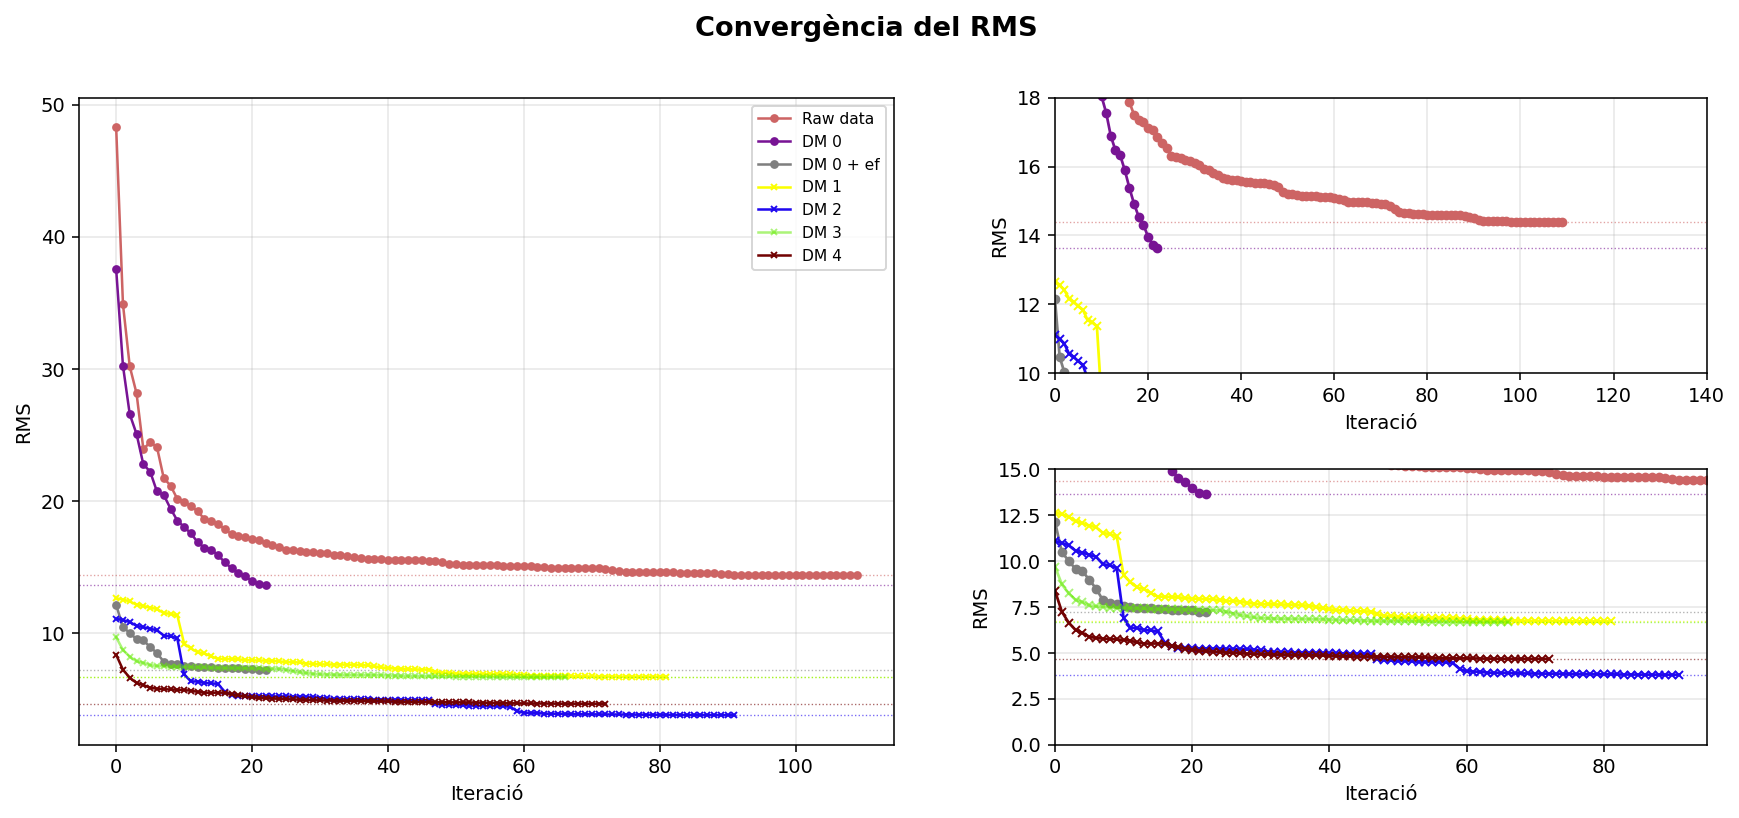
\includegraphics[width=0.9\textwidth]{rms_comparison_base.png}
    \caption{RMS en funció del nombre d'iteracions generades per ModEM. S'observa l'evolució de l'ajust per cada conjunt de dades utilitzat i model inicial. A la dreta es representa una visió amplida de la gràfica per una millor apreciació dels resultats. Finalment les sigles DM corresponen al procés de 'Depuració Manual'. }
    \label{fig:rms-convergencia}
\end{figure}

Una altra millora significativa que mereix mencionar-se és el repunt en la convergència del RMS que es genera en els models Raw Data, LOWESS 1/2 i Hampel (\cref{fig:lambda-norma} i Apèndix \ref{annex:grafs-suavitzats}) i que distingeix clarament el mètode de depuració manual dels altres casos, eliminant per complet aquesta tendència abrupta que genera una reversió en l'ajust i que produeix estructura artificialment (mirar iteració 7 en le gràfiques de $m^2$ (\cref{fig:lambda-norma}) i Apèndix \ref{annex:grafs-suavitzats}).
\vspace{5pt}

Cal tenir present que el valor de l'RMS no es pot comparar directament entre
models amb un nombre de dades $N$ o uns errors $\sigma_i$ diferents. Si s'eliminen dades o s'inflen els errors, l'RMS disminueix per construcció sense
que això impliqui necessàriament un model físic millor. Per això, s'ha d'analitzar
sempre conjuntament amb $m^2$ (la norma del model respecte a $m_0$) i $\lambda$ (la
regularització, que acaba al límit de $10^{-8}$ abans que es produeixi la sortida
automàtica o \emph{auto-exit}).

\vspace{5pt}

Dins de les estratègies, la DM 3 i 4 presenten un paràmetre de regularització que descendeix amb més facilitat (\cref{fig:lambda-norma}) (esquerra), l'algorisme resol millor el problema a cada escala abans d'introduir
detall, l'estructura es construeix de manera coherent i són les que més complexitat
conserven dins de les que tenen error floor aplicat ($m^2 \approx 0{,}41$). 

\vspace{5pt}
En contrast, la Depuració Manual~2 actua sobre la diagonal 
($Z_{xx}$, $Z_{yy}$). Com que aquestes components són petites,
sorolloses i contenen informació relacionada amb els efectes 3D \citep{weaver2000,groom1991}; treure-les simplifica el conjunt i
fa caure l'RMS fins a $3{,}81$. El problema és que s'elimina la informació 3D
essencial, provocant que la inversió perdi resolució i el model es suavitzi en excés
($m^2 \approx 0{,}15$). Es tracta d'un RMS en bona part cosmètic, on es guanya en ajust numèric a costa de perdre contingut real i córrer risc de sobreajust.

\begin{figure}[H]
    \centering
    \begin{minipage}[t]{0.49\textwidth}%
        \centering
        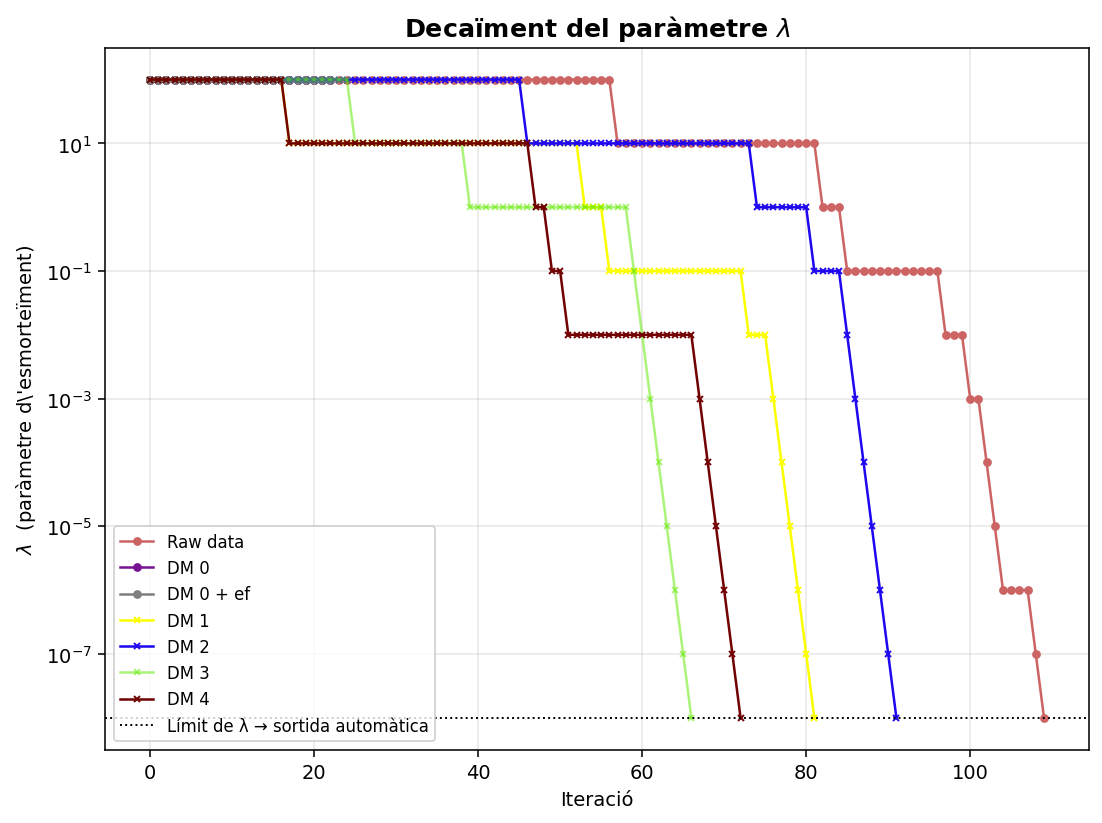
\includegraphics[width=\linewidth]{lambda_decay_base.png}%
    \end{minipage}%
    \hfill
    \begin{minipage}[t]{0.49\textwidth}%
        \centering
        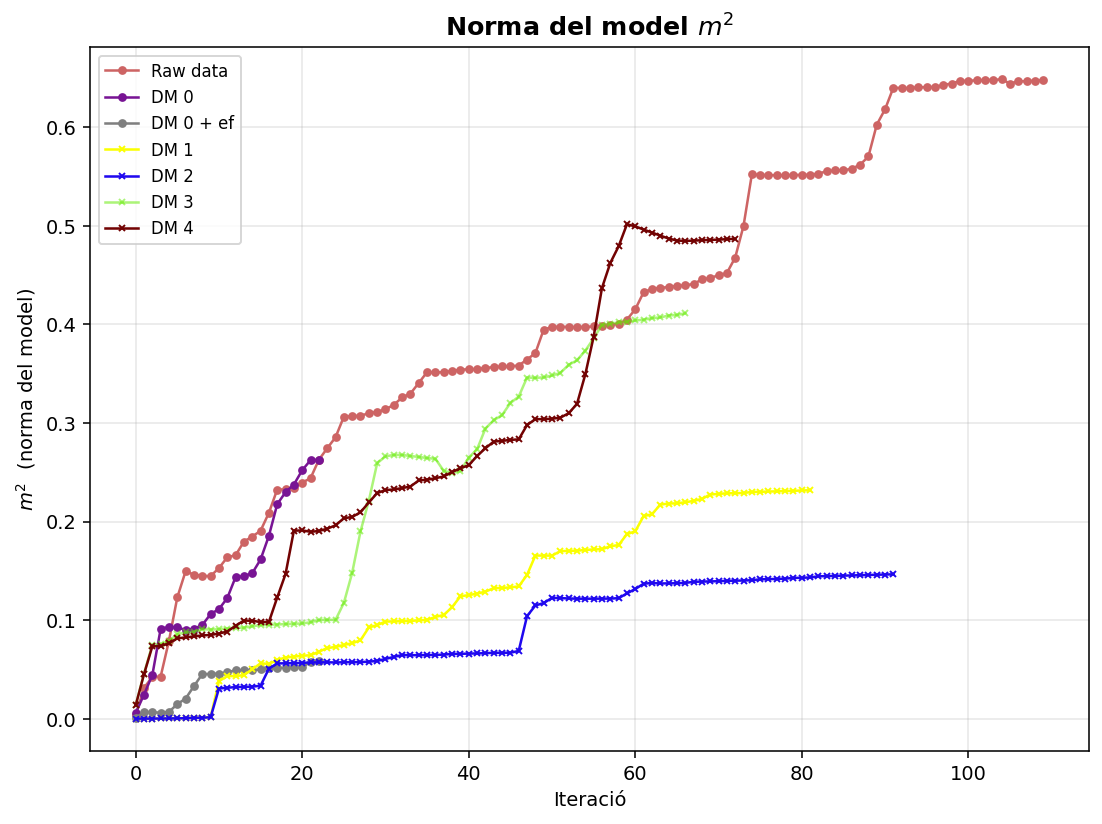
\includegraphics[width=\linewidth]{model_norm_base.png}%
    \end{minipage}
    \caption{Decaïment del paràmetre de regularització $\lambda$ i norma del model $m^2$ en funció de les iteracions executada per ModEM. El gràfic de l'esquerra mostra com s'estableix un límit de decaïment de $10^{-8}$ per $\lambda$. A la dreta s'observa la norma del model que representa la variació o complexitat del model respecte del model inicial $m_0$.}
    \label{fig:lambda-norma}
\end{figure}


\subsection{Elecció del model}


Un cop avaluat el conjunt d'inversions, s'ha adoptat com a model final la
\emph{Depuració Manual~4}. Aquest
model aconsegueix generar prou estructura per resoldre els trets geoelèctrics
d'interès i, alhora, reprodueix un resultat fortament comparable amb l'estudi de
referència \citet{arango2005} (\cref{fig:comparacio-arango}) mentre que aconsegueix disminuir el desajust de les dades taula~\ref{tab:modem_manual} sense recórrer a l'eliminació ni a la devaluació de la informació
tridimensional continguda a les components diagonals.

\vspace{1pt}

\begin{table}[H]
  \centering
  \scriptsize
  \captionsetup{font=scriptsize,skip=3pt}
  \setlength{\tabcolsep}{2.5pt}
  \renewcommand{\arraystretch}{0.92}
  \begin{tabularx}{\textwidth}{@{}lrrrr>{\raggedright\arraybackslash}X@{}}
    \toprule
    \textbf{Assaig} & \textbf{Iter.} & \textbf{RMS ini.} & \textbf{RMS fin.} &
    \textbf{$m^2_{\mathrm{fin}}$} & \textbf{Components} \\
    \midrule
    Raw data & 110 & 48.29 & 14.39 & 0.647
      & Sense depurar; sense floor \\
    \midrule
    DM 0 & 23 & 37.55 & 13.63 & 0.262
      & Depuració manual a $(Z_{xy},Z_{yx})$,  sense floor \\
    \midrule
    DM 0 + ef & 23 & 12.15 & 7.21 & 0.059
      & Depuració manual a $(Z_{xy},Z_{yx})$; floor 5\% de $\sqrt{|Z_{xy}Z_{yx}|}$ a totes les components \\
    \midrule
    DM 1 & 82 & 12.65 & 6.71 & 0.232
      & Floor 5\% de $\sqrt{|Z_{xy}Z_{yx}|}$ a totes les components ($T\le10$\,s) \\
    \midrule
    DM 2 & 92 & 11.10 & 3.81 & 0.146
      & Diagonals depurades manualment; floor 5\% de $\sqrt{|Z_{xy}Z_{yx}|}$ (7\% a les diagonals $(Z_{xx},Z_{yy})$); $T\le10$\,s \\
    \midrule
    DM 3 & 67 & 9.70 & 6.68 & 0.411
      & Floor 5\% de $\sqrt{|Z_{xy}Z_{yx}|}$; $T\le1$\,s \\
    \midrule
    DM 4 & 73 & 8.38 & 4.67 & 0.487
      & Floor 5\% de $\sqrt{|Z_{xy}Z_{yx}|}$ a totes les components; diagonals de mall26/52/53 depurades; $T\le1$\,s \\
    \bottomrule
  \end{tabularx}
  \caption{Inversions ModEM NLCG sobre dades netejades manualment (i cas cru de
    referència): iteracions, RMS inicial i final, norma del model final $m^2$ i
    tractament de les components de la impedància. El floor s'aplica com
    $\sigma=\max(\sigma_{\mathrm{natiu}},\,\mathrm{floor})$.}
  \label{tab:modem_manual}
\end{table}

\vspace{5pt}
\subsubsection{Avaluació de les condicions de contorn}
 
Sobre aquesta base, s'ha decidit acotar el rang de períodes fins a $T = 1$~s. La
justificació és directa a partir de la profunditat de penetració (\emph{skin depth}) taula~\ref{tab:skindepth}. Una estimació més conservadora ve donada per la profunditat de
Niblett--Bostick \citep{niblett1960, bostick1977}, $z_{NB} \approx \delta/\sqrt{2} \approx 356\,\sqrt{\rho\,T}$ . La
taula~\ref{tab:skindepth} recull tots dos valors a $T = 1$~s per a un ventall de
resistivitats representatiu del recobriment de la zona d'estudi.

\vspace{5pt}

 
\begin{table}[H]
    \centering
    
    \begin{tabular}{l r r}
        \toprule
        $\rho$ ($\Omega\cdot m$) & $\delta$ a 1\,s (m) & $z_{NB}$ a 1\,s (m) \\
        \midrule
        5 \ (intrusió salina / conductor) & 1\,125 & 796 \\
        10                                & 1\,591 & 1\,125 \\
        30 \ (mescla sediment/calcària)   & 2\,755 & 1\,949 \\
        100 \ (calcària resistiva)        & 5\,030 & 3\,557 \\
        \bottomrule
    \end{tabular}
    \caption{Profunditat $\delta$ i profunditat de sondeig de
    Niblett--Bostick $z_{NB}$ a $T = 1$~s, segons l'equació~\eqref{eq:15},
    per a diferents resistivitats del recobriment.}
    \label{tab:skindepth}
\end{table}
 
Com es desprèn de la Taula~\ref{tab:skindepth}, fins i tot en el cas més desfavorable per a la penetració —un recobriment fortament conductor de $\rho \approx 5\text{--}10~\Omega\cdot\text{m}$ a $T = 1~\text{s}$—, la profunditat de penetració (\textit{skin depth}) és d'uns $1{,}1\text{--}1{,}6~\text{km}$ i el sondeig efectiu de Niblett--Bostick se situa entre $\sim 0{,}8\text{--}1{,}1~\text{km}$. Totes dues magnituds es troben clarament per sobre de l'objectiu de caracterització, situat a $600\text{--}700~\text{m}$. Invertint l'equació~\eqref{eq:15}, s'observa que per assolir els $700~\text{m}$ només calen períodes de l'ordre de $T = \rho^{-1} (z/503)^{2} \approx 0{,}2~\text{s}$ (per a $\rho = 10~\Omega\cdot\text{m}$) o $0{,}07~\text{s}$ (per a $\rho = 30~\Omega\cdot\text{m}$). D'aquesta manera, l'estructura objectiu queda plenament continguda dins la banda mostrejada i no pas al límit de penetració, on quedaria mal restringida.

\vspace{5pt}

 
Aquesta acotació té, a més, una conseqüència directa sobre el disseny del model. La
condició de contorn inferior del domini tridimensional exigeix que la malla
s'estengui fins a profunditats on els camps electromagnètics siguin negligibles
i s'assoleixi el règim asimptòtic \citep{chavejones2012,egbert2014}.

\vspace{5pt}
Atès que $\delta \propto \sqrt{T}$, reduir el període màxim d'unes desenes
de segons fins a $1$~s disminueix el \emph{skin depth} màxim en el factor
corresponent (per exemple, $\sqrt{10} \approx 3{,}16$ en passar de $10$~s a $1$~s) i,
per tant, la fondària mínima que ha de tenir el model per satisfer la condició de
contorn es redueix en la mateixa proporció. Això permet aprimar el model inicial (taula~\ref{tab:1}), fent-lo compatible amb les condicions de contorn descrites per \citet{chavejones2012}
i alhora, reduir de manera notable el cost computacional de la inversió, sense
comprometre en cap moment la resolució de l'objectiu situat a $600\text{–}700$~m.

\vspace{5pt}
 
Convé matisar que $\delta$  és una aproximació
unidimensional i que en un medi tridimensional la sensibilitat real depèn també de la
cobertura de períodes i de la qualitat de les dades. Tanmateix, el
criteri és plenament vàlid i robust, atès que el marge de penetració respecte a
l'objectiu és ampli fins i tot en el cas més conductor, tal i com es pot veure en la comparació dels models que es realitzarà més endavant.

\subsubsection{Estudi individual de les estacions}

El model escollit (DM 4) ha passat per un procés analític previ, que esdevé del model DM 3, i cal ser avaluat en aquesta secció. A l'apartat 3.2.1 es raona l'elecció del rang de períodes utilitzat per establir un model de referència, mentre que aquí ens enfoquem en l'última passa desenvolupada en aquest treball. Aquest anàlisi final ens ha permès millorar la correlació de les dades significativament, a la vegada que aporta rellevància al mètode algorítmic respecte del mètode d'assaig i error implantat a l'estudi de referència. 

\vspace{5pt}

Per avaluar el grau d'ajust del model final i entendre com cal interpretar el desajust, la taula~\ref{tab:rms-estacions-ext} recull les tres estacions amb els valors de RMS més baixos i més alts, mentre que la taula~\ref{tab:rms-periodes-ext} presenta la mateixa selecció en funció del període. En ambdues taules, les dades es desglossen en la contribució total, la de les components antidiagonals (\textit{ad}) i la de les diagonals (\textit{diag}), juntament amb l'error relatiu mitjà $\overline{e/|Z|}$\footnote{A l'equació~\eqref{eq:17}, $\sigma_i$ és l'error assignat a cada dada
individual. Si definim $|Z_{c,T}|=\sqrt{\operatorname{Re}(Z_{c,T})^2+\operatorname{Im}(Z_{c,T})^2}$
on $c$ és la component diag/ad i $T$ el període, l'error relatiu tabulat és la mitjana d'aquests
quocients sobre el grup, $\overline{e/|Z|}=\big\langle \sigma_{c,T}/|Z_{c,T}|
\big\rangle$, amb $e\equiv\sigma$.}

\vspace{5pt}

El punt clau d'aquests resultats està en que els elevats valors de l'RMS total, venen derivats pràcticament en la seva totalitat, de les components diagonals, ja que aquestes no han sigut depurades per preservar la informació tridimensional que presenta el sistema estudiat. D'acord amb la taula~\ref{tab:rms-estacions-ext}, les estacions amb pitjor ajust són la 26, 52 i 53 (\cref{fig:rms-estacions-mapa}). La taula~\ref{tab:rms-periodes-ext} mostra el mateix patró per als períodes amb més desajust, especialment al voltant de $1{,}00\times10^{-2}$ o 50  $Hz$, que és el mateix (\cref{fig:interferencia-50hz}). En totes dues taules, l'antidiagonal presenta un $\overline{e/|Z|}$ baix i estable ($0{,}05$--$0{,}09$), mentre que la diagonal mostra valors més elevats ($0{,}15$--$0{,}48$), característics de components petites i sorolloses que queden menys restringides durant la inversió.

\vspace{5pt}
La lectura conjunta de les taules~\ref{tab:rms-estacions-ext} i~\ref{tab:rms-periodes-ext} reforça la idea de que un RMS més baix no implica necessàriament que la resposta del model s'aproximi millor a les dades observades. Com que l'RMS és un desajust normalitzat per l'error, $r = (d^{\text{obs}} - d^{\text{pred}})/\sigma$, la seva interpretació depèn tant del residu com de la incertesa assignada a cada component. Per això, els valors de les columnes \textit{total}, \textit{ad} i \textit{diag} s'han d'analitzar juntament amb les columnes de $\overline{e/|Z|}$.
\vspace{5pt}


\noindent
\begin{minipage}[t]{0.49\textwidth}
  \vspace{0pt}
  \centering
  \footnotesize
  \setlength{\tabcolsep}{3pt}
  \captionsetup{hypcap=false}
  \begin{tabular}{@{}lccccc@{}}
    \toprule
    Estació & \multicolumn{3}{c}{RMS} & \multicolumn{2}{c}{$\overline{e/|Z|}$} \\
    \cmidrule(lr){2-4}\cmidrule(lr){5-6}
     & total & ad & diag & ad & diag \\
    \midrule
    \multicolumn{6}{l}{\textit{3 més baixos}} \\
    mall31 & 1.08 & 1.13 & 1.02 & 0.05 & 0.26 \\
    mall65 & 1.37 & 1.61 & 1.18 & 0.05 & 0.48 \\
    mall14 & 1.56 & 1.67 & 1.45 & 0.05 & 0.34 \\
    \midrule
    \multicolumn{6}{l}{\textit{3 més alts}} \\
    mall26 & 23.02 & 4.19 & 28.71 & 0.06 & 0.35 \\
    mall52 & 17.44 & 3.88 & 23.57 & 0.06 & 0.21 \\
    mall53 & 11.84 & 2.22 & 15.21 & 0.06 & 0.25 \\
    \bottomrule
  \end{tabular}
  \captionof{table}{RMS normalitzat i error relatiu mitjà per estació del model DM 3.}
  \label{tab:rms-estacions-ext}
\end{minipage}\hfill
\begin{minipage}[t]{0.49\textwidth}
  \vspace{0pt}
  \centering
  \footnotesize
  \setlength{\tabcolsep}{3pt}
  \captionsetup{hypcap=false}
  \begin{tabular}{@{}lccccc@{}}
    \toprule
    Període (s) & \multicolumn{3}{c}{RMS} & \multicolumn{2}{c}{$\overline{e/|Z|}$} \\
    \cmidrule(lr){2-4}\cmidrule(lr){5-6}
     & total & ad & diag & ad & diag \\
    \midrule
    \multicolumn{6}{l}{\textit{3 més baixos}} \\
    $2.56\times10^{-1}$ & 1.99 & 1.95 & 2.03 & 0.07 & 0.36 \\
    $3.44\times10^{-1}$ & 2.10 & 1.96 & 2.21 & 0.09 & 0.40 \\
    $7.59\times10^{-3}$ & 2.21 & 1.71 & 2.62 & 0.05 & 0.34 \\
    \midrule
    \multicolumn{6}{l}{\textit{3 més alts}} \\
    $1.83\times10^{-2}$ & 23.32 & 4.19 & 28.76 & 0.05 & 0.15 \\
    $1.31\times10^{-3}$ & 13.31 & 4.86 & 15.57 & 0.05 & 0.18 \\
    $1.02\times10^{-2}$ & 11.37 & 3.38 & 14.56 & 0.05 & 0.26 \\
    \bottomrule
  \end{tabular}
  \captionof{table}{RMS normalitzat i error relatiu mitjà per període del model DM 3.}
  \label{tab:rms-periodes-ext}
\end{minipage}

\vspace{5pt}



\vspace{5pt}

\noindent
\begin{minipage}[t]{0.49\textwidth}
    \vspace{0pt}
    \centering
    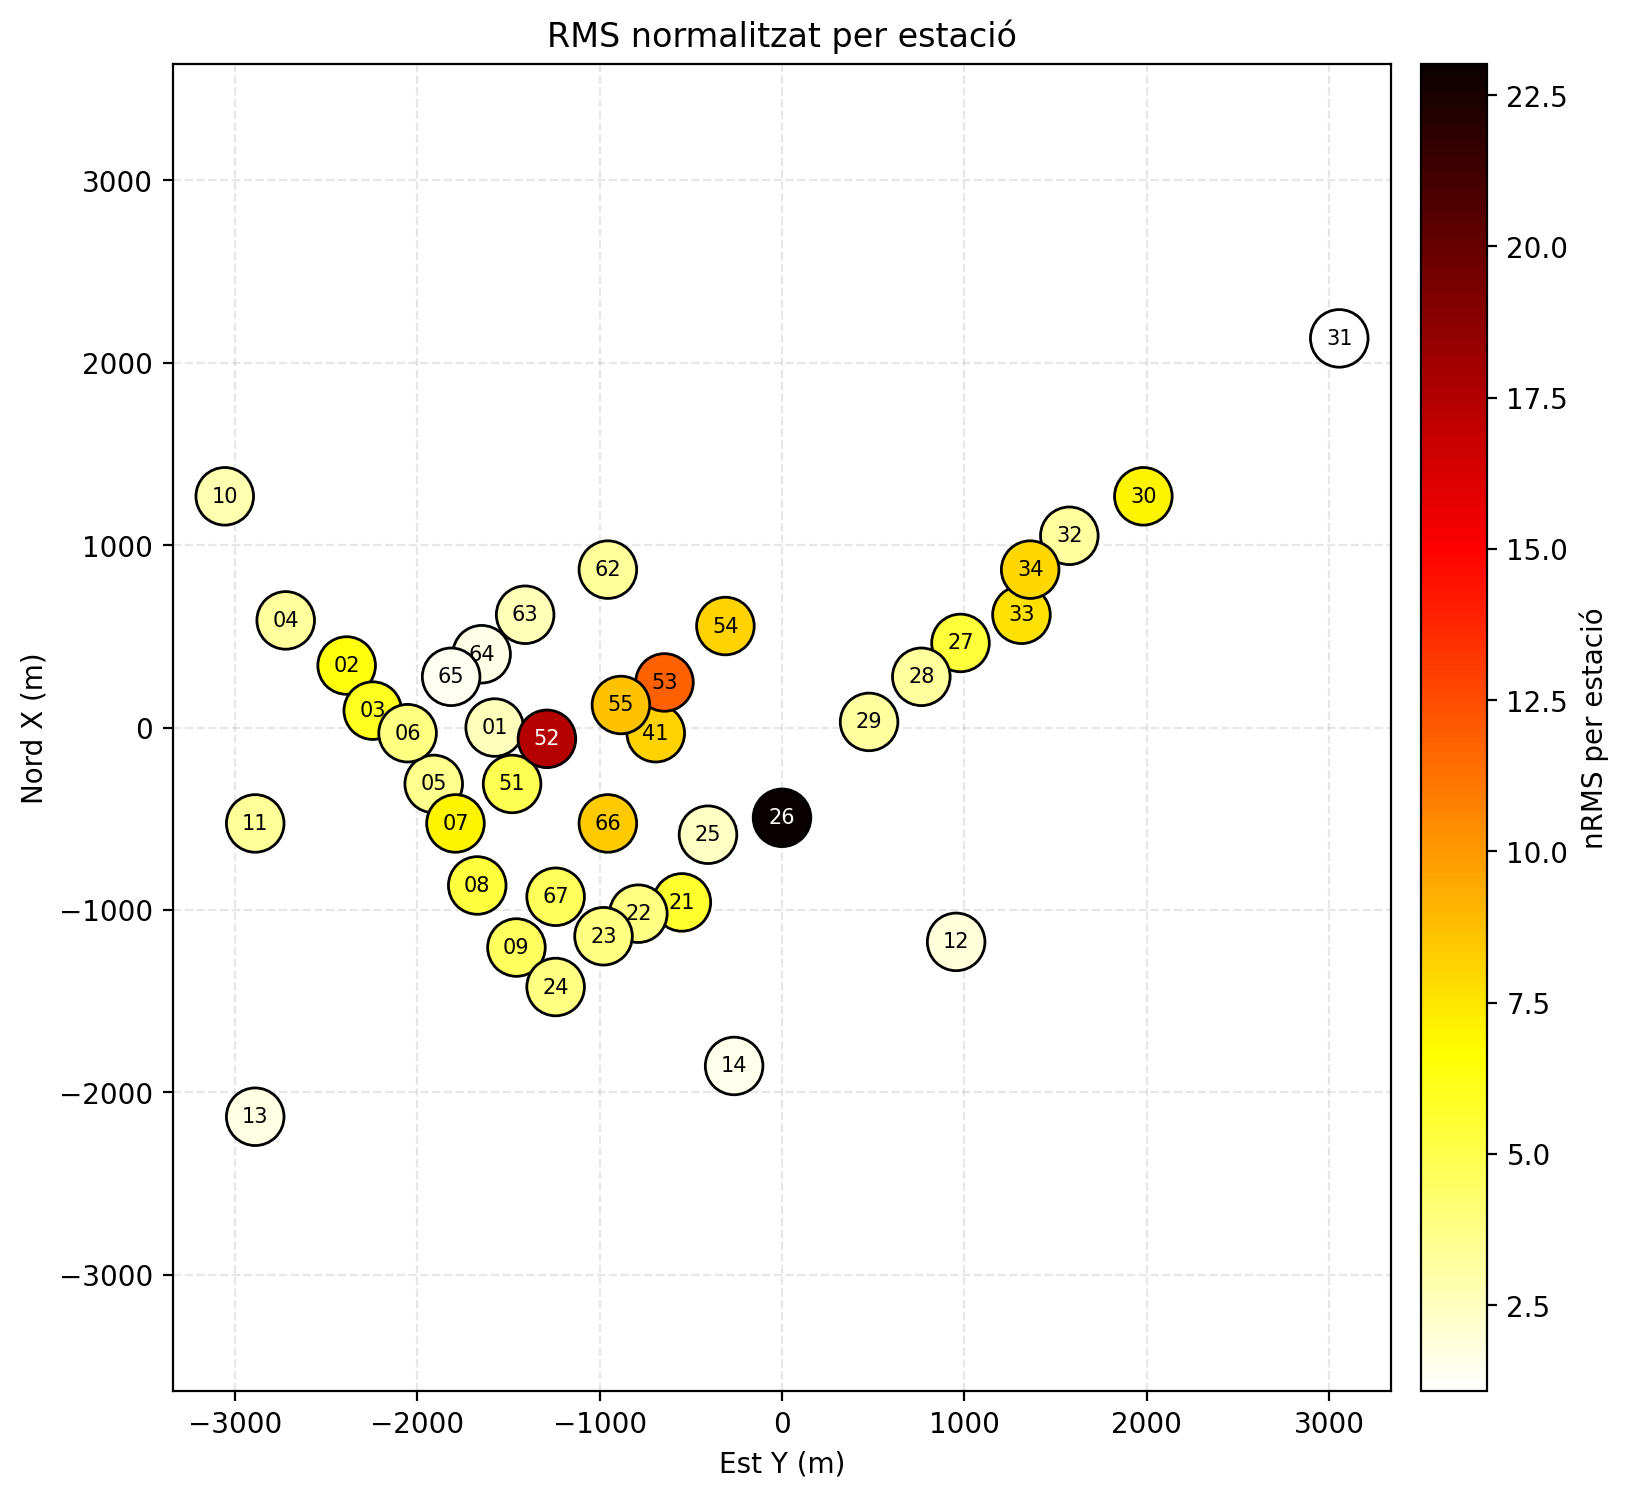
\includegraphics[width=\linewidth,height=0.23\textheight,keepaspectratio]{rms_station_map.png}
    \captionsetup{hypcap=false}
    \captionof{figure}{Distribució espacial de l'RMS per estació del model DM 3.}
    \label{fig:rms-estacions-mapa}
\end{minipage}\hfill
\begin{minipage}[t]{0.49\textwidth}
    \vspace{0pt}
    \centering
    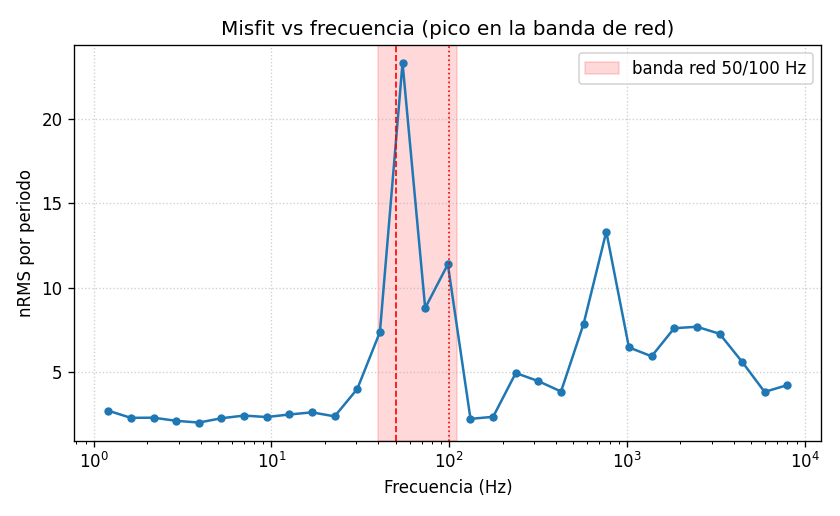
\includegraphics[width=\linewidth,height=0.23\textheight,keepaspectratio]{powerline_nRMS_vs_freq.png}
    \captionsetup{hypcap=false}
    \captionof{figure}{RMS en funció de la freqüència del model DM 3.}
    \label{fig:interferencia-50hz}
\end{minipage}

\vspace{5pt}

La (\cref{fig:interferencia-50hz}) mostra un comportament anòmal que ja hem introduït amb anterioritat però que cal matisar. Clarament la freqüència dels 50 $Hz$ presenta un pic que es pot interpretar com una font de soroll originària de les mesures, en concret per l'estació 26. Encara que les dades proporcionades ja han passat per un processament previ, aquest pic no representa la realitat geològica del subsòl. La morfologia de les dades ens indica que és soroll cultural (\textit{powerline noise}) possiblement causat per la proximitat d'un post de la xarxa elèctrica (s'ha pogut corroborar a partir de l'ubicació de l'estació 26). Com que la xarxa elèctrica nacional opera precisament a $50~\text{Hz}$, la contaminació queda concentrada en aquesta freqüència i no s'estén de manera suau per la resta de la corba (\cref{fig:comparacio-depuracio-26},\cref{fig:ajusts}). A més, si el corrent de la línia elèctrica arriba a pertorbar la mesura, els camps elèctric i magnètic entren en fase (\cref{fig:comparacio-depuracio-26}) \citep{szarka1988}, tal i com podem observar a la Figura \ref{fig:comparacio-depuracio-26}.
\vspace{5pt}

També localitzem un altre pic a al rang dels 1-5 kHz, el qual coincideix amb la banda morta característica de l'AMT i de fenomenologia atmosfèrica \citet{garcia2002}
\vspace{5pt}

Aquest fonament va conduir a la depuració manual (DM 4) de les diagonals, per les dades que envolten aquesta freqüència en les estacions 26, 53 i 52, proporcionant un RMS de 4.67 que disminueix 2 punts el desajust i incrementa un 18\% la norma $m^2$ respecte del model DM 3 (taula~\ref{tab:modem_manual}), alhora millorant el resultat de RMS = 6.07 obtingut per \citet{arango2005} sense perdre informació geofísica essencial.


\subsection{Ajust de les dades}

Ara que ja hem escollit el model que volem representar, resulta interessant visualitzar com s'ha formalitzat l'ajust. Per això a la (\cref{fig:ajusts}) es mostren les corbes $\log_{10}(\rho_a)$ vs $\log_{10}(T)$ predites en 4 estacions diferents.

\vspace{5pt}

Per tenir una visió concreta a partir d'una petita mostra de les estacions disponibles, s'ha optat per escollir el mateix subconjunt que a l'apartat 2.2.3, amb una diferència essencial, aquí es mostren les components de la diagonal $Z_{xx}, Z_{yy}$, que apareixen sense depurar ( a excepció de l'estació 26).

\vspace{5pt}


\begin{figure}[H]
  \centering
  
  % --- IMATGE DE DALT ---
  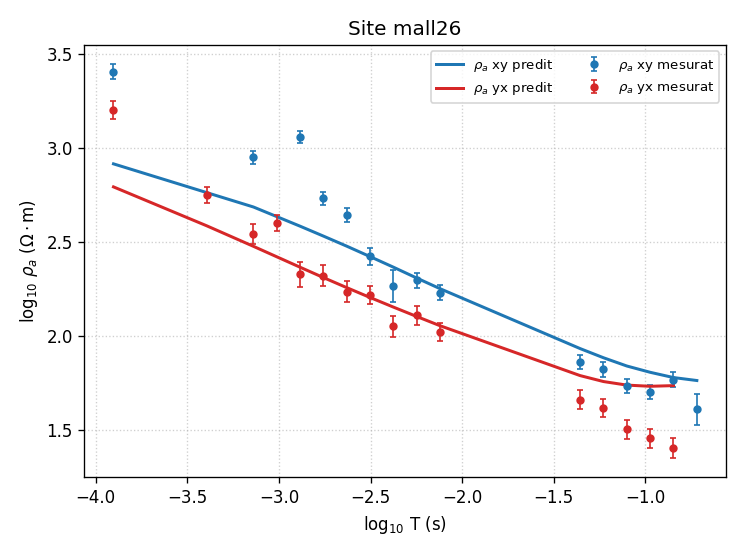
\includegraphics[width=0.75\textwidth]{mall26.png}
  
  \vspace{0.3cm} % Espai vertical intermedi

  % --- IMATGES DE BAIX ---
  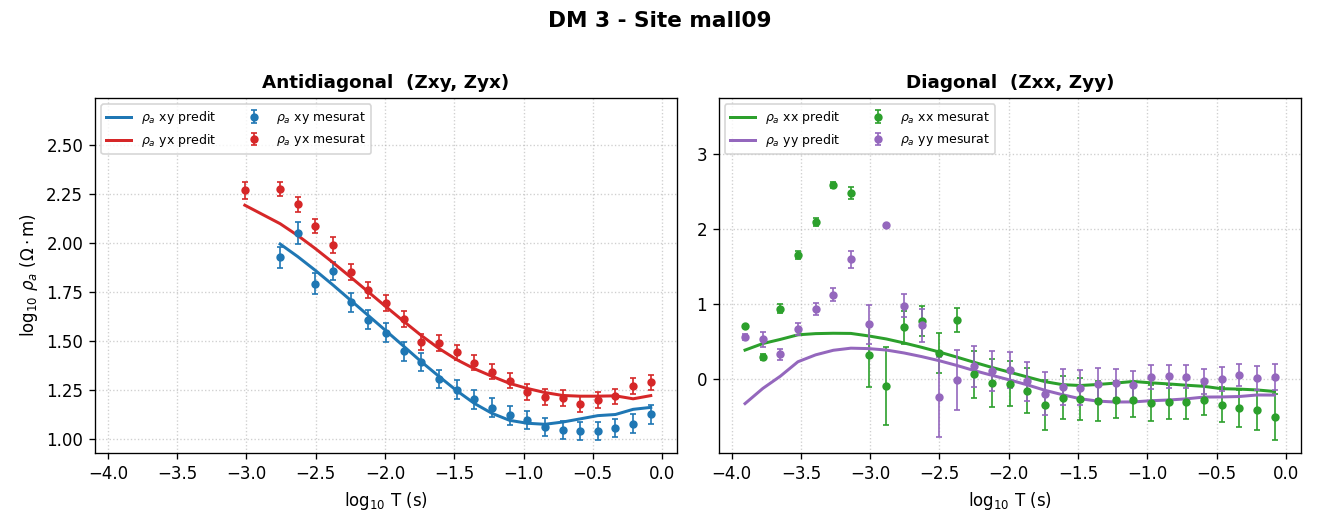
\includegraphics[width=0.49\textwidth]{mall09.png}
  \hfill % Espai horitzontal per separar-les
  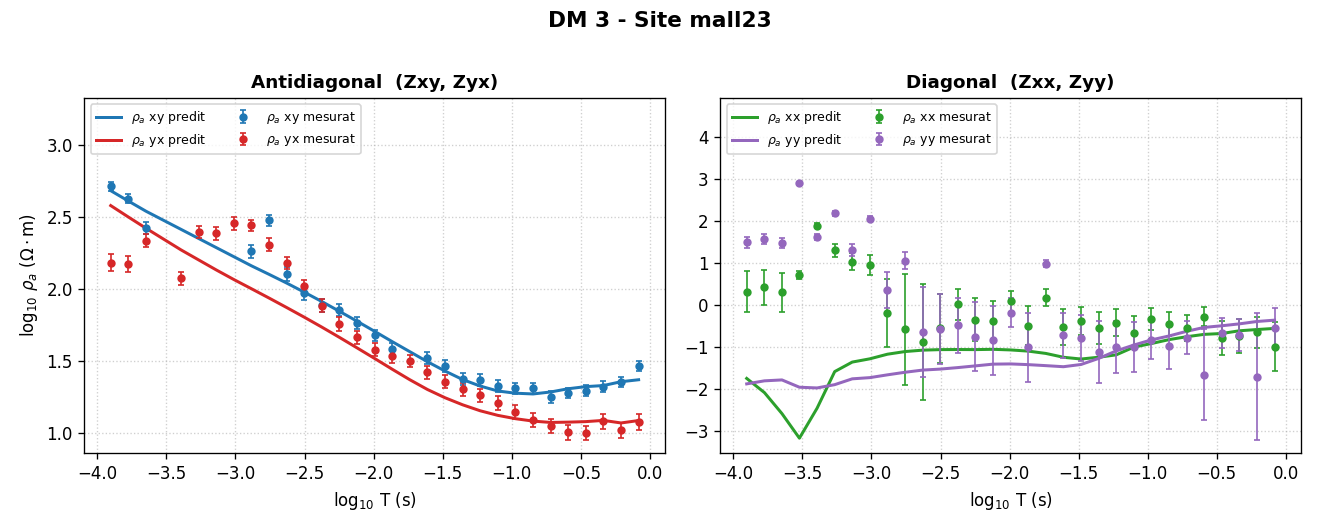
\includegraphics[width=0.49\textwidth]{mall23.png}

  \caption{Títol de la figura amb les tres imatges.}
  \label{fig:ajusts}
\end{figure}



\vspace{5pt}

Podem comentar l'efectivitat de l'algorisme per evadir pertorbacions característiques del renou experimental i la capacitat d'ajustar i suavitzar les prediccions sobretot per les components depurades.

\subsection{Interpretació del model}

Finalment procedim a visualitzar els resultats que ens aporten la part més il·lustradora de l'investigació. A continuació seccionarem l'estructura geoelèctrica per ajudar-nos a inferir els tipus de materials que resideixen en el subsòl del sistema aqüífer de Llucmajor.

\subsubsection{Perfil Vertical}

La zona resistiva superficial s'interpreta com l'aqüífer lliure, el qual presenta un gruix aproximat de $150~\text{m}$ coherent amb la informació procedent dels pous d'explotació \citep{igme2003,arango2005}. Per sota d'aquesta capa, entre els $200$ i els $700~\text{m}$ de profunditat, s'identifica una línia conductora ($\sim 10~\Omega\cdot\text{m}$) associada a un aqüitard, sota la qual es detecta l'aqüífer confinat, caracteritzat per valors de resistivitat entorn dels $100~\Omega\cdot\text{m}$. La localització d'aquests perfils i de les estacions corresponents es detalla a la (\cref{fig:estacions}).

\vspace{5pt}

\begin{figure}[H]
    \centering
    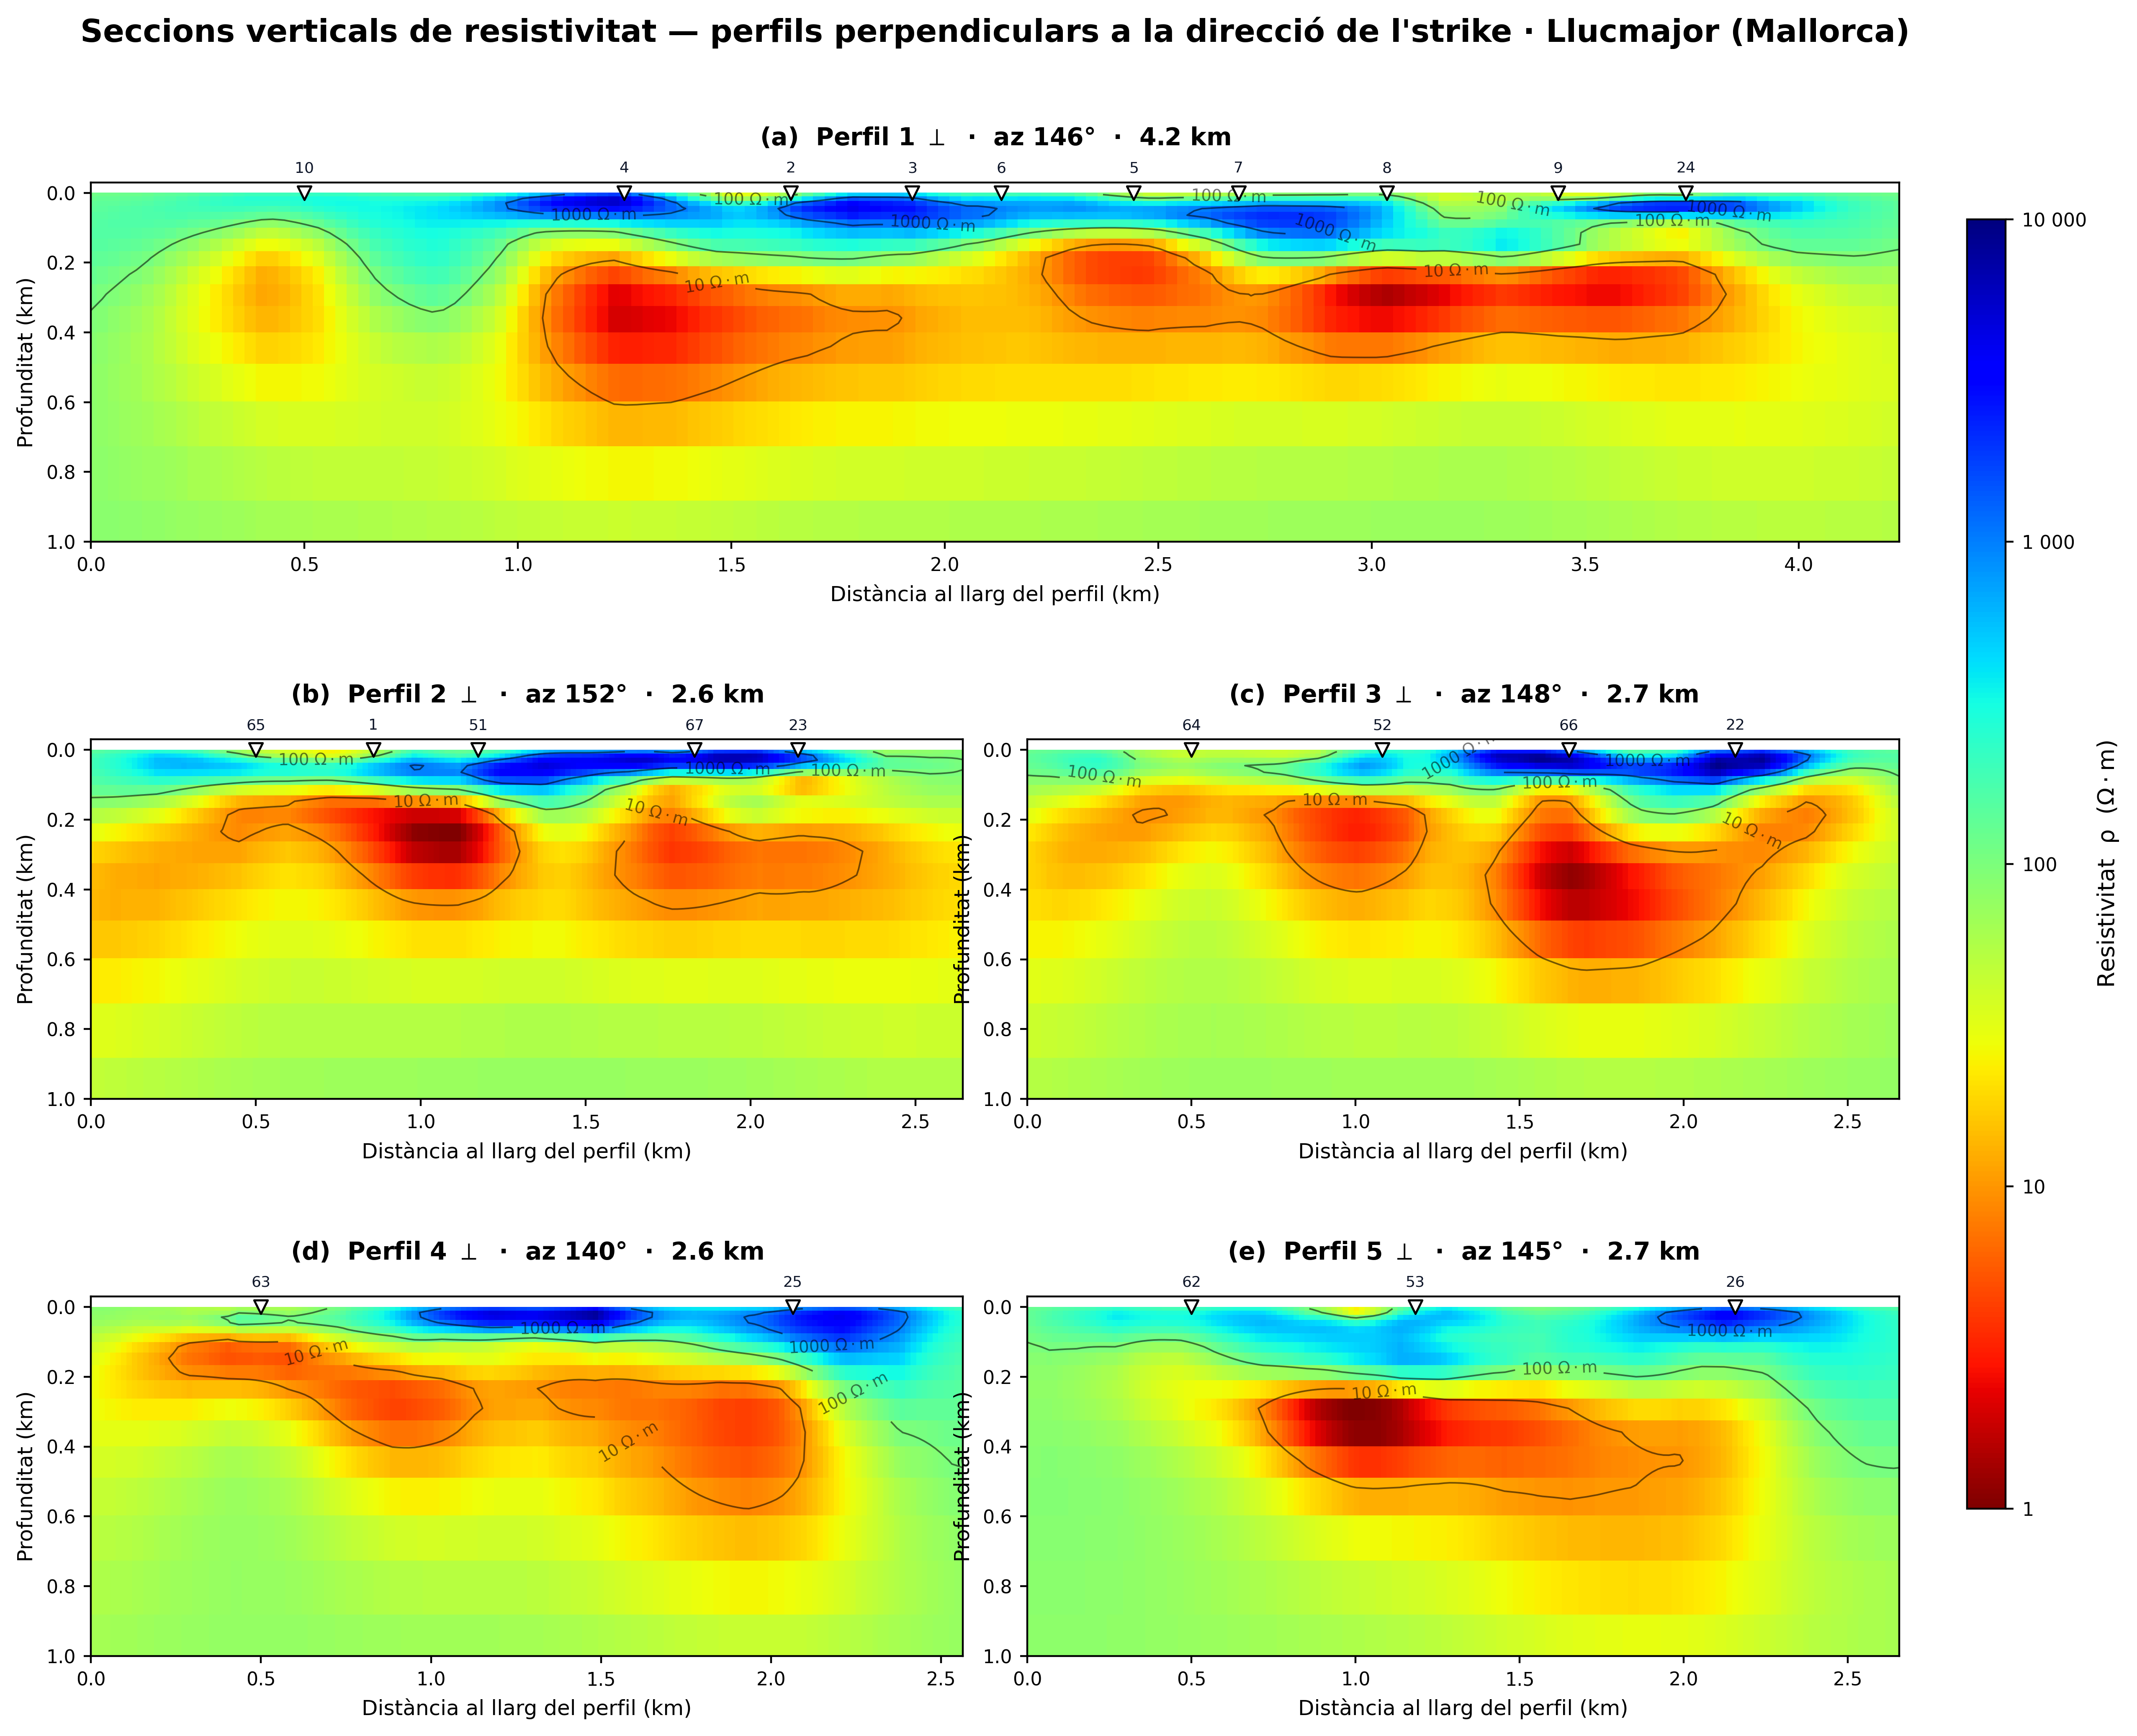
\includegraphics[width=0.65\textwidth]{cross_sections_perpendicular_figure.png}
    \caption{Seccions de resistivitat perpendiculars als perfils d'estacions.}
    \label{fig:perfils-perpendiculars}
\end{figure}


Pel que fa a la resposta hidrogeològica i tèrmica, s'observen discontinuïtats del bloc conductor a la majoria dels perfils. Al perfil 1; entre les estacions 10--4, al perfil 2; entre les estacions 51--67, al perfil 4; per sota de l'estació 26 i al perfil 5 és on hi ha una clara reducció de l'aqüitard. Hem de tenir en compte que l'aigua filtrada no ascendeix de manera totalment vertical degut als materials que impedeixen el seu pas a mesura que va ascendint, per això no hem d'ubicar aquestes anomalies tèrmiques just a sobre de les discontinuïtats sinó allà on hi apareixen zones de color blau cel $\sim 200~\Omega\cdot\text{m}$ ja que es pot relacionar amb la presència d'aigua dolça subterrània. Si ens fixem en el perfil 5 (62--53), podem ubicar aquesta zona allà on les temperatures són de $\approx~50^\circ\text{C}$, al igual que el perfil 3 (1--51) on s'hi mostra una zona amb temperatures de $\approx~40^\circ\text{C}$ {fig:gradient-termic} \citep{igme2003} i coincideix amb la resistivitat mencionada. 

\vspace{5pt}

D'altra banda, al perfil 1 destaca una interrupció de l'aqüitard entre les estacions 10 i 4, acompanyada d'una zona resistiva ben definida al voltant de l'estació 4, la qual es pot relacionar amb la presència d'aigua dolça. De manera anàloga als perfils anteriors, es pot situar aquest resultat en el mapa de temperatures de l'aigua i observar que la zona coincideix de nou amb una anomalia tèrmica al voltant dels $40~^\circ\text{C}$.

\vspace{5pt}
En comparar els perfils generats amb el model de referència \citep{arango2005}, s'observa que les zones resistives i conductores coincideixen amb rangs de resistivitat i similar localització, sumat a que el model actual ofereix una resolució espaial visiblement més elevada.

\vspace{5pt}

Pel que fa al Perfil~1 \cref{compare_profiles_arango_figure.png}, les principals similituds resideixen en l'aprimament de l'aqüitard per sota de l'estació~6 i a partir de l'estació~4. A més, les estructures conductores mostren un acord excel·lent entre ambdós models, especialment en els sectors associats a la presència d'aigua entorn de les estacions 2--3, 4 i 7--8.

\vspace{5pt}

\begin{figure}[H]
  \centering
  \captionsetup{font=small}
  \begin{minipage}[t]{0.49\textwidth}
    \centering
    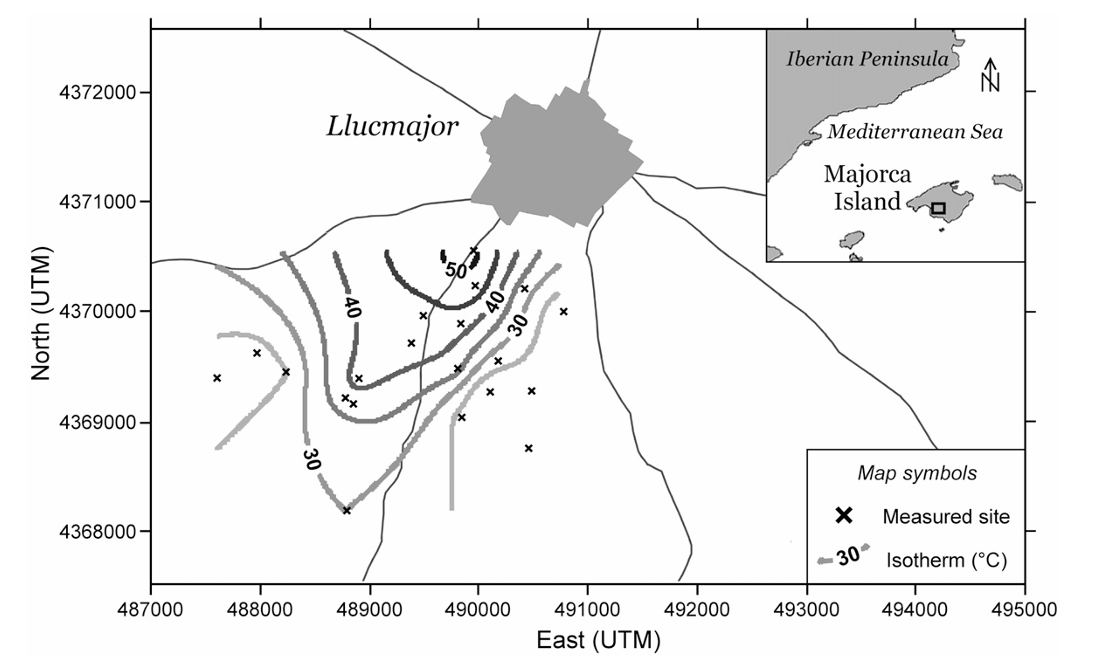
\includegraphics[width=\linewidth]{Gradient_tèrmic.png}
    \captionof{figure}{Gradient tèrmic de la zona de Llucmajor, adaptat de \citet{igme2003}.}
    \label{fig:gradient-termic}
  \end{minipage}\hfill
  \begin{minipage}[t]{0.49\textwidth}
    \centering
    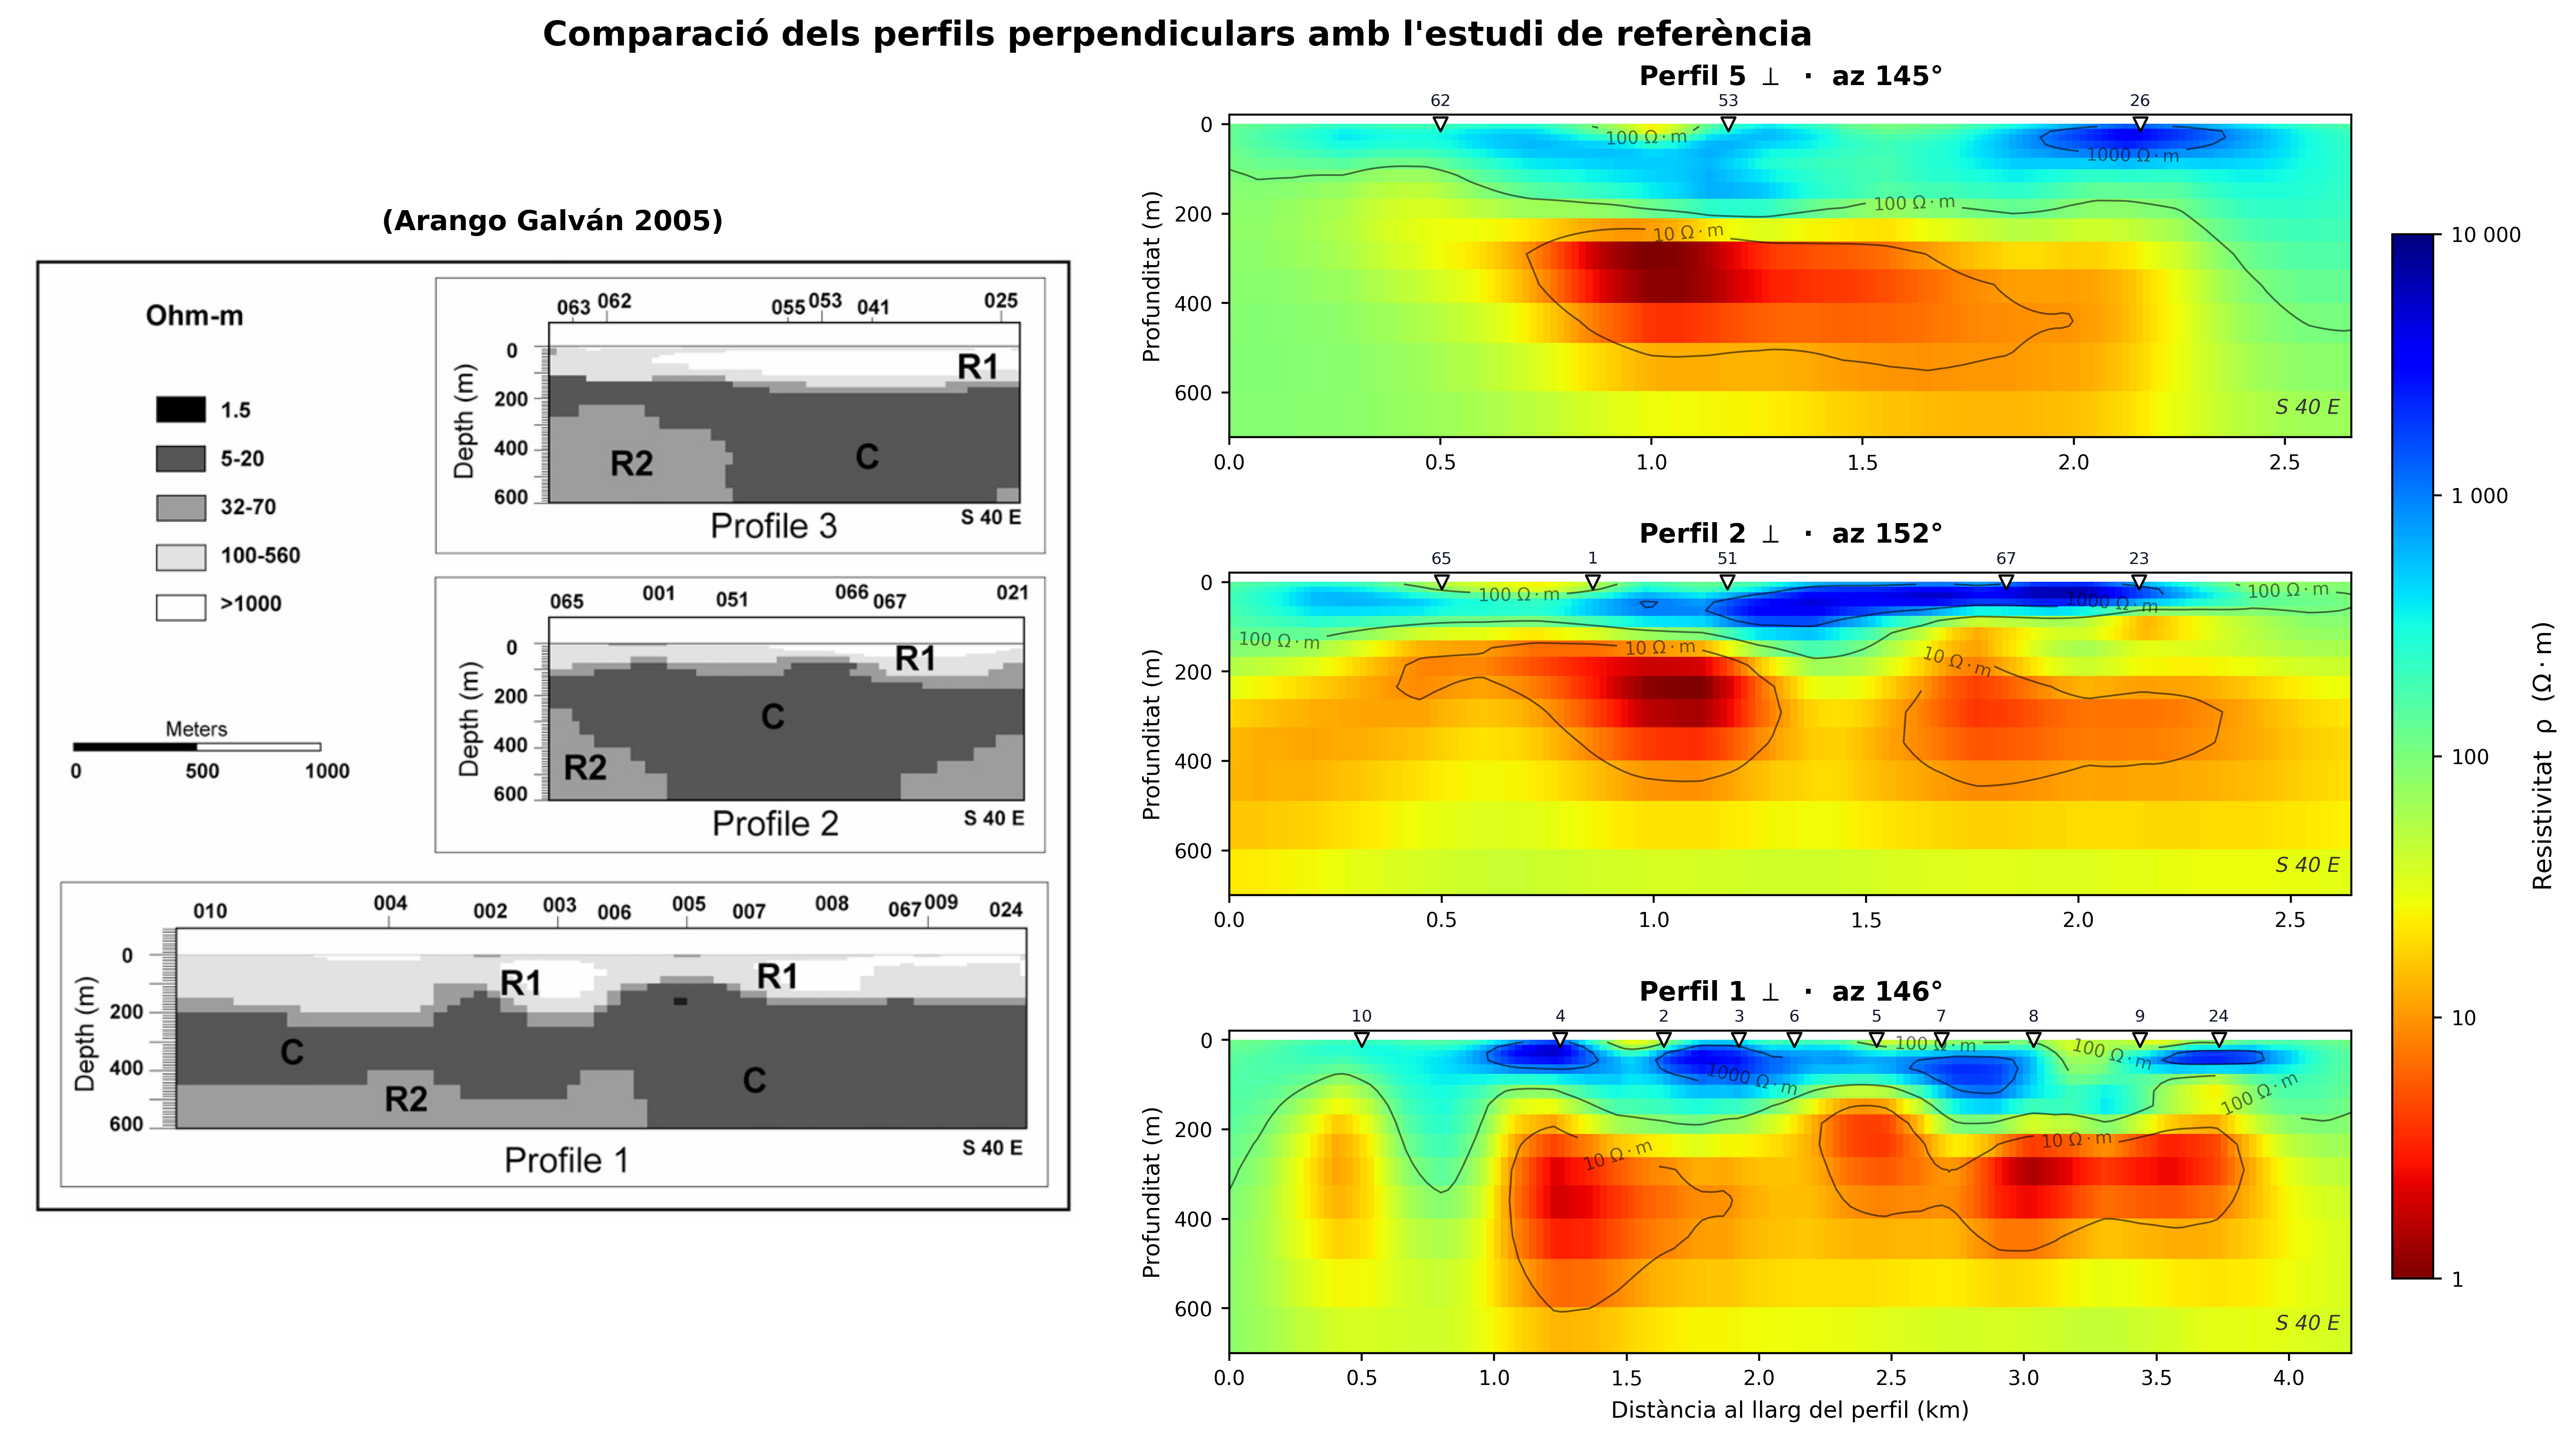
\includegraphics[width=\linewidth]{compare_profiles_arango_figure.png}
    \captionof{figure}{Comparació dels perfils del model final amb els resultats de \citet{arango2005}.}
    \label{fig:comparacio-arango}
  \end{minipage}
\end{figure}



\vspace{5pt}



En el Perfil~2, la morfologia general és molt similar a la descrita anteriorment. Destaca especialment la màxima profunditat de la zona de confinament al voltant de l'estació~51, així com la presència de la franja resistiva superficial a l'entorn de l'estació~67.

\vspace{5pt}

Respecte al Perfil~3, s'identifica el mateix gruix mínim de l'aqüitard a l'altura de l'estació~63. No obstant això, a diferència del model previ, el model d'aquest treball resol una discontinuïtat clarament definida en aquest sector.

\subsubsection{Perfil Horitzontal}

Si canviem la perspectiva i ens fixem en les seccions horitzontals podem veure zones superficials altament resistives $ > 1000\Omega\cdot\text{m}$, que es relacionen amb la presència de roca calcària fossilitzada. A partir dels 200m de fondària, hi trobem la capa de confinament formada per margues, una roca sedimentària composta principalment per argiles i carbonat de calci. La seva resistivitat pot variar entre els  $10 - 200\Omega\cdot\text{m}$ depenent de les condicions d'humitat, la compactació i l'edat geològica de la formació \citep{palacky1987}. Donat que el nostre model recull valors d'uns $1 - 50\Omega\cdot\text{m}$, aquesta teoria reforça la idea de possibles filtracions a través de l'aqüitard.


\begin{figure}[H]
    \centering
    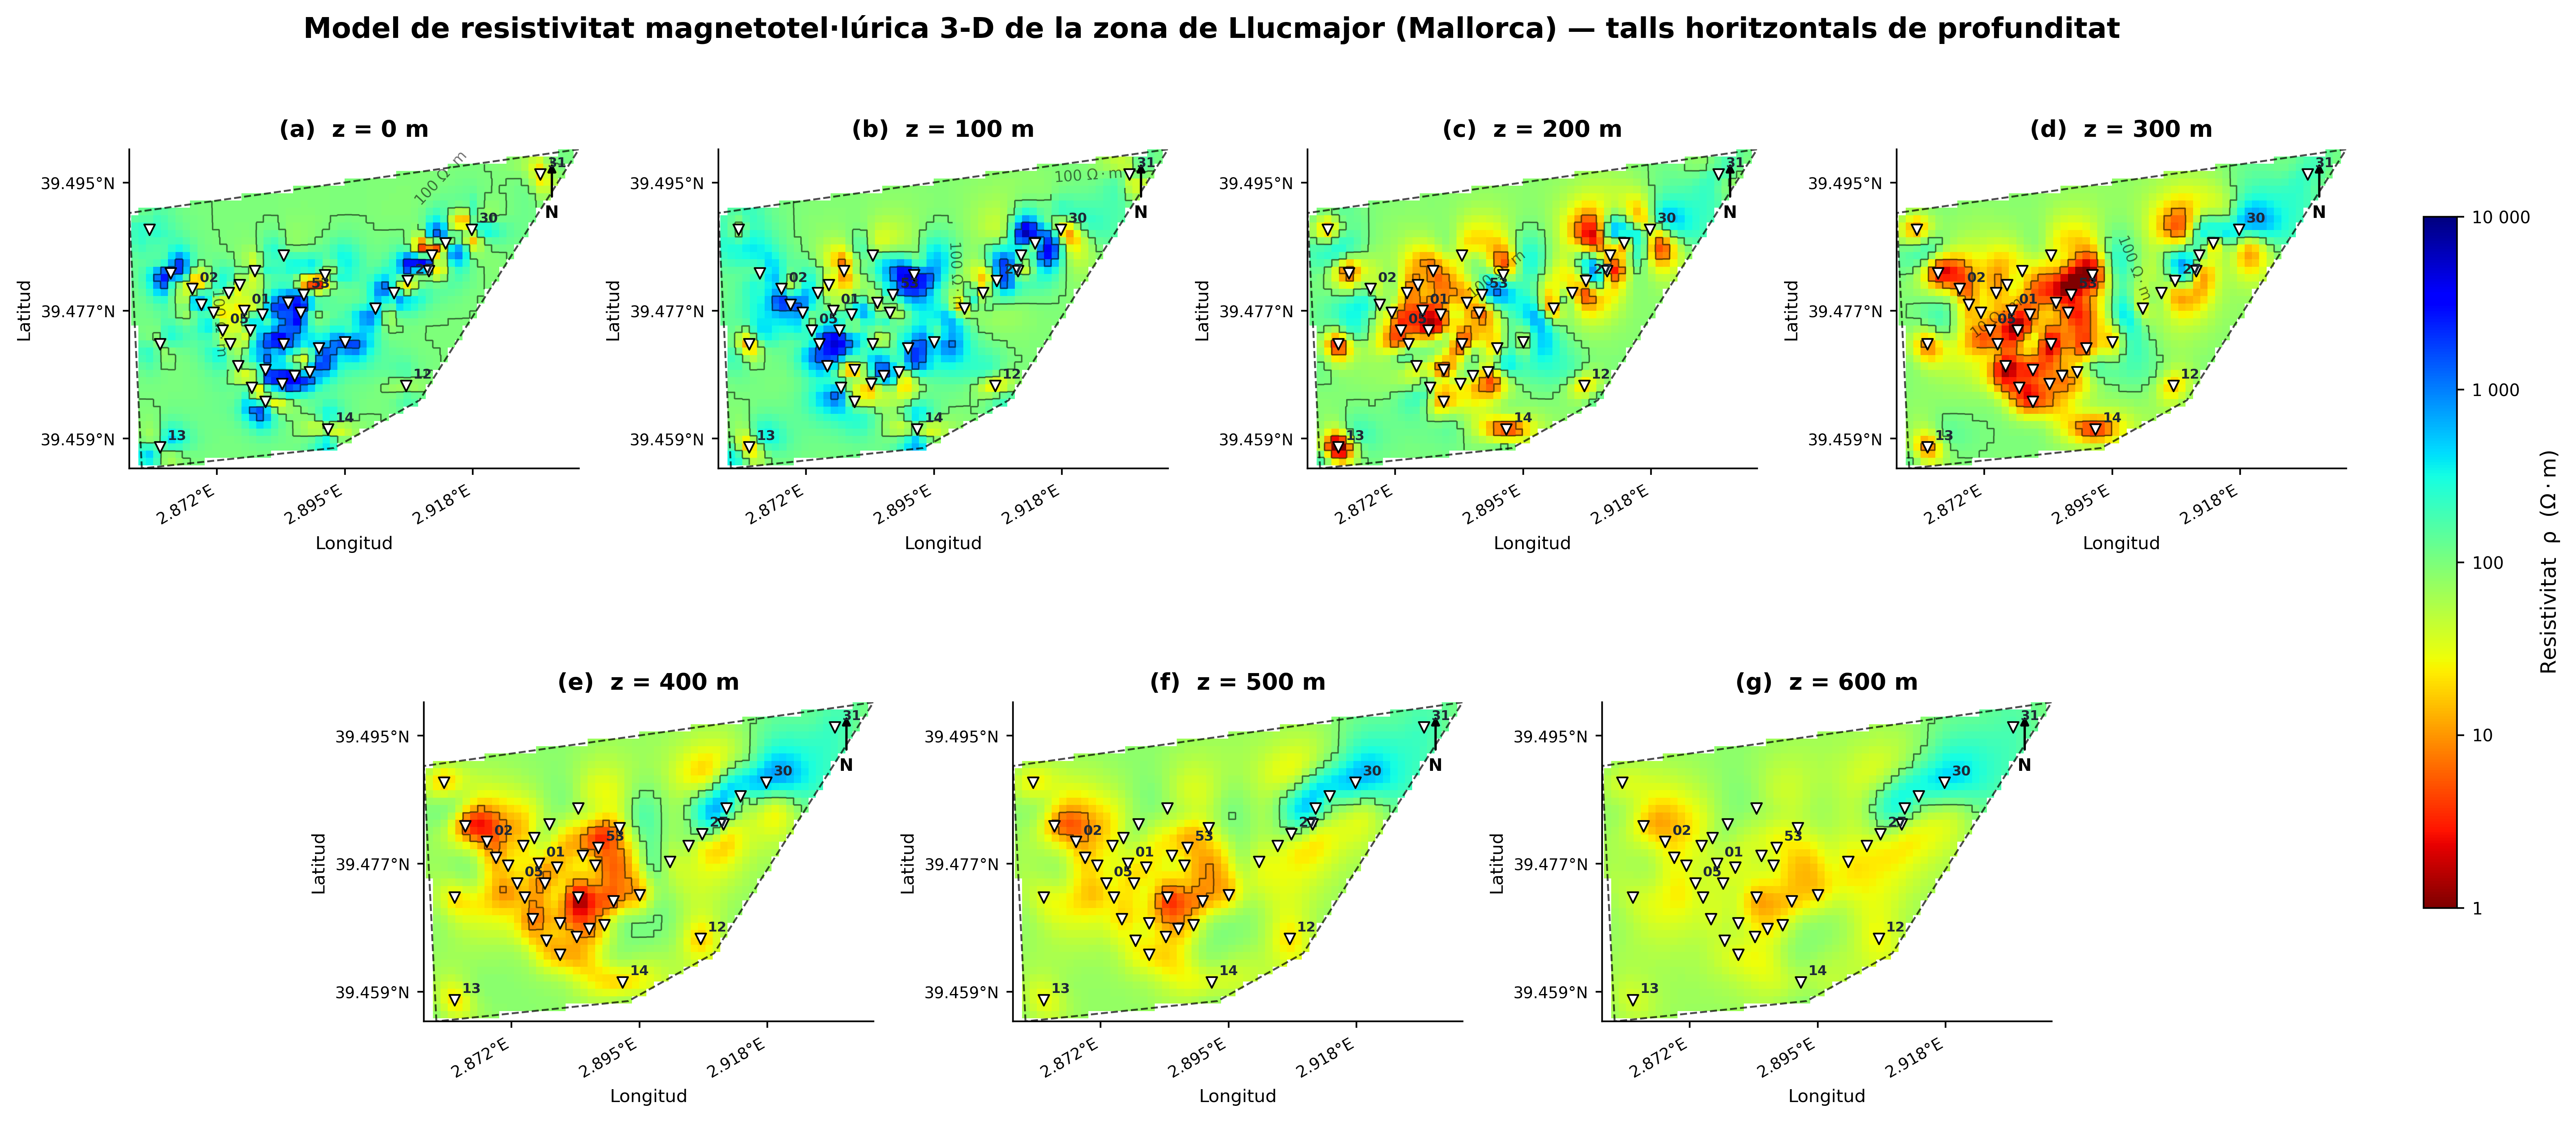
\includegraphics[width=\textwidth,height=0.35\textheight,keepaspectratio]{depth_slices_figure.png}
    \caption{Talls horitzontals del model DM 4 a diferents profunditats.}
    \label{fig:talls-profunditat}
\end{figure}

\vspace{5pt}
Per comparar aquests perfils amb l'estudi de referència, observam la comparació representada a la (\cref{fig:annex-comparacio-talls-arango}), inclosa a l'apèndix~\ref{annex:comparacio-talls-arango}. En aquest cas les similituds no són tan evidents, sobretot per la diferència de resolució existent entre cadascun; no obstant això, la semblança general és perfectament identificable.

\vspace{5pt}

Dels 0 als 200 metres els dos models presenten zones resistives a excepció de la banda N-E de la delimitació mostrada. A partir d'aquell nivell la capa conductora concorda de manera plausible, deixant ara una zona més conductora a la banda N-E.

\vspace{5pt}

La comparació entre les seccions bidimensionals de l'investigació proposada per \citet{arango2005} i la del present treball, enfronta dos mètodes computacionals diferents: l'algorisme d'inversió 2D REBBOC \citep{siripunvaraporn2000} contra l'NLCG \citep{rodi2001}. Com ja hem vist, hi ha similituds evidents entre models però és important tenir en compte que l'anterior utilitza una aproximació d'estructura 2D, inapropiada i insuficient per caracteritzar en detall un sistema geoelèctric amb un grau de tridimensionalitat elevat.  


\section{Discussió i conclusions}

Desenvolupar un model geoelèctric 3D a partir d'un algorisme d'inversió adaptat a la dimensió corresponent, facilita la reproductibilitat i l'objectivitat d'aquesta pràctica, en concret, per a estructures amb manca de simetria bidimensional, com és el cas del sistema aqüífer de Llucmajor.

\vspace{5pt}


Amb l'ajuda essencial de la potència computacional i la seva aplicació a la magnetotel·lúrica, s'ha fet posible l'experimentació amb models tridimensionals complexos que ofereixen resultats diàriament. Atesa la no-unicitat del probema invers, aques ventall de solucions reforça la veracitat de les interpretacions geofísiques.

\vspace{5pt}

El mètode empleat, a part d'aportar rigor científic, incorpora un grau de resolució superior a la representació resistiva de l'indret i manté la morfologia del model proposat per \citet{arango2005}, proporcionant una evidència addicional ben fonamentada que reforça la hipòtesi sobre la discontinuïtat de l'aqüitard existent entre l'aqüífer lliure i el confinat. 



\clearpage


%=====================================================================
%  REFERÈNCIES BIBLIOGRÀFIQUES
%=====================================================================
% La citació al cos és autor-any, però la llista bibliogràfica es numera.
\setcitestyle{numbers,square}
\begin{thebibliography}{99}

\bibitem[Arango Galv\'an(2005)]{arango2005} Arango Galv\'an, C. (2005).
  \textit{Estudi magnetotel\`uric de la zona de Llucmajor (Mallorca): Avances en el proceso de datos y modelo 3D}.
  Tesi doctoral, Universitat de Barcelona.

\bibitem[Benedicto et al.(1993)]{benedicto1993} Benedicto, A., Ramos-Guerrero, E., Casas, A., Sàbat, F., \& Barón, A. (1993).
  \textit{Evolución tectonosedimentaria de la cubeta neógena de Inca (Mallorca)}.
  Revista de la Sociedad Geológica de España, 6(1--2), 167--176.

\bibitem[Bostick(1977)]{bostick1977} Bostick, F. X. (1977).
  \textit{A simple almost exact method of magnetotelluric data analysis}.
  In Workshop on Electrical Methods in Geothermal Exploration (pp. 175--183). U.S. Geological Survey Contract No. 14-08-0001-G-359.

\bibitem[Chave i Jones(2012)]{chavejones2012} Chave, A.~D., \& Jones, A.~G. (2012).
  \textit{The Magnetotelluric Method: Theory and Practice}.
  Cambridge University Press.

\bibitem[Cleveland(1979)]{cleveland1979} Cleveland, W. S. (1979).
  \textit{Robust locally weighted regression and smoothing scatterplots}.
  Journal of the American Statistical Association, 74(368), 829--836.

\bibitem[Davies \& Gather(1993)]{davies1993} Davies, L., \& Gather, U. (1993).
  \textit{The identification of outliers}.
  Journal of the American Statistical Association, 88(423), 782--792.

\bibitem[EMODnet Bathymetry Consortium(2024)]{emodnet} EMODnet Bathymetry Consortium (2024).
  \textit{EMODnet Digital Bathymetry (DTM 2024)}.
  Dataset, DOI: \url{https://doi.org/10.12770/cf51df64-56f9-4a99-b1aa-36b8d7b743a1}.


\bibitem[Fern\`andez i Cabal(1992)]{fernandez1992} Fern\`andez, M., \& Cabal, J. (1992).
  \textit{Heat-flow data and shallow thermal regime on Mallorca and Menorca (western Mediterranean)}.
  Tectonophysics, 203, 133--143.

\bibitem[Fischer i Schnegg(1980)]{fischerschnegg1980} Fischer, G., \& Schnegg, P.-A. (1980).
  \textit{The dispersion relations of the magnetotelluric response and their incidence on the inversion problem}.
  Geophysical Journal of the Royal Astronomical Society, 62, 661--673.

\bibitem[Garcia \& Jones(2002)]{garcia2002} Garcia, X., \& Jones, A. G. (2002).
  \textit{Atmospheric sources for audio-magnetotelluric (AMT) sounds}.
  Geophysics, 67(2), 448--458.

\bibitem[Groom i Bailey(1991)]{groom1991} Groom, R.~W., \& Bailey, R.~C. (1991).
  \textit{Analytic investigations of the effects of near-surface 3-dimensional galvanic scatterers on MT tensor decompositions}.
  Geophysics, 56(4), 496--518.

\bibitem[Hampel(1974)]{hampel1974} Hampel, F. R. (1974).
  \textit{The influence curve and its role in robust estimation}.
  Journal of the American Statistical Association, 69(346), 383--393.

\bibitem[IGME(1985)]{igme1985} IGME (1985).
  \textit{Investigación eléctrica en Lluchmayor para apoyo a estudios geotérmicos (Mallorca)}.
  Instituto Geológico y Minero de España, IGME, Document \# 40270 (Dataset available at \url{www.igme.es/internet/sigeof/inicio_eng.html}).

\bibitem[IGME(2003)]{igme2003} IGME (2003).
  \textit{Investigación Geotérmica en la Isla de Mallorca}.
  Convenio Instituto Geológico y Minero de España - Conselleria d’Innovació i Energia del Govern Balear, 167 pp.

\bibitem[Jiracek(1990)]{jiracek1990} Jiracek, G.~R. (1990).
  \textit{Near-surface and topographic distortions in electromagnetic induction}.
  Surveys in Geophysics, 11, 163--203.

\bibitem[Kelbert et al.(2014)]{egbert2014} Kelbert, A., Meqbel, N., Egbert, G.~D., \& Tandon, K. (2014).
  \textit{ModEM: A modular system for inversion of electromagnetic geophysical data}.
  Computers \& Geosciences, 66, 40--53.

\bibitem[Mart\'i et al.(2004)]{marti2004} Mart\'i, A., Queralt, P., \& Roca, E. (2004).
  \textit{Geoelectric dimensionality in complex geological areas: application to the Spanish Betic Chain}.
  Geophysical Journal International, 157(3), 961--974.

\bibitem[Meqbel(2006)]{meqbel2006} Meqbel, N.~M. (2006).
  \textit{3D Grid Model and Data Visualizer / ModEM Related Development}.
  \textsl{Treball de recerca / Desenvolupament de programari geofísic}.

\bibitem[Niblett \& Sayn-Wittgenstein(1960)]{niblett1960} Niblett, E. R., \& Sayn-Wittgenstein, C. (1960).
  \textit{Variation of electrical conductivity with depth by the magnetotelluric method}.
  Geophysics, 25(5), 998--1008.

\bibitem[Palacky(1987)]{palacky1987} Palacky, G. J. (1987).
  \textit{Resistivity characteristics of geologic targets}.
  In Electromagnetic Methods in Applied Geophysics: Volume 1, Theory (pp. 52--129). Society of Exploration Geophysicists.

\bibitem[Pedersen i Engels(2005)]{pedersen2005} Pedersen, L.~B., \& Engels, M. (2005).
  \textit{Routine 2D inversion of magnetotelluric data using the determinant of the impedance tensor}.
  Geophysics, 70(2), G33--G41.

\bibitem[Pous et al.(1995)]{pous1995} Pous, J., Ayala, C., Ledo, J., Marcuello, A., \& Sàbat, F. (1995).
  \textit{3D modeling of magnetotelluric and gravity data of Mallorca island (Western Mediterranean)}.
  Geophysical Research Letters, 22(6), 735--738.

\bibitem[Rodi i Mackie(2001)]{rodi2001} Rodi, W., \& Mackie, R.~L. (2001).
  \textit{Nonlinear conjugate gradients algorithm for 2-D magnetotelluric inversion}.
  Geophysics, 66(1), 174--187.

\bibitem[Rosell(2013)]{rosell2013} Rosell Novel, O. (2013).
  \textit{Caracterització litosfèrica de zones geològicament complexes mitjançant el mètode magnetotel·lúric: casos d’Alberta (Canadà) i de la Serralada Bètica (Espanya)}.
  Tesi doctoral, Universitat de Barcelona.

\bibitem[Siripunvaraporn i Egbert(2000)]{siripunvaraporn2000} Siripunvaraporn, W., \& Egbert, G. (2000).
  \textit{An efficient data subspace inversion method for 2-D magnetotelluric data}.
  Geophysics, 65(3), 791--803.

\bibitem[Szarka(1988)]{szarka1988} Szarka, L. (1988).
  \textit{Geophysical aspects of man-made electromagnetic noise in the earth---a review}.
  Surveys in Geophysics, 9(3), 287--318.

\bibitem[Weaver et al.(2000)]{weaver2000} Weaver, J.~T., Agarwal, A.~K., \& Lilley, F.~E.~M. (2000).
  \textit{Characterisation of the magnetotelluric tensor in terms of its invariants}.
  Geophysical Journal International, 141(2), 321--336.

\bibitem[Weidelt(1972)]{weidelt1972} Weidelt, P. (1972).
  \textit{The inverse problem of geomagnetic induction}.
  Zeitschrift für Geophysik, 38, 257--289.

\end{thebibliography}

%=====================================================================
%  ANNEXOS (opcional; no compten dins les 30 pàgines)
%=====================================================================
\appendix
\clearpage
\phantomsection
\addcontentsline{toc}{section}{Apèndixs}
\makeatletter
\addtocontents{toc}{\protect\begingroup\protect\let\protect\l@section\protect\l@subsection}
\makeatother
\begingroup
\setstretch{1}
\captionsetup{font=small,skip=3pt}
\section{Gràfiques completes dels suavitzats}
\label{annex:grafs-suavitzats}

\begin{figure}[H]
  \centering
  \begin{minipage}[t]{0.32\textwidth}
    \centering
    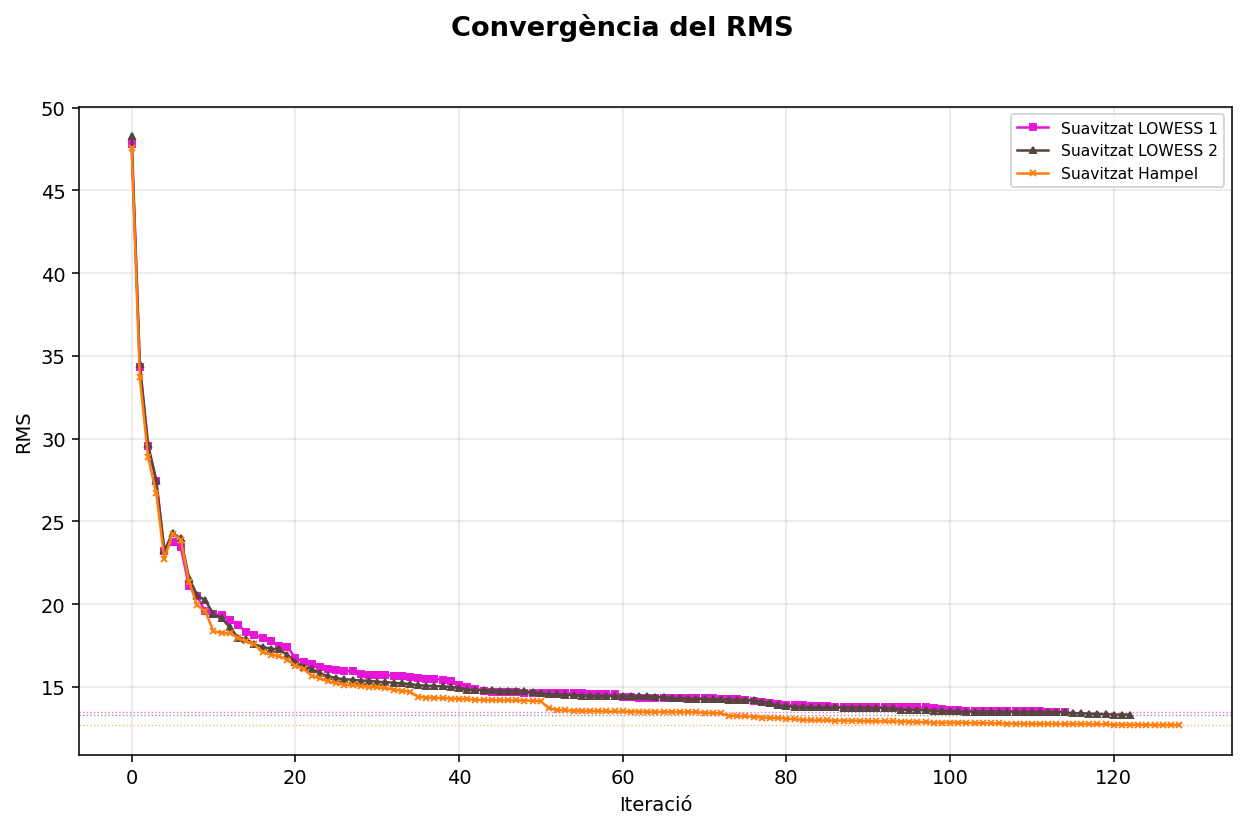
\includegraphics[width=\linewidth]{rms_comparison_smooth.png}
    \small RMS
  \end{minipage}\hfill
  \begin{minipage}[t]{0.32\textwidth}
    \centering
    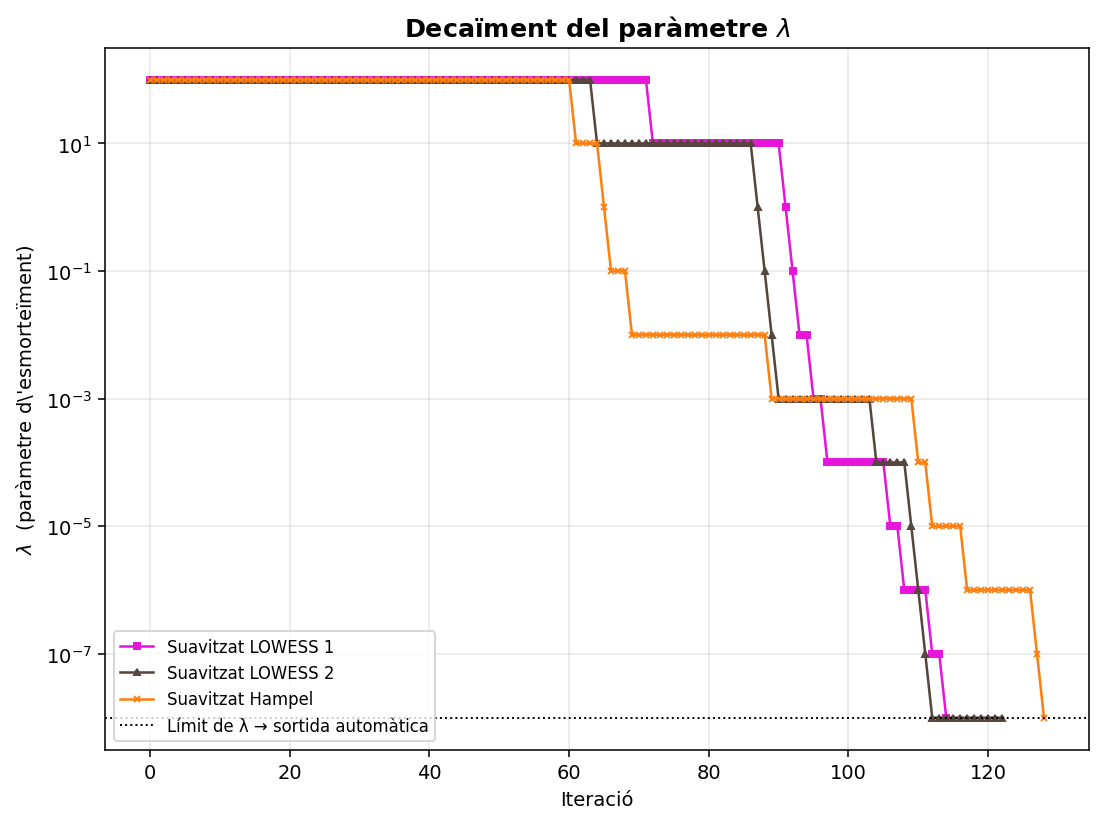
\includegraphics[width=\linewidth]{lambda_decay_smooth.png}
    \small Regularització $\lambda$
  \end{minipage}\hfill
  \begin{minipage}[t]{0.32\textwidth}
    \centering
    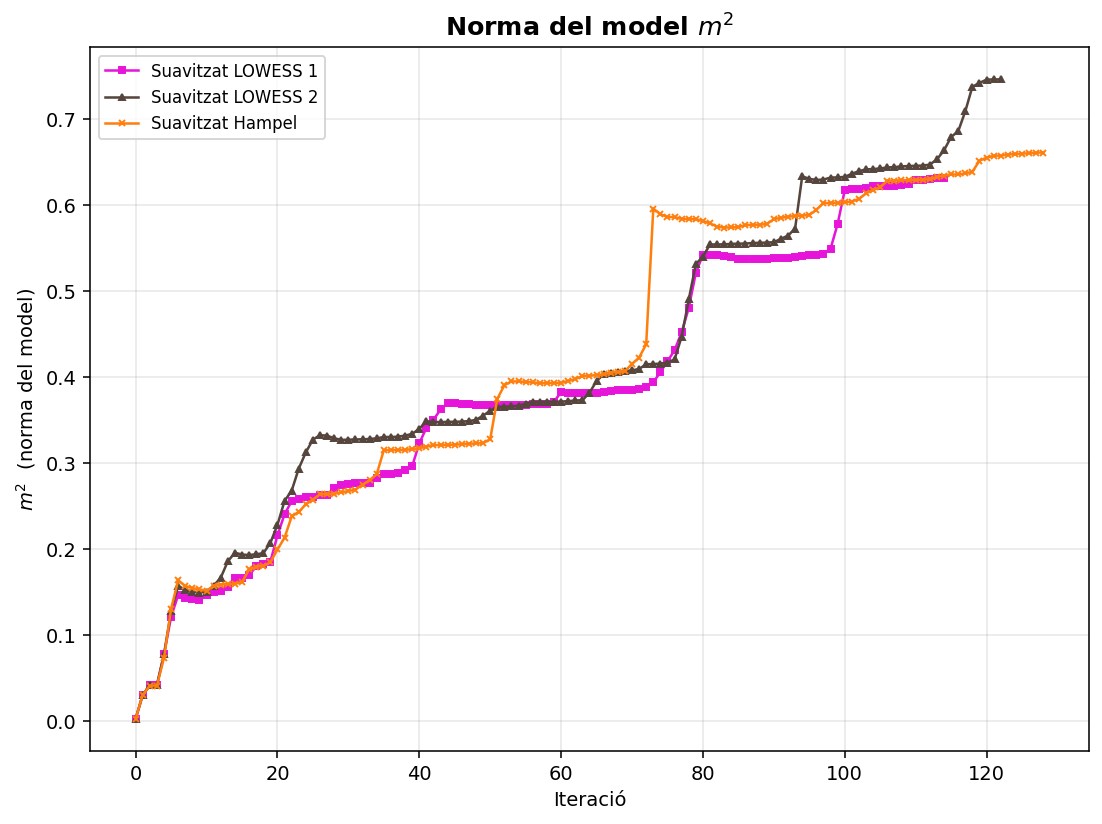
\includegraphics[width=\linewidth]{model_norm_smooth.png}
    \small Norma del model $m^2$
  \end{minipage}
  \caption{Evolució completa de l'RMS, del paràmetre de regularització i de la norma del model per a tots els assaigs.}
  \label{fig:annex-grafs-smooth}
\end{figure}

\section{Paràmetres dels suavitzats}
\begin{table}[htbp]
  \centering
  \footnotesize
  \setlength{\tabcolsep}{5pt}
  \begin{tabular}{l r r r r}
    \toprule
    Assaig & Iter. & RMS ini. & RMS fin. & $m^2_{\mathrm{fin}}$ \\
    \midrule
    Suavitzat LOWESS 1 & 115 & 47.78 & 13.51 & 0.631 \\
    Suavitzat LOWESS 2 & 123 & 48.27 & 13.33 & 0.746 \\
    Suavitzat Hampel & 129 & 47.58 & 12.69 & 0.661 \\
    \bottomrule
  \end{tabular}
  \caption{Inversions ModEM NLCG amb depuració algorítmica dels registres. Els
    algorismes actuen només sobre les components antidiagonals; les diagonals
    conserven l'error natiu.}
  \label{tab:modem_suavitzats}
\end{table}

\section{Comparació dels talls horitzontals amb el model de referència}
\label{annex:comparacio-talls-arango}

\begin{figure}[H]
  \centering
  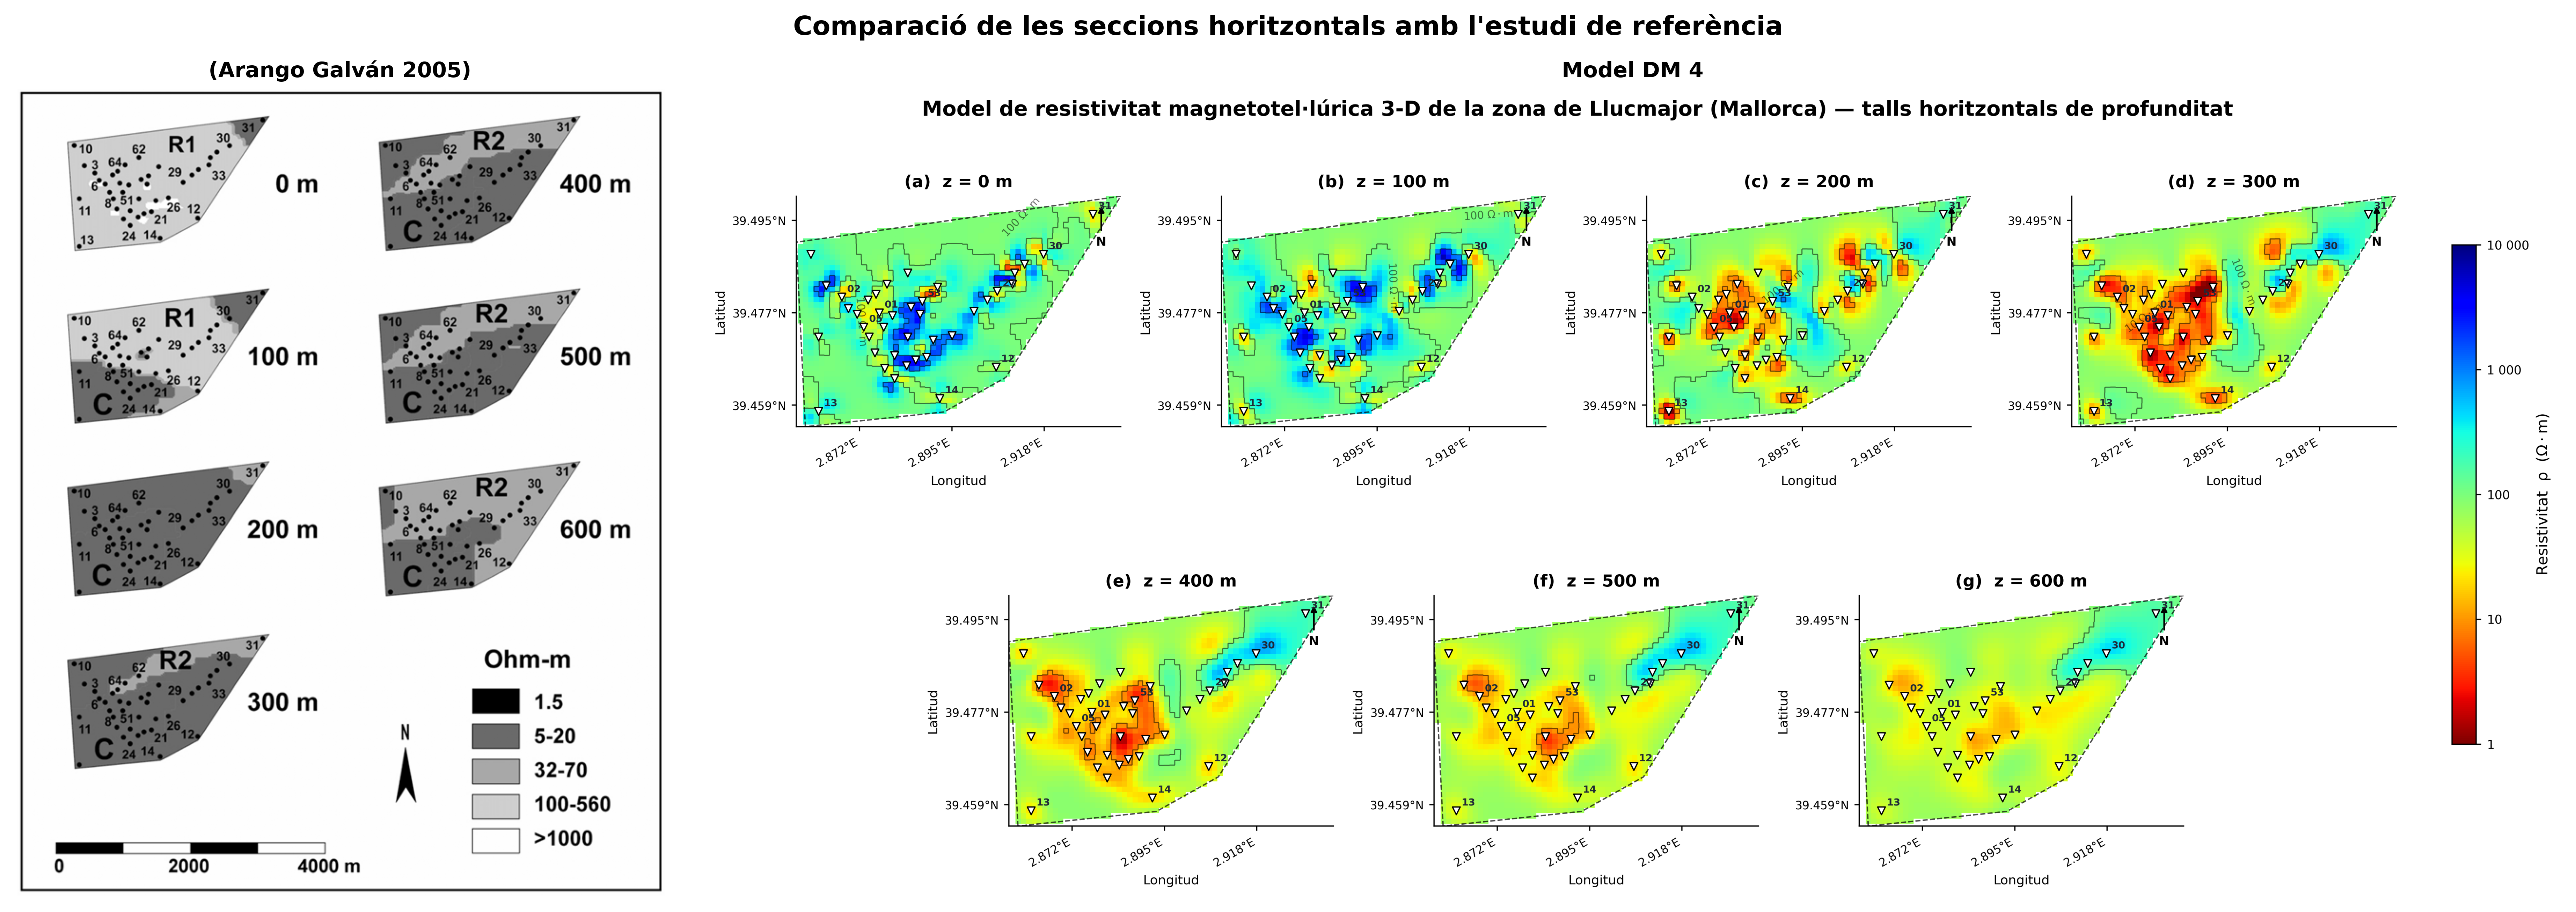
\includegraphics[width=\textwidth,height=0.23\textheight,keepaspectratio]{compare_depth_slices_arango_figure.png}
  \caption{Comparació dels talls horitzontals del model DM 4 amb els resultats de \citet{arango2005}.}
  \label{fig:annex-comparacio-talls-arango}
\end{figure}
\endgroup

\clearpage

\section{Ajust de $\rho_a$ i $\phi$}
\label{annex:ajust-dades-fase}

\begingroup
\setstretch{1}
\captionsetup{font=small,skip=3pt}
\setlength{\tabcolsep}{0pt}
\begin{figure}[H]
  \centering
  \begin{tabular}{@{}ccccc@{}}
    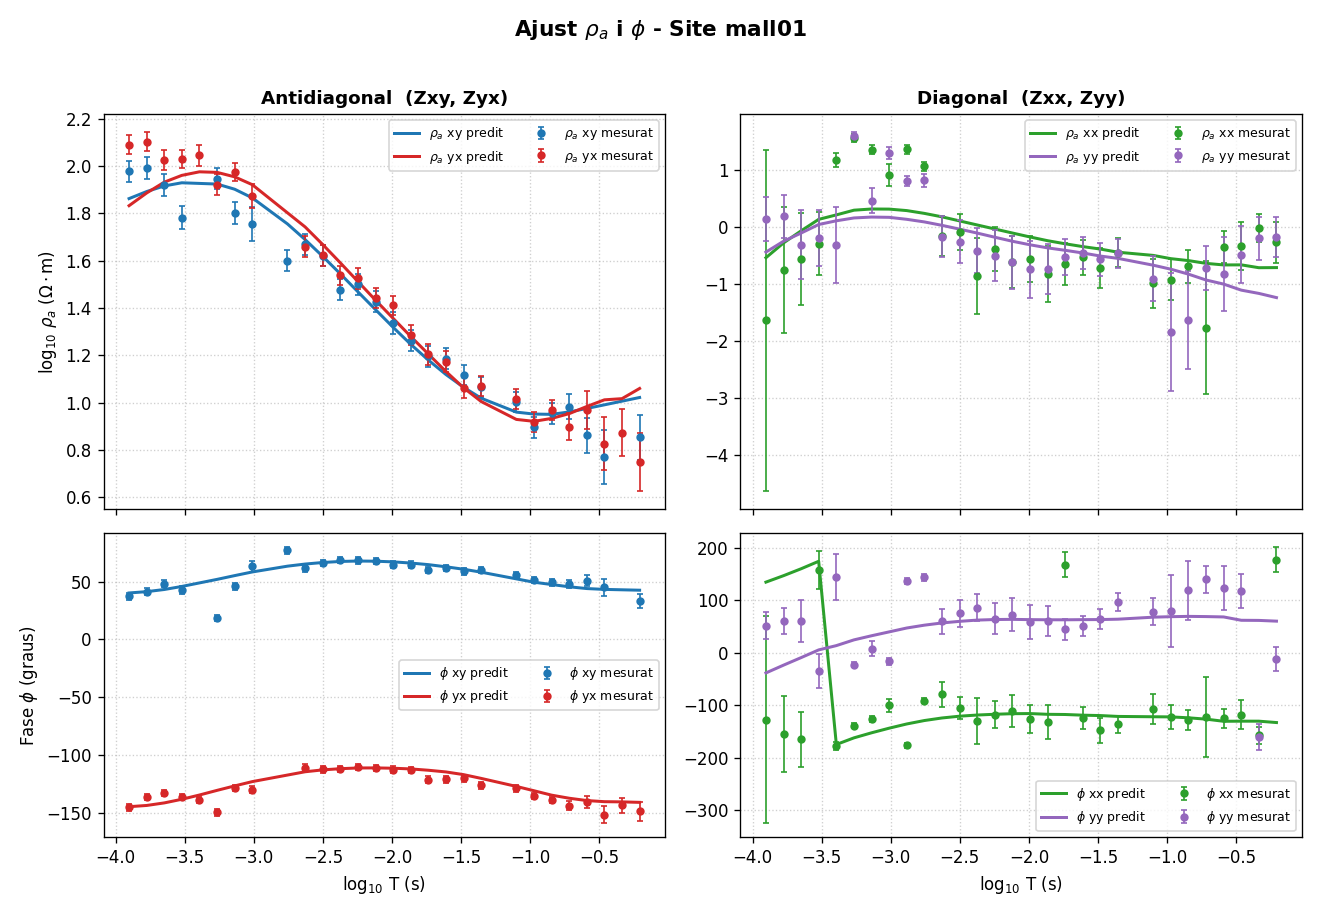
\includegraphics[width=0.198\textwidth]{Ajust_Dades_Fase/mall01f.png} &
    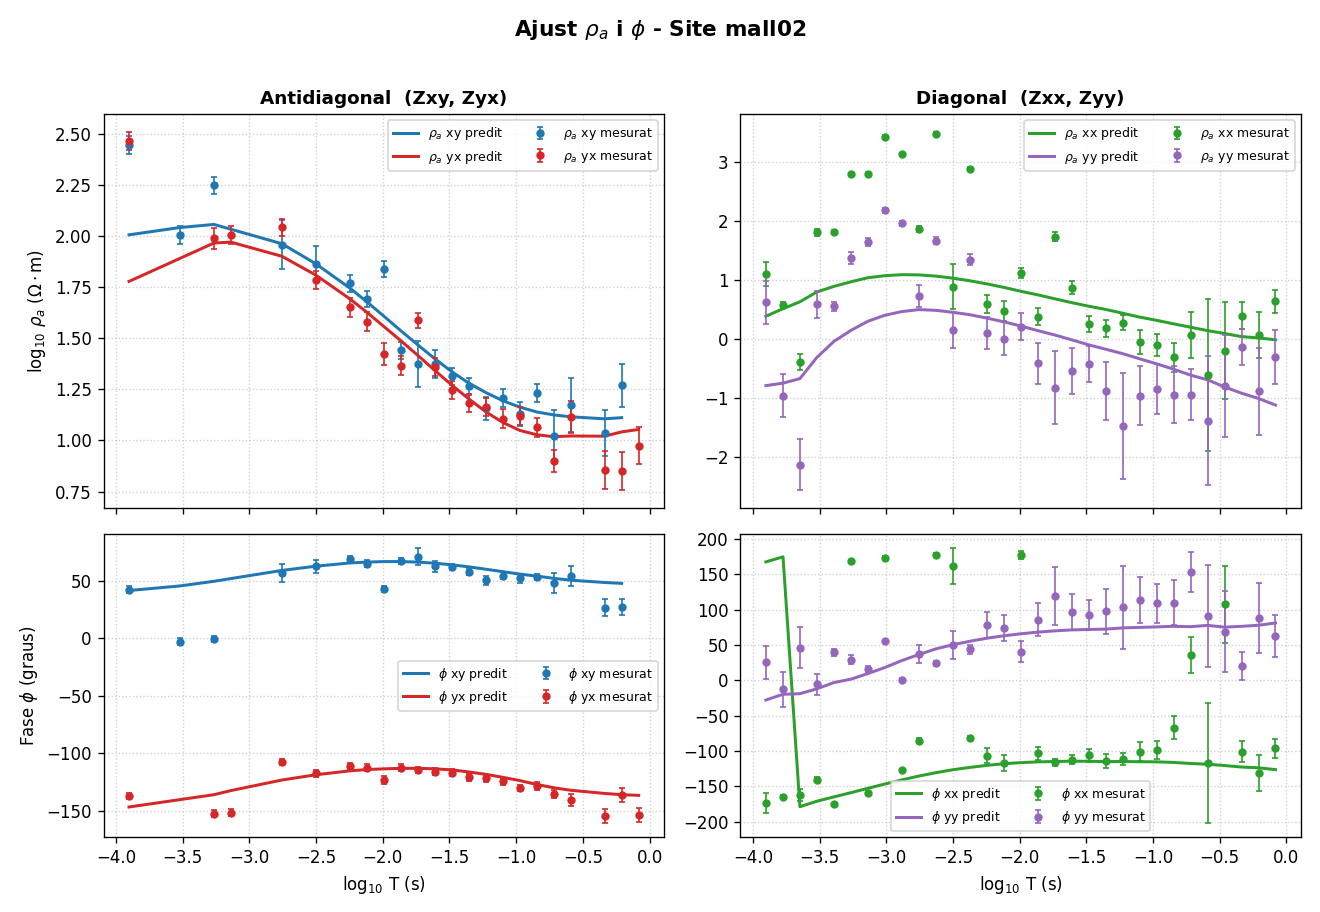
\includegraphics[width=0.198\textwidth]{Ajust_Dades_Fase/mall02f.png} &
    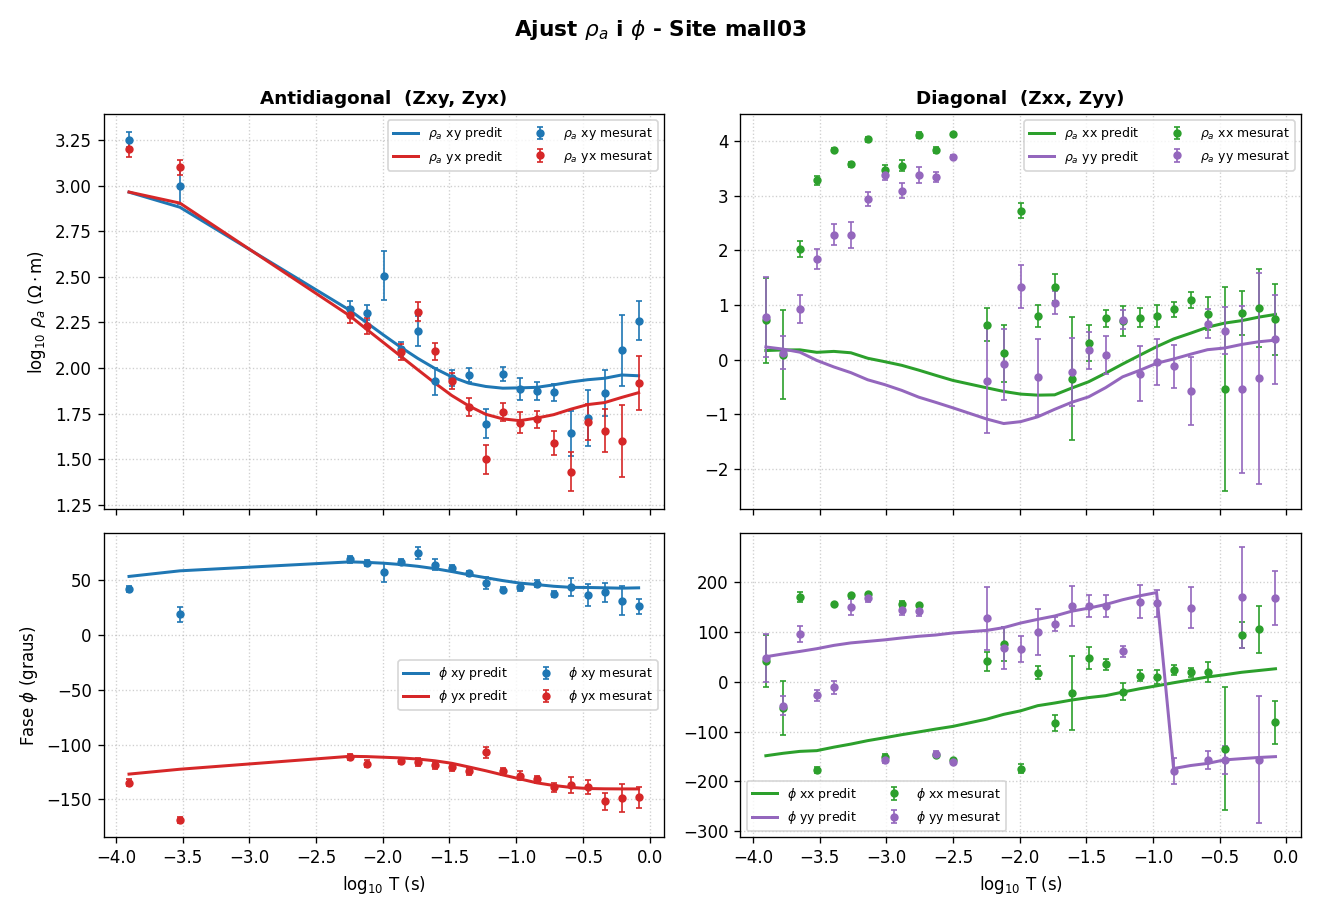
\includegraphics[width=0.198\textwidth]{Ajust_Dades_Fase/mall03f.png} &
    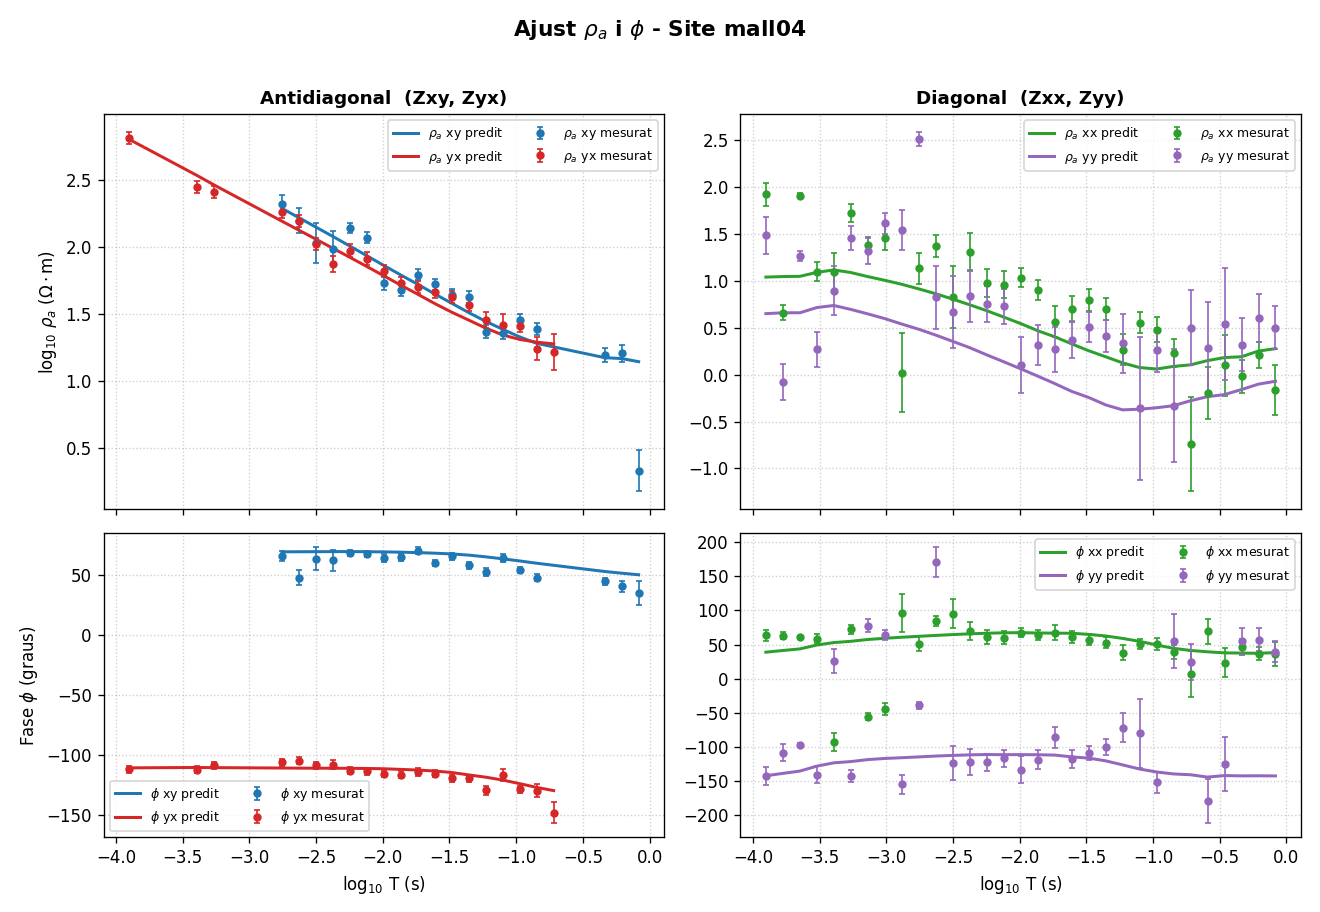
\includegraphics[width=0.198\textwidth]{Ajust_Dades_Fase/mall04f.png} &
    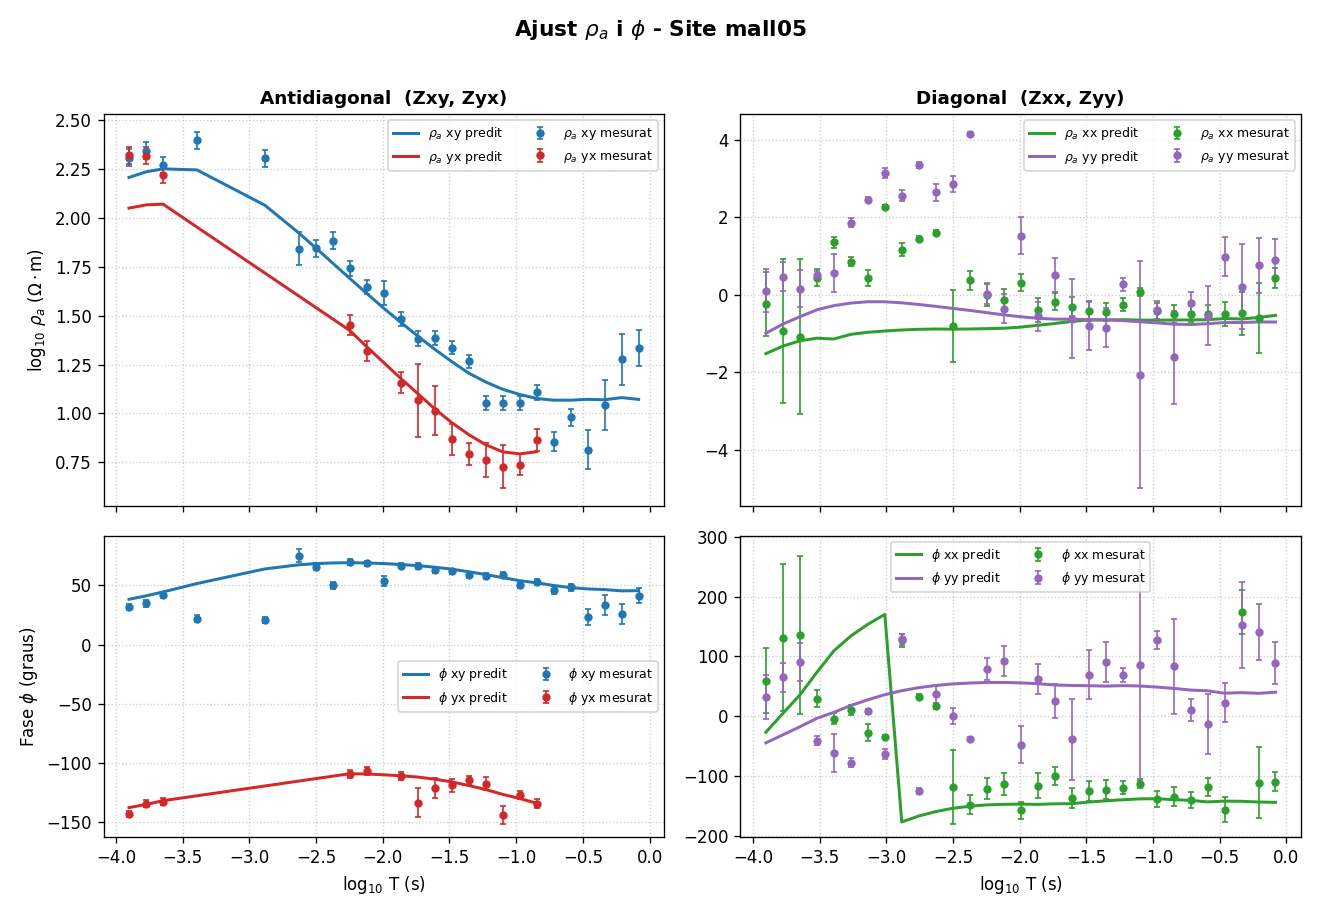
\includegraphics[width=0.198\textwidth]{Ajust_Dades_Fase/mall05f.png} \\[8pt]
    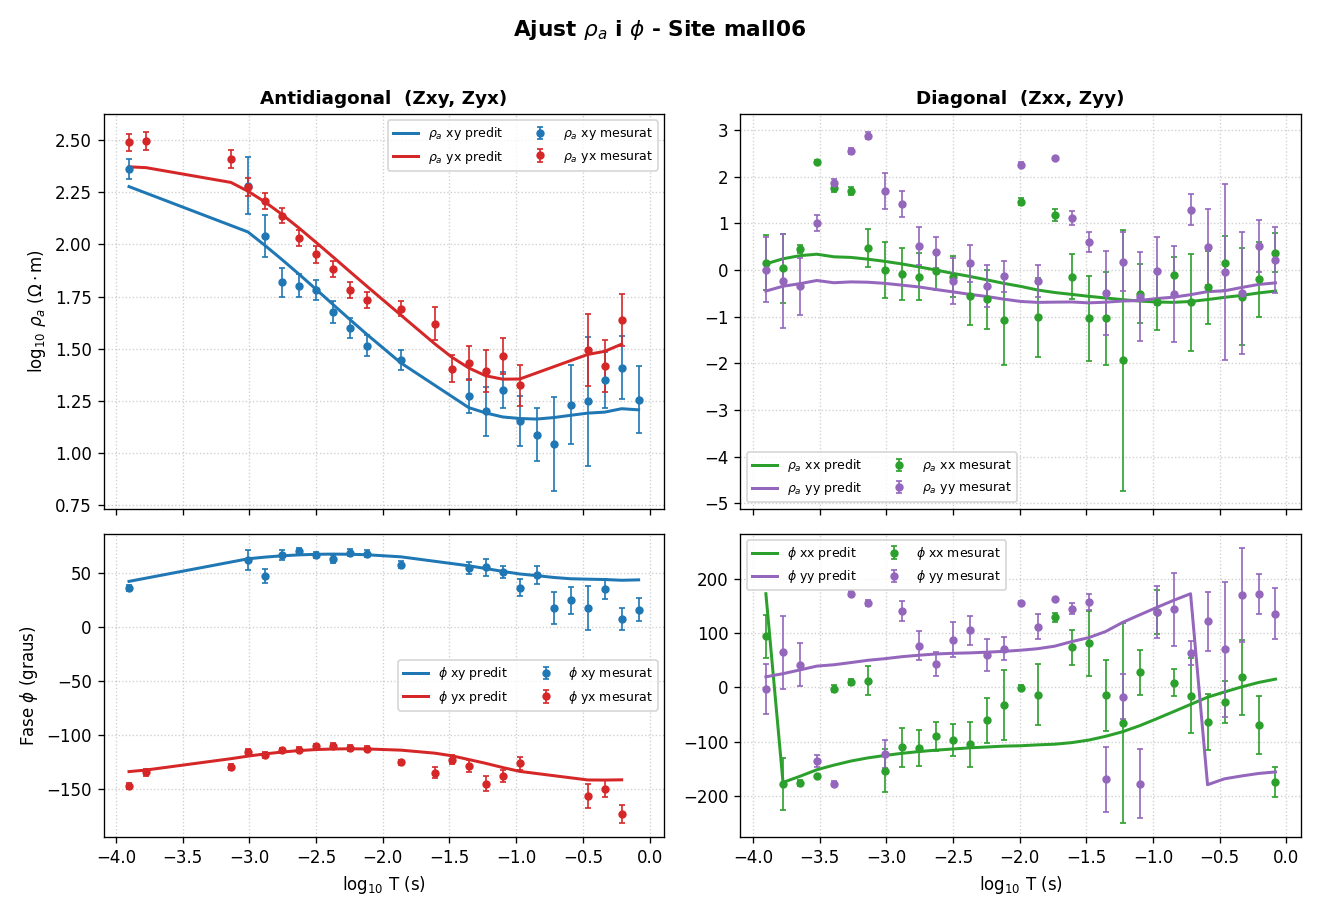
\includegraphics[width=0.198\textwidth]{Ajust_Dades_Fase/mall06f.png} &
    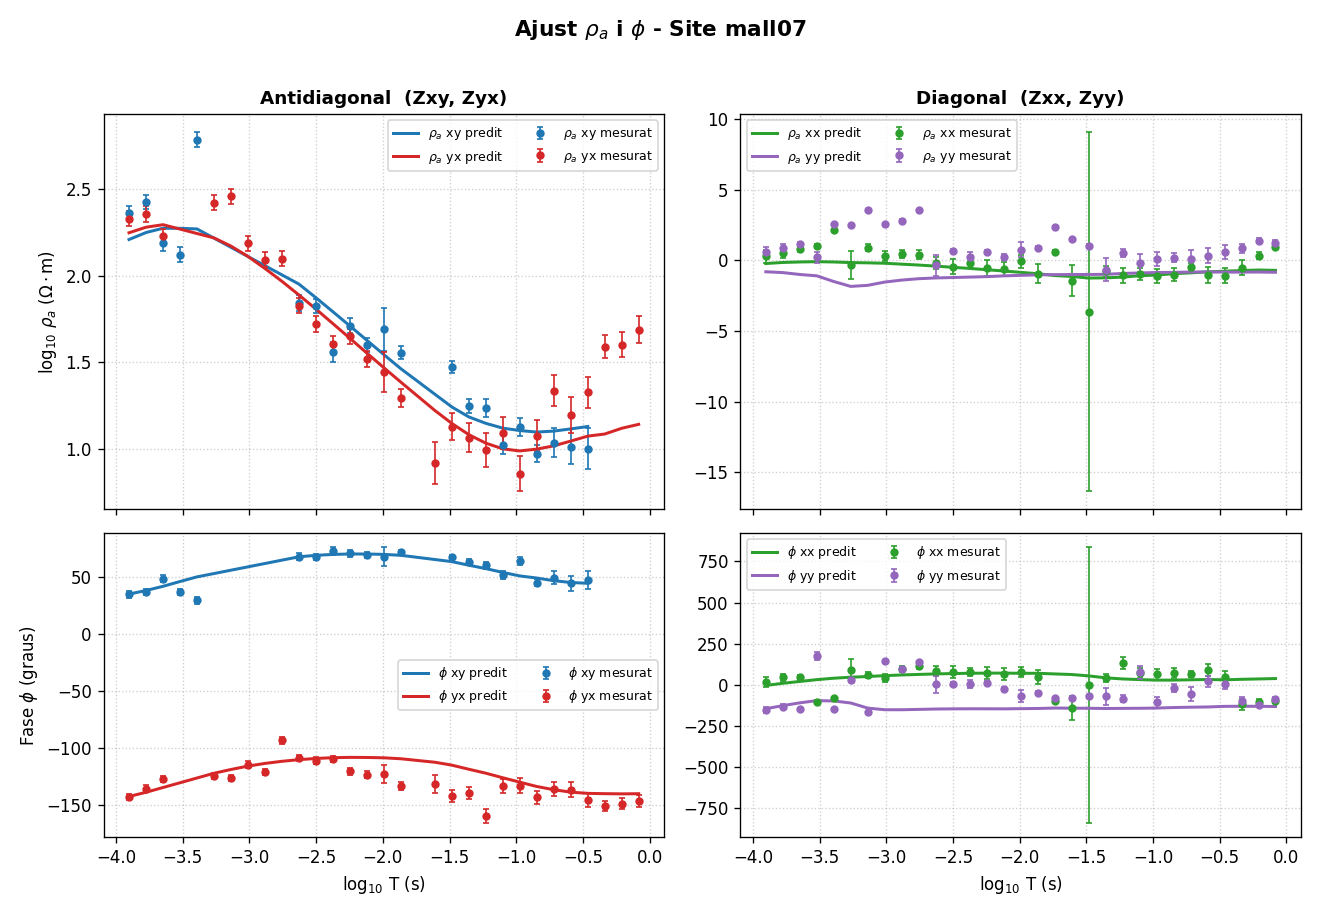
\includegraphics[width=0.198\textwidth]{Ajust_Dades_Fase/mall07f.png} &
    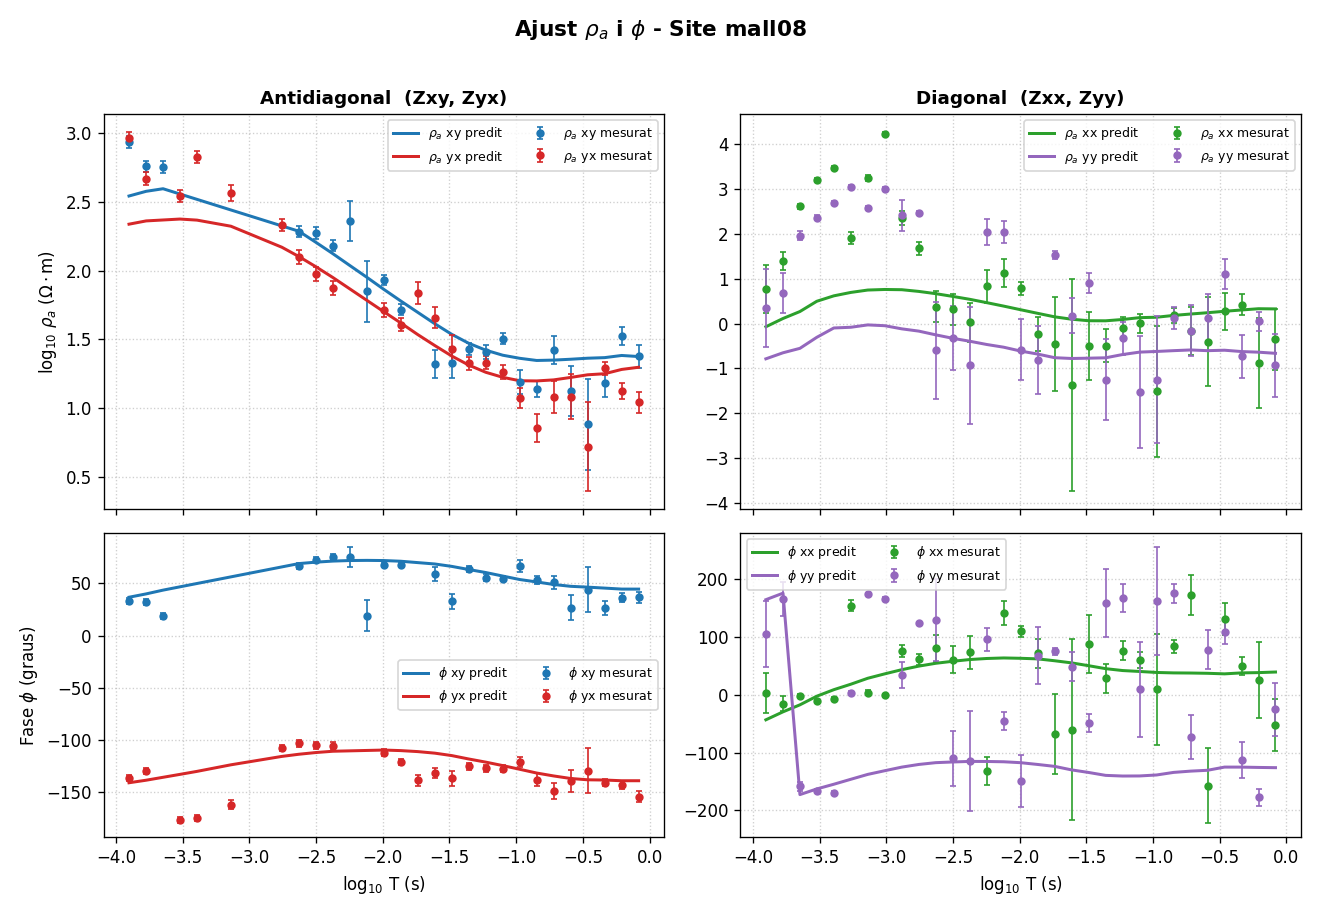
\includegraphics[width=0.198\textwidth]{Ajust_Dades_Fase/mall08f.png} &
    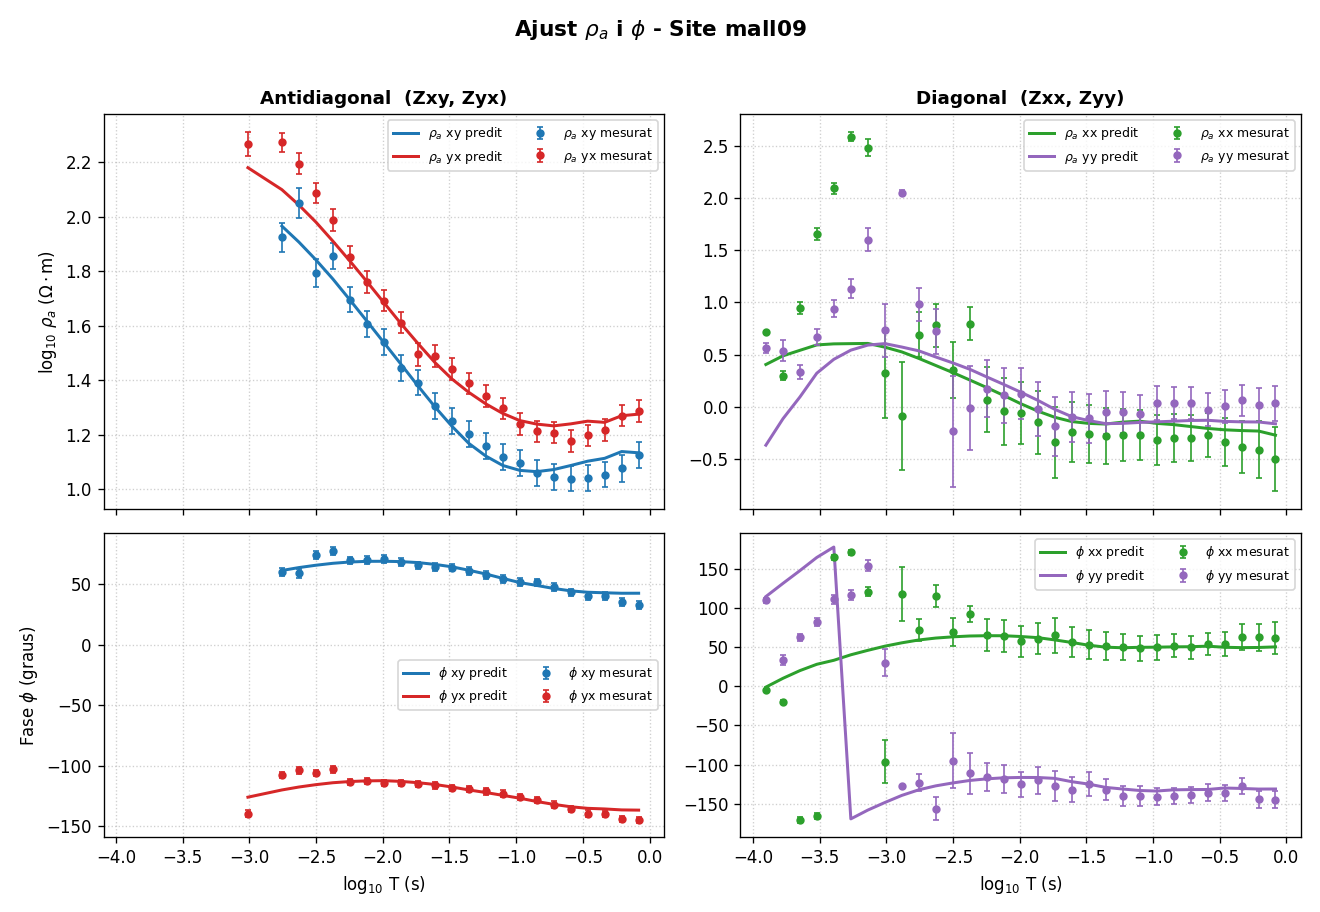
\includegraphics[width=0.198\textwidth]{Ajust_Dades_Fase/mall09f.png} &
    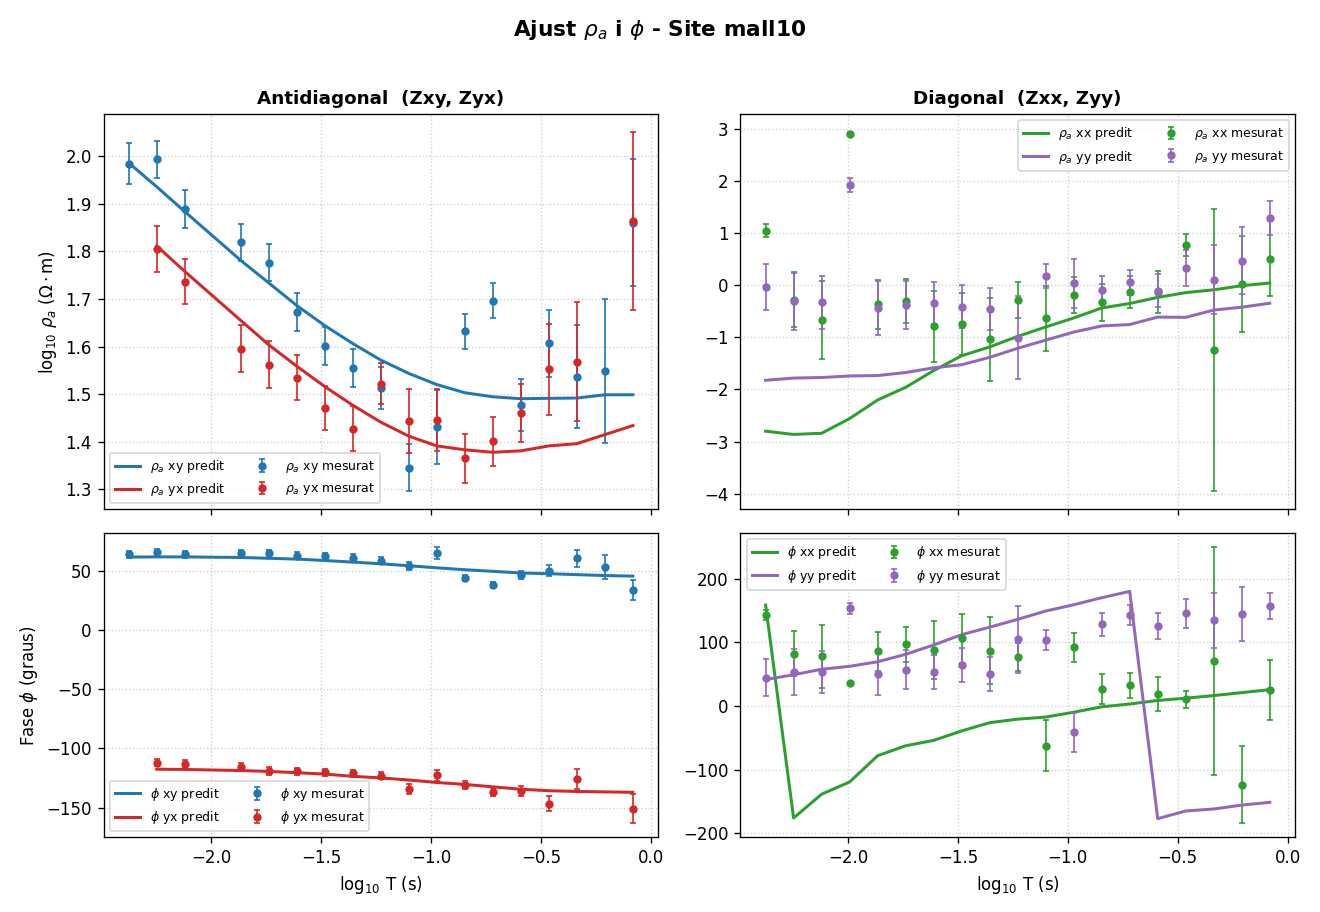
\includegraphics[width=0.198\textwidth]{Ajust_Dades_Fase/mall10f.png} \\[8pt]
    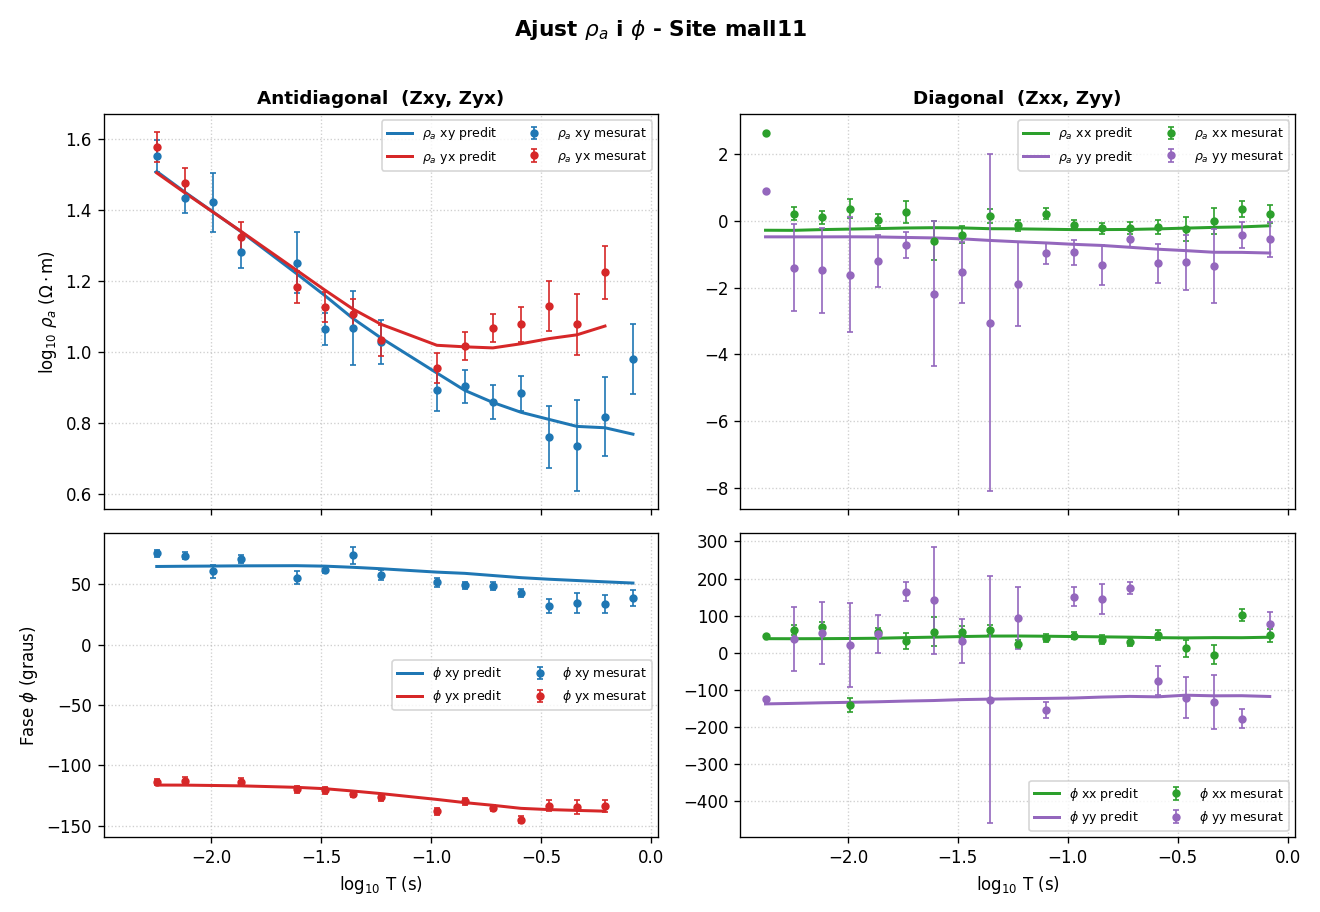
\includegraphics[width=0.198\textwidth]{Ajust_Dades_Fase/mall11f.png} &
    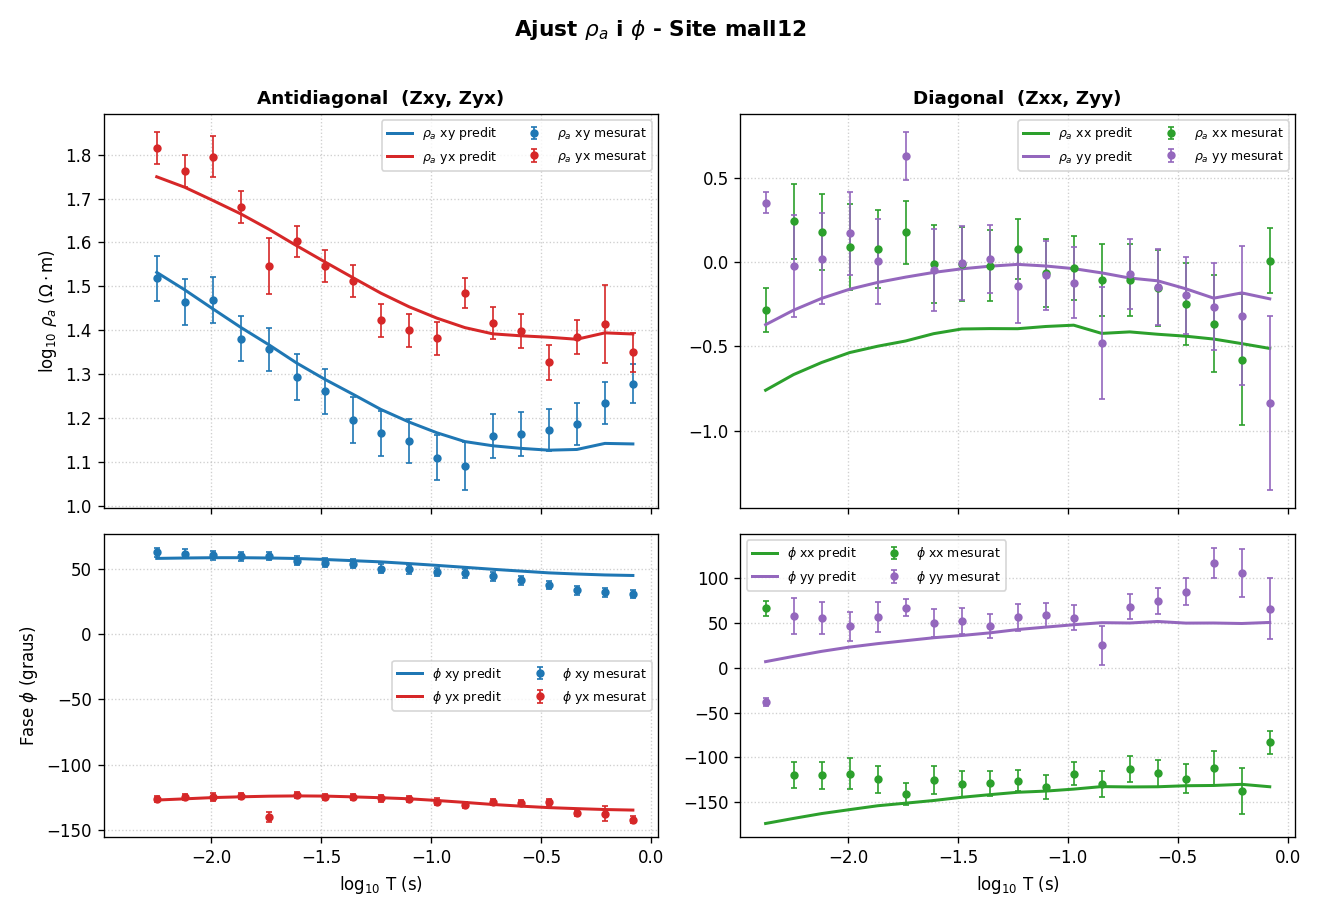
\includegraphics[width=0.198\textwidth]{Ajust_Dades_Fase/mall12f.png} &
    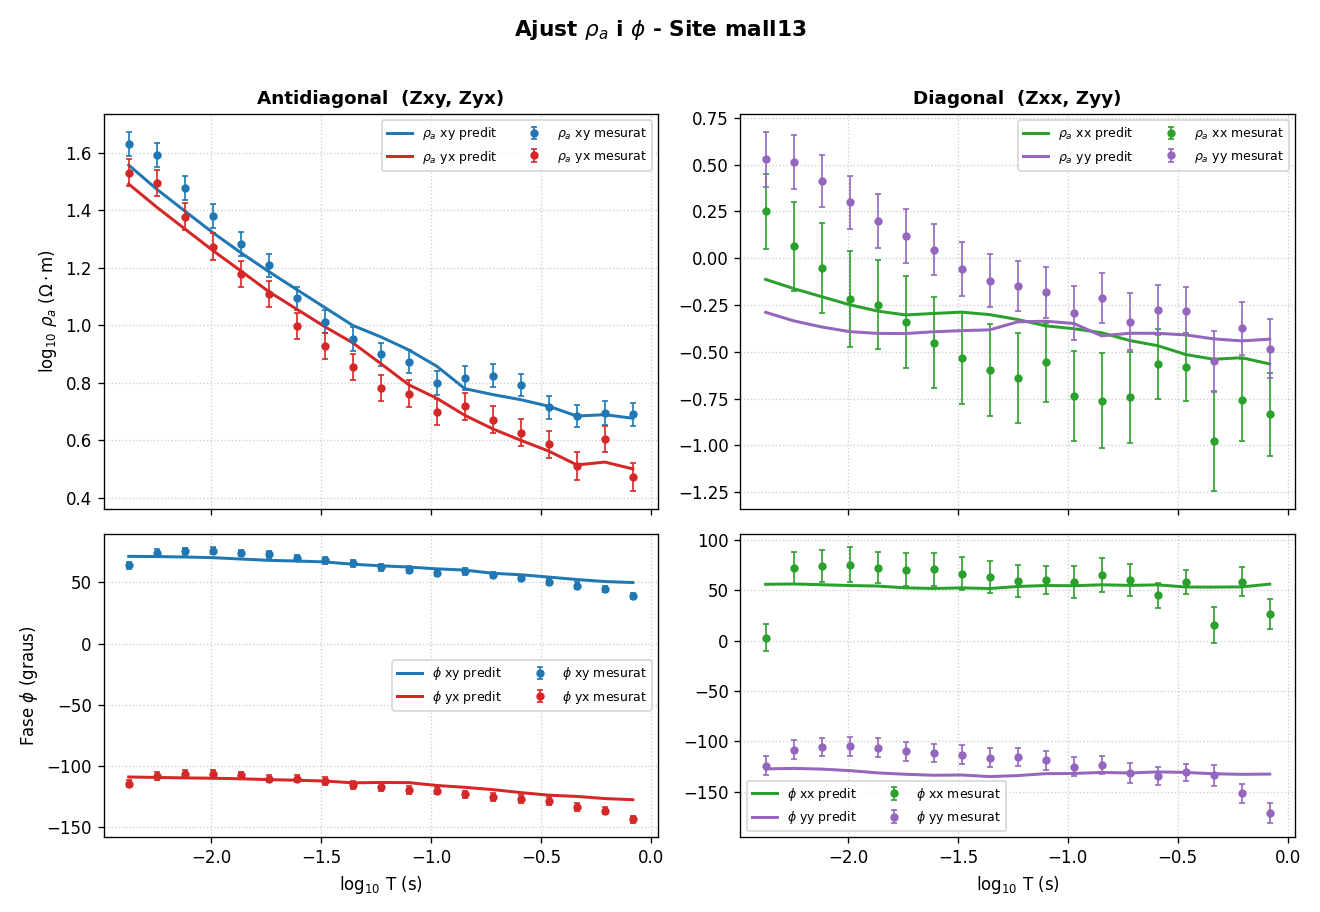
\includegraphics[width=0.198\textwidth]{Ajust_Dades_Fase/mall13f.png} &
    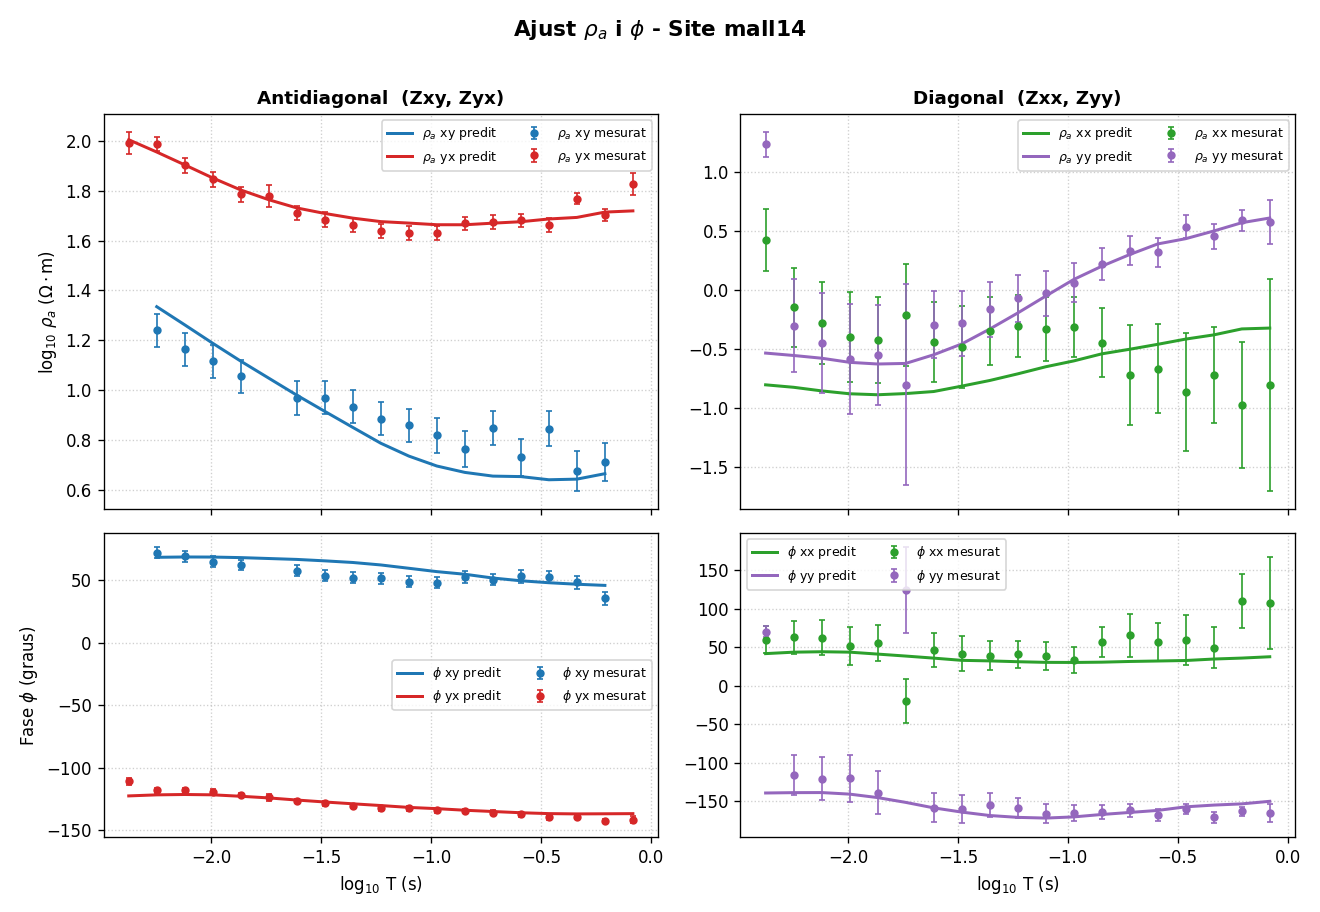
\includegraphics[width=0.198\textwidth]{Ajust_Dades_Fase/mall14f.png} &
    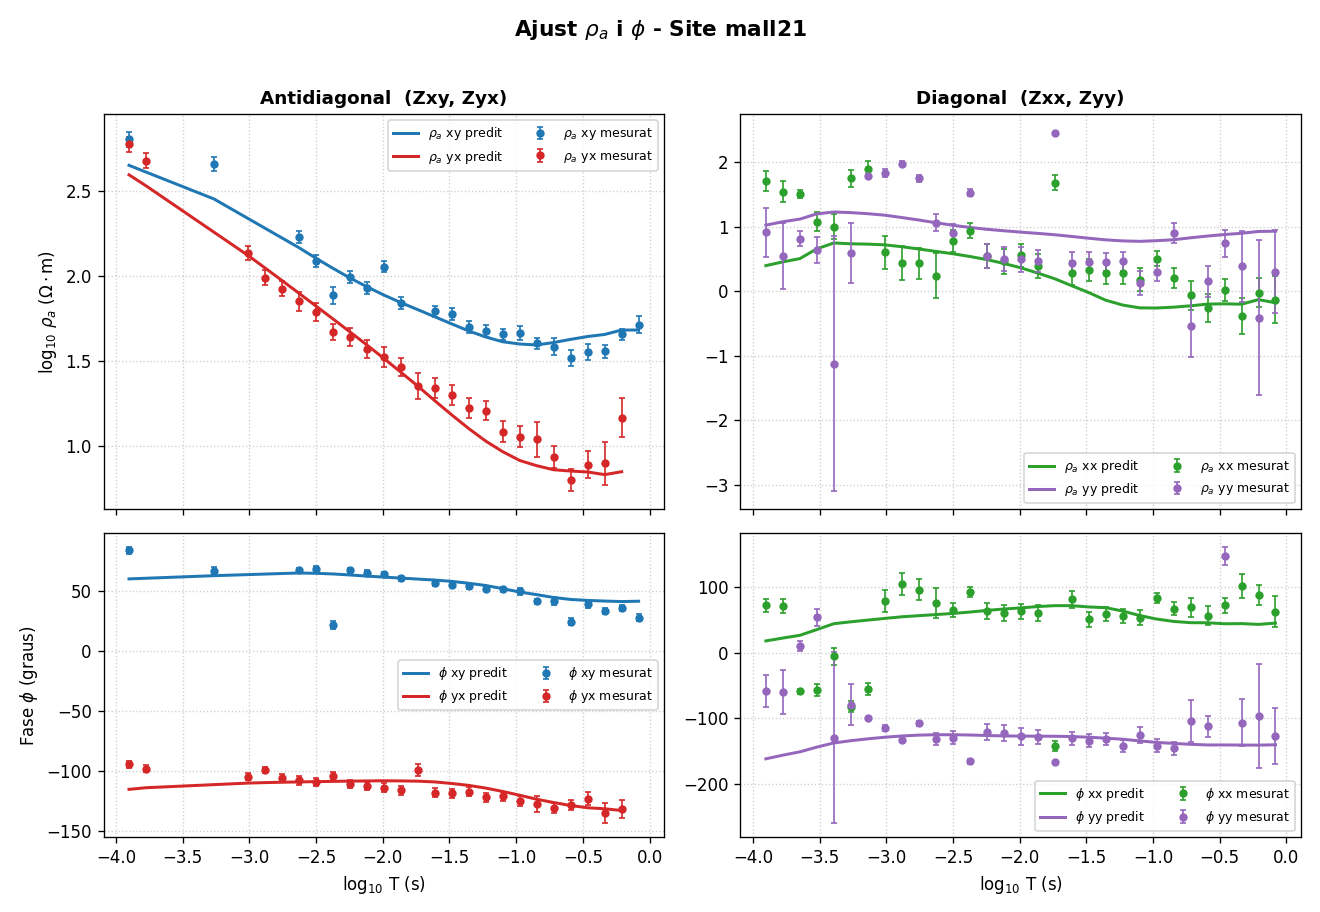
\includegraphics[width=0.198\textwidth]{Ajust_Dades_Fase/mall21f.png} \\[8pt]
    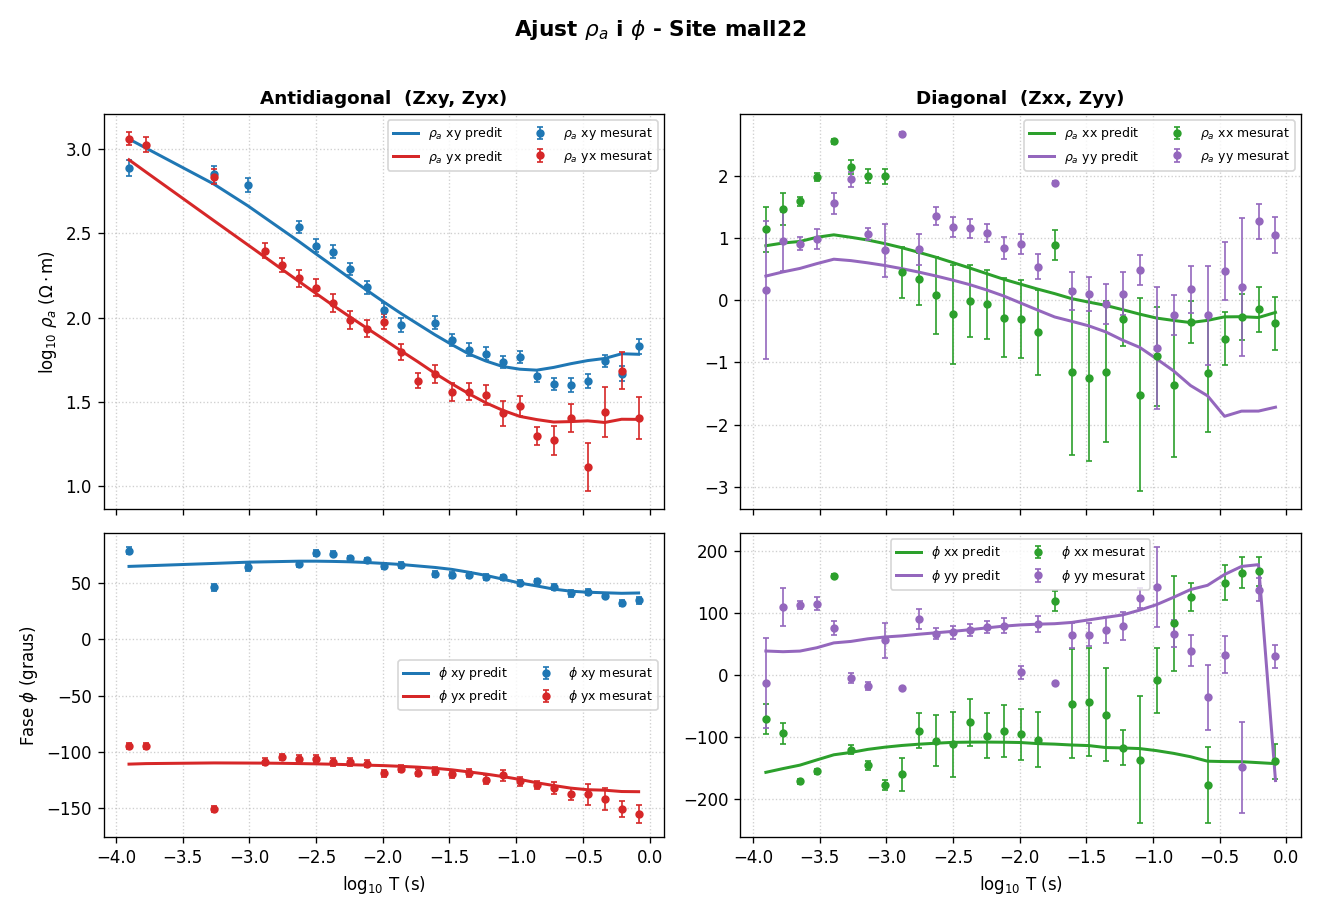
\includegraphics[width=0.198\textwidth]{Ajust_Dades_Fase/mall22f.png} &
    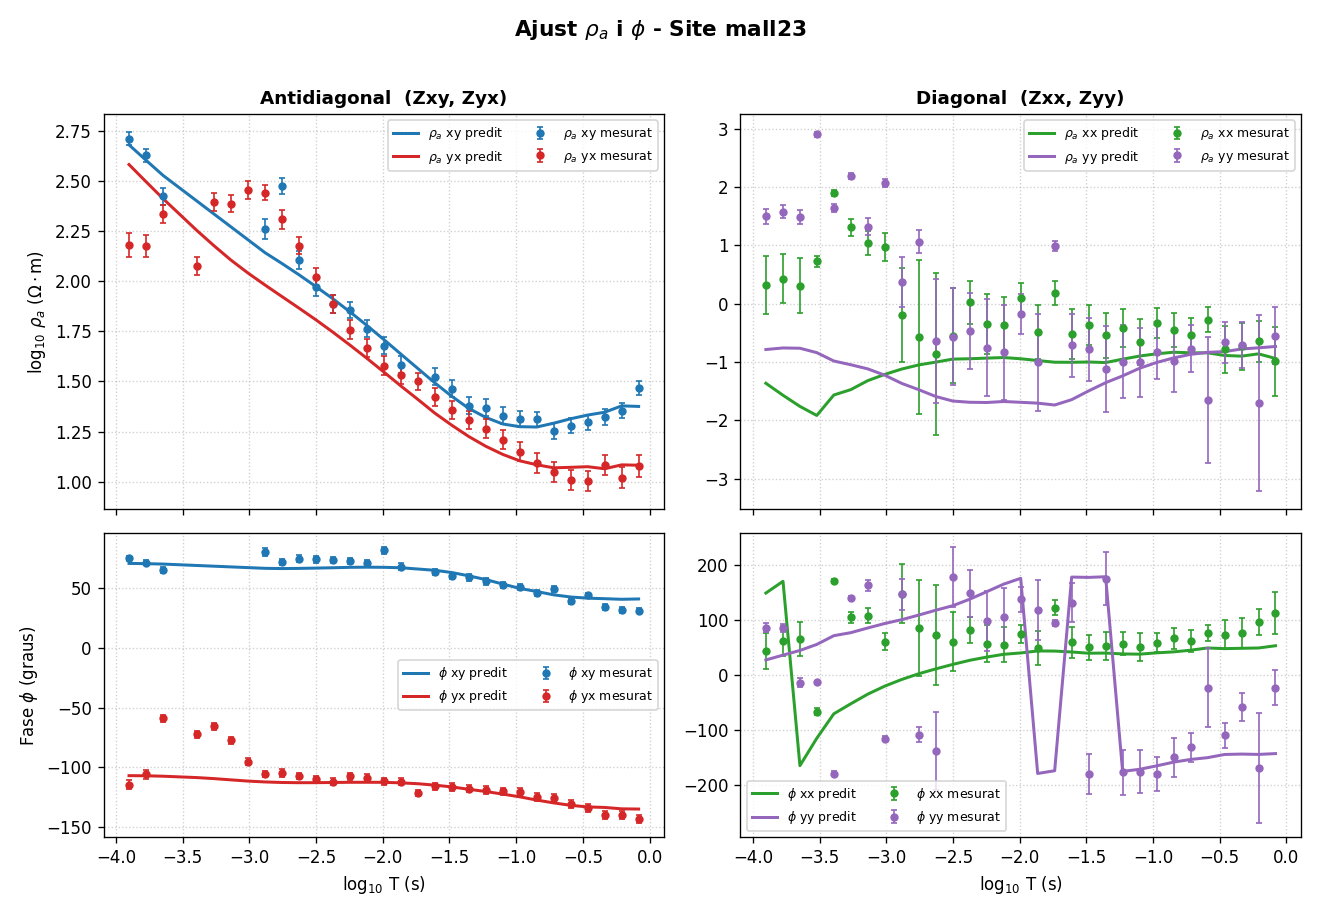
\includegraphics[width=0.198\textwidth]{Ajust_Dades_Fase/mall23f.png} &
    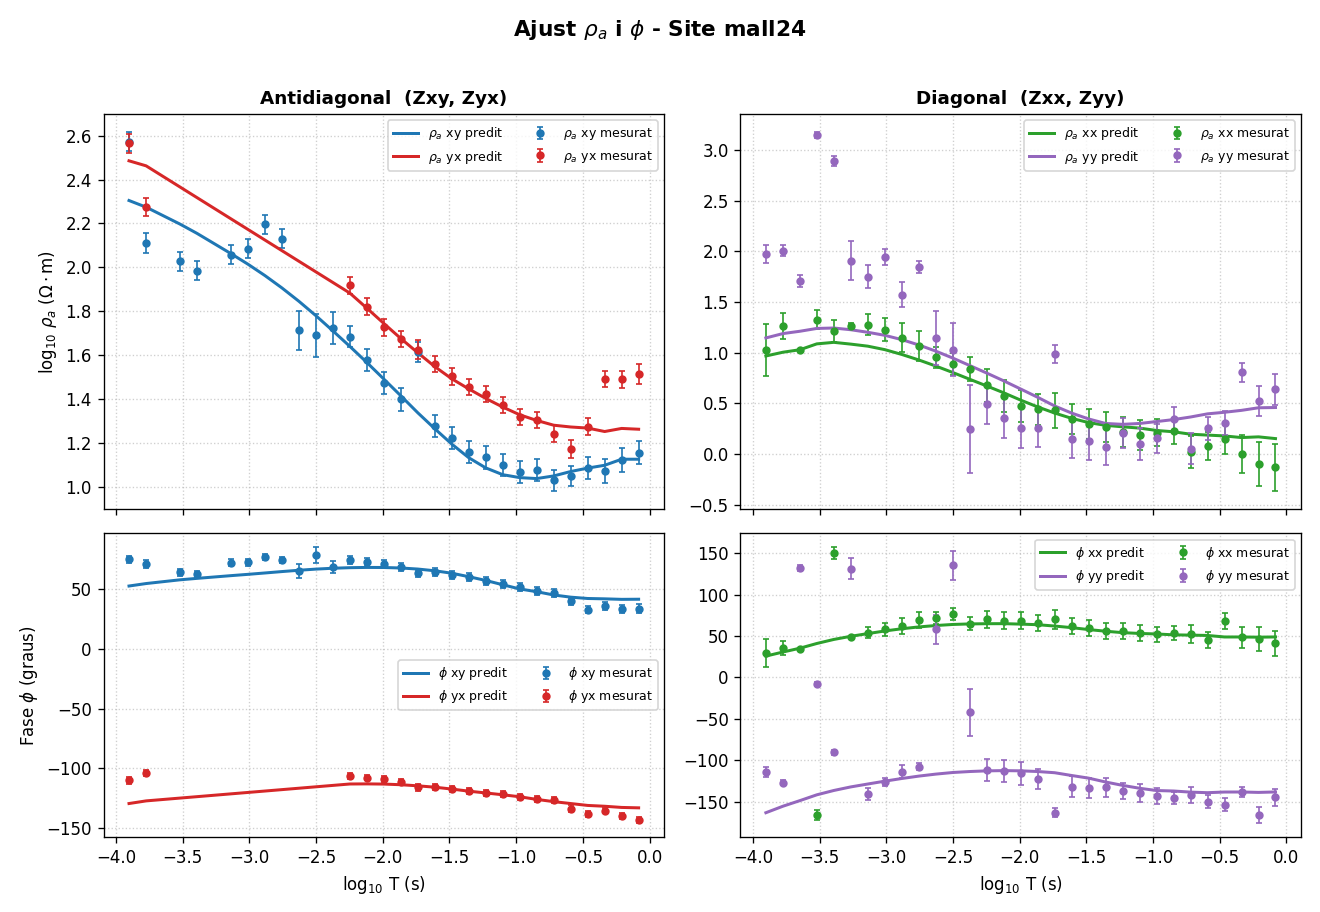
\includegraphics[width=0.198\textwidth]{Ajust_Dades_Fase/mall24f.png} &
    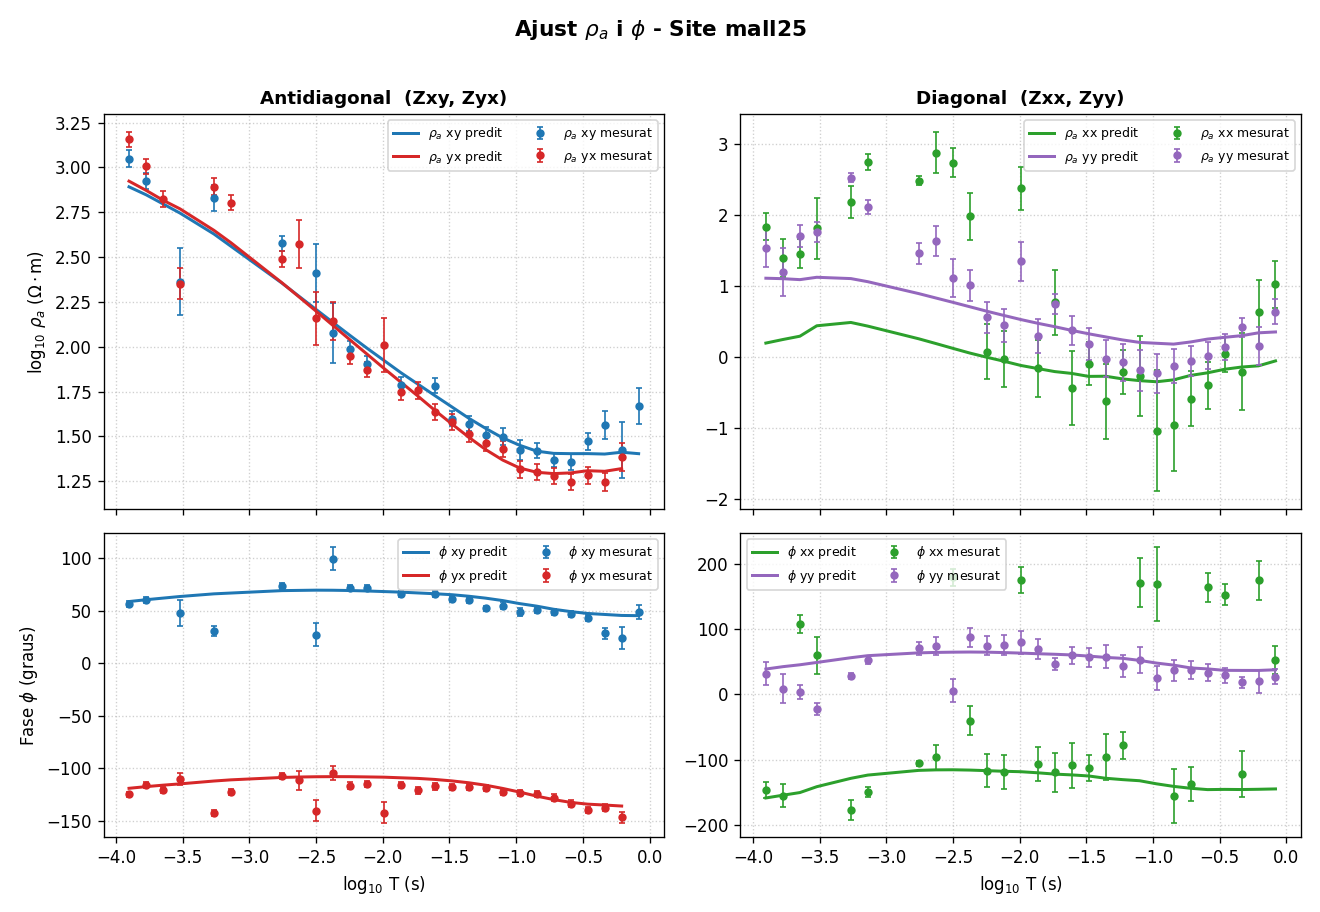
\includegraphics[width=0.198\textwidth]{Ajust_Dades_Fase/mall25f.png} &
    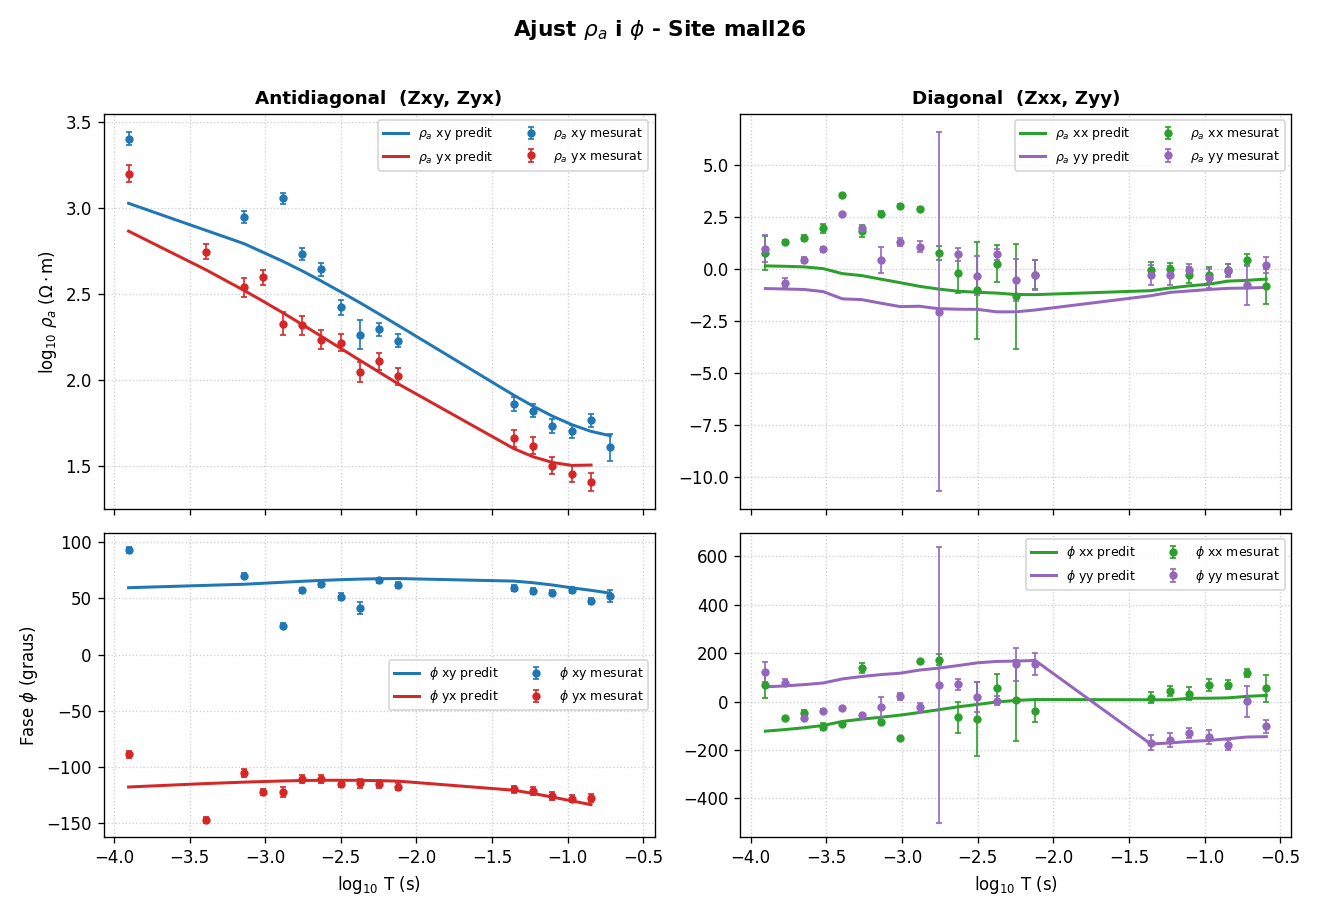
\includegraphics[width=0.198\textwidth]{Ajust_Dades_Fase/mall26f.png} \\[8pt]
    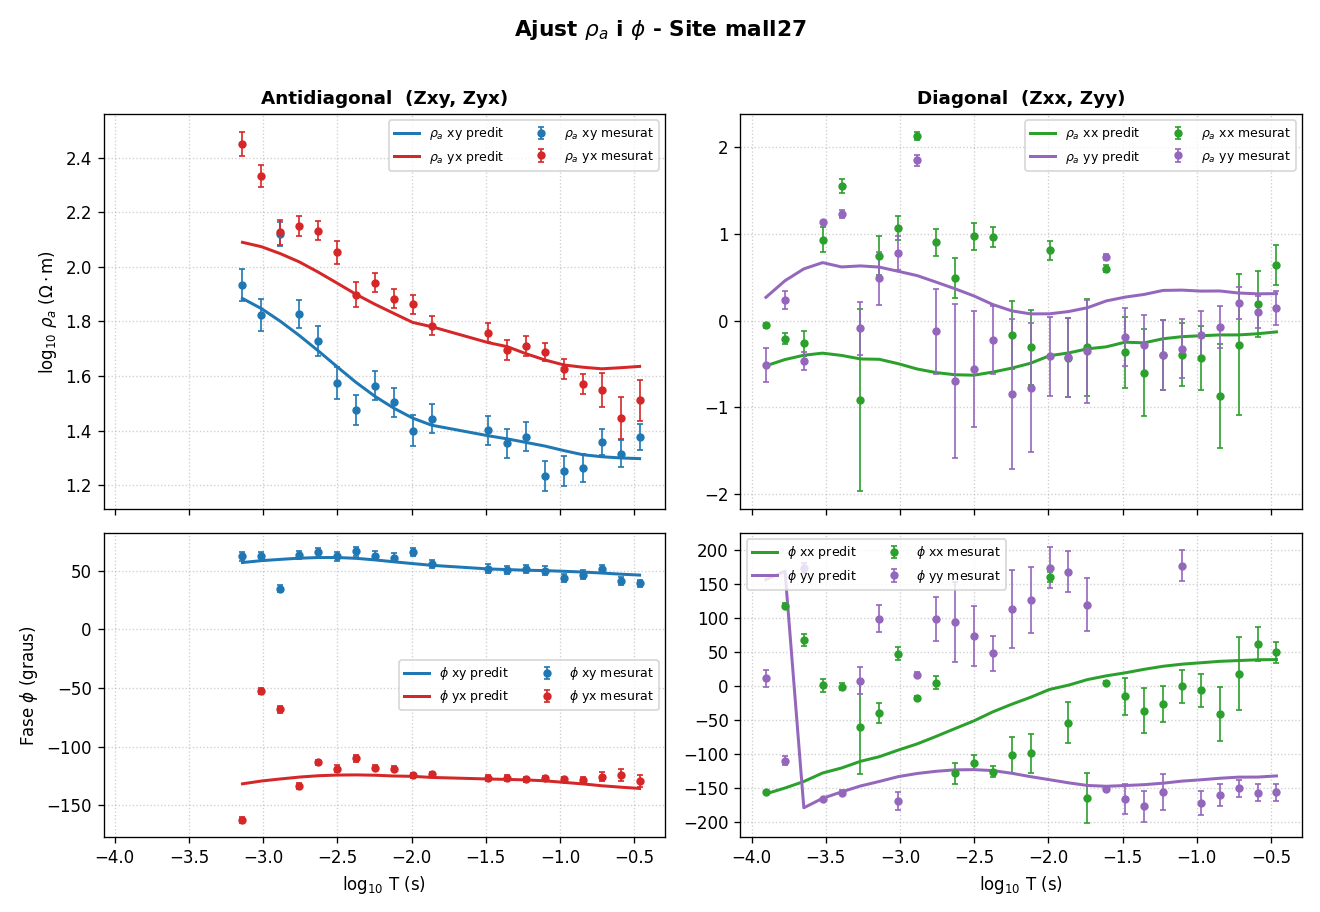
\includegraphics[width=0.198\textwidth]{Ajust_Dades_Fase/mall27f.png} &
    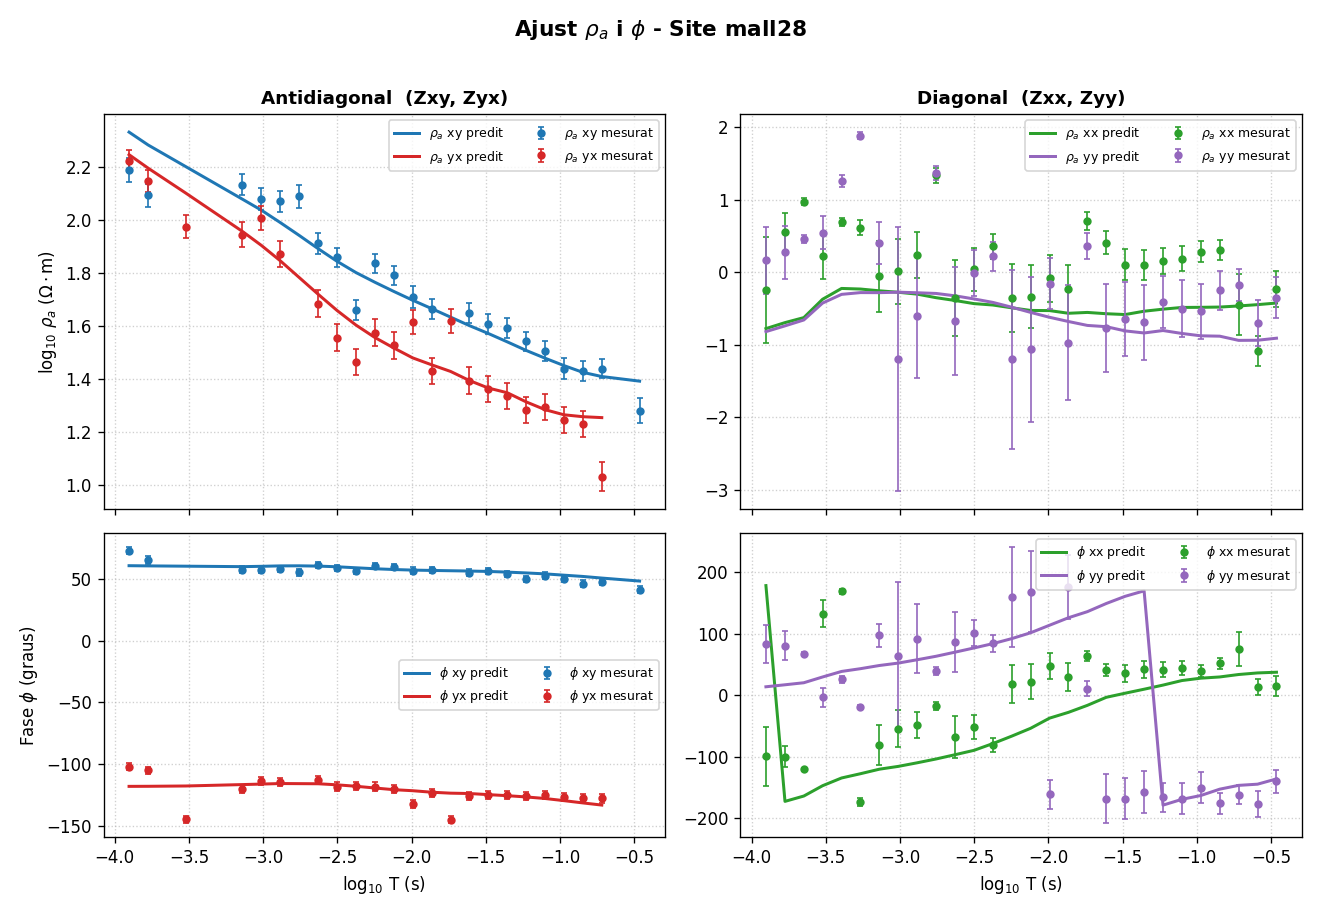
\includegraphics[width=0.198\textwidth]{Ajust_Dades_Fase/mall28f.png} &
    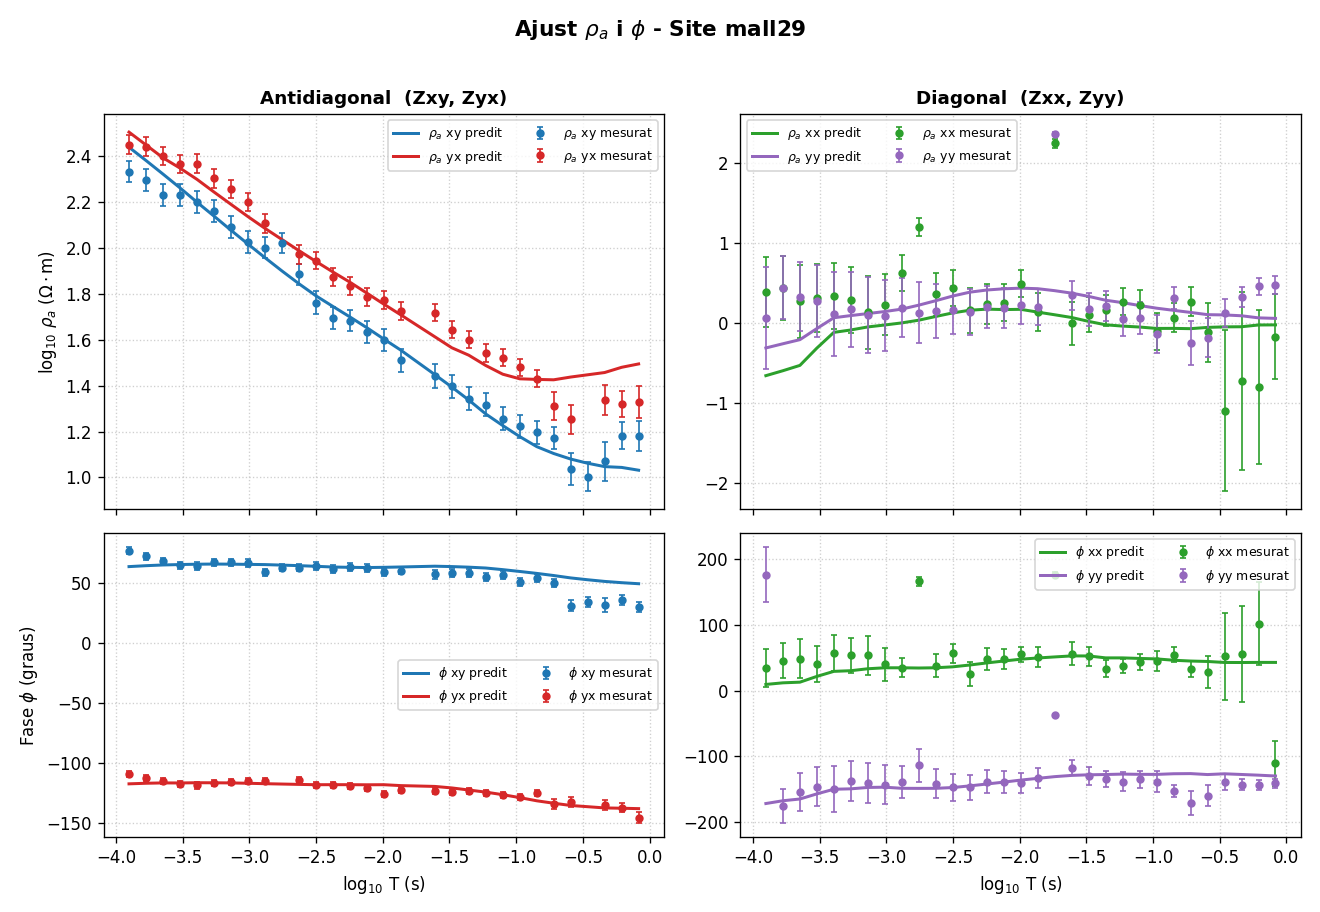
\includegraphics[width=0.198\textwidth]{Ajust_Dades_Fase/mall29f.png} &
    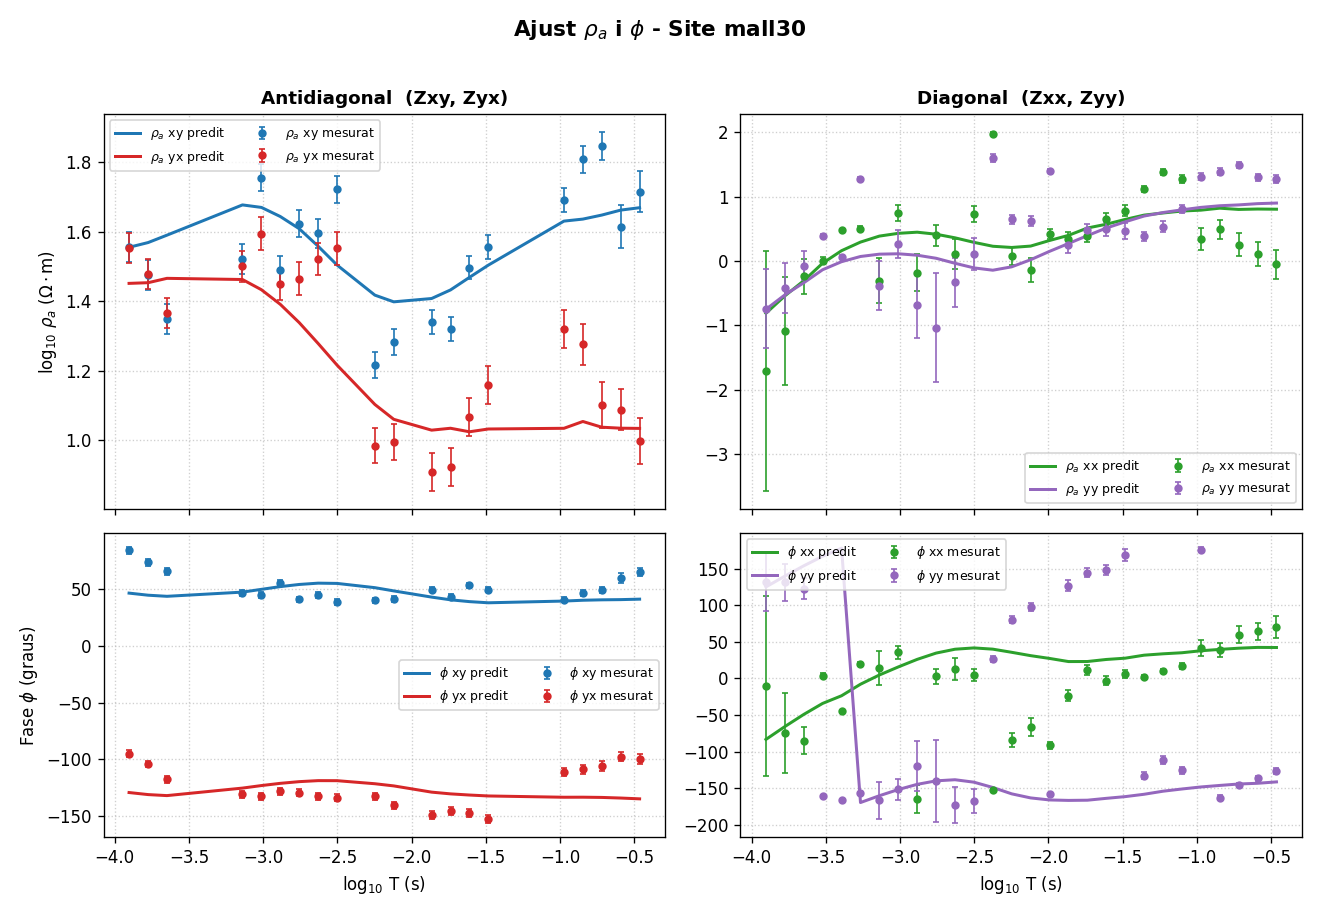
\includegraphics[width=0.198\textwidth]{Ajust_Dades_Fase/mall30f.png} &
    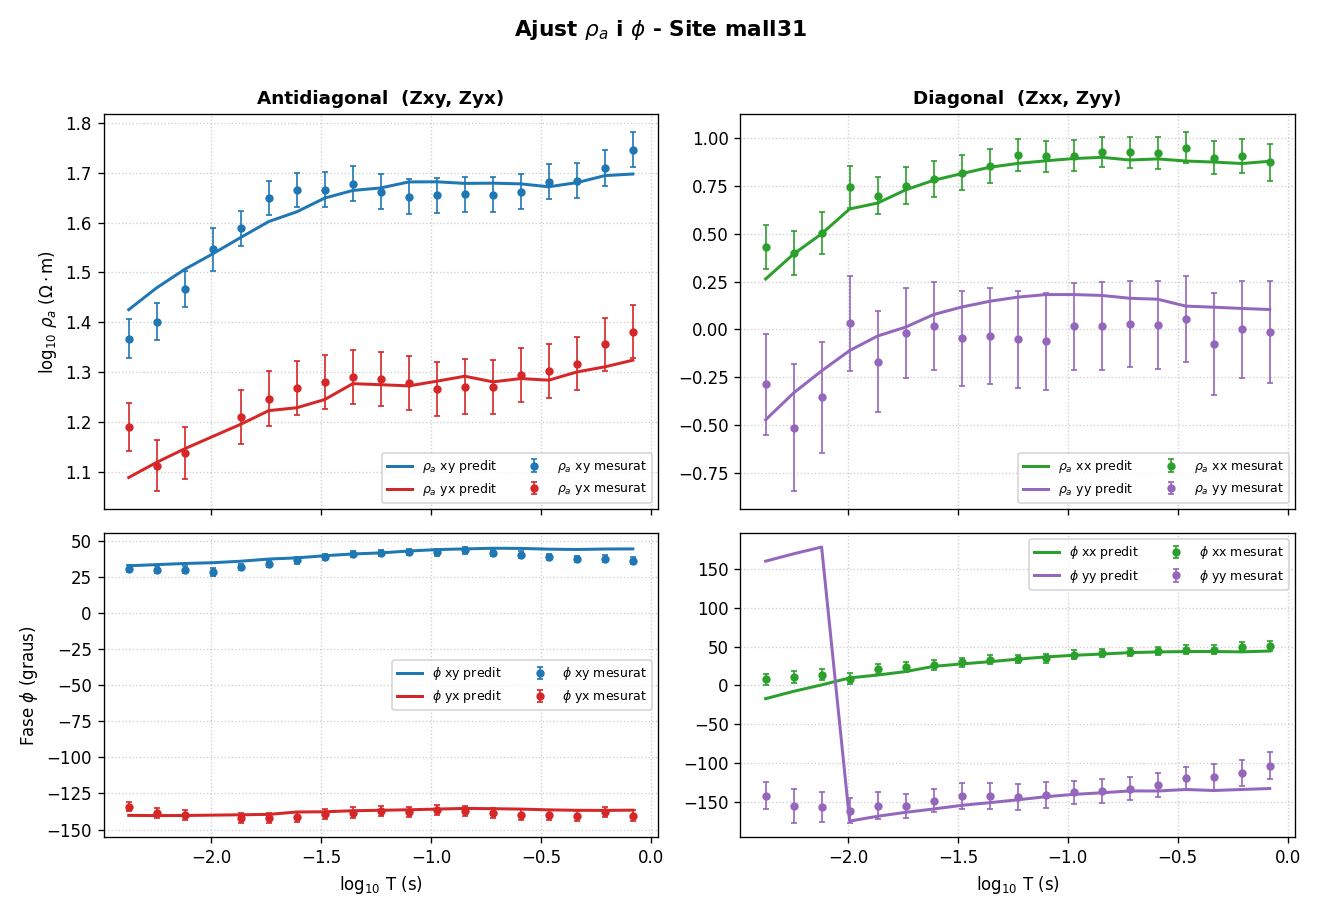
\includegraphics[width=0.198\textwidth]{Ajust_Dades_Fase/mall31f.png} \\[8pt]
    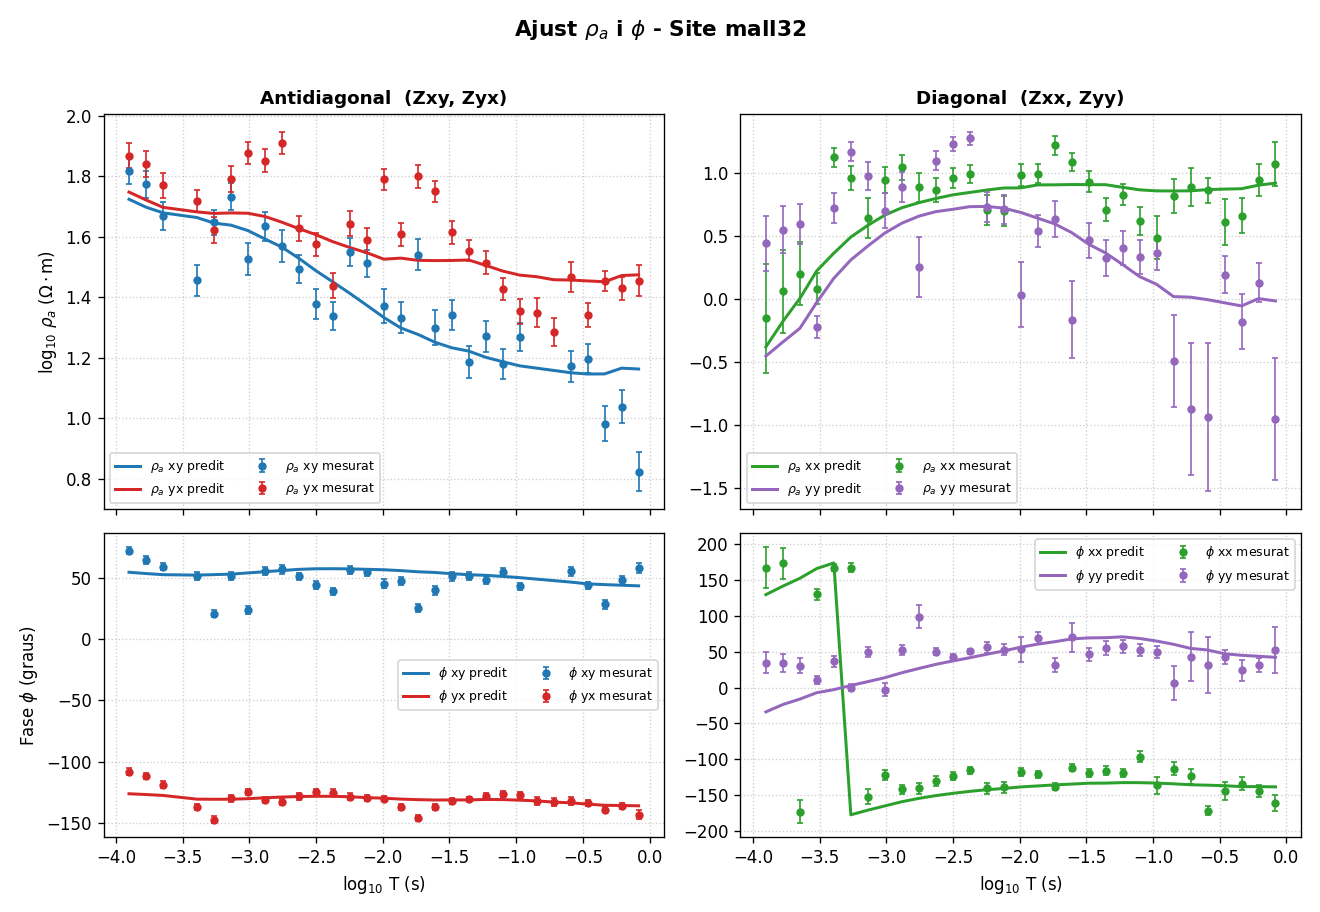
\includegraphics[width=0.198\textwidth]{Ajust_Dades_Fase/mall32f.png} &
    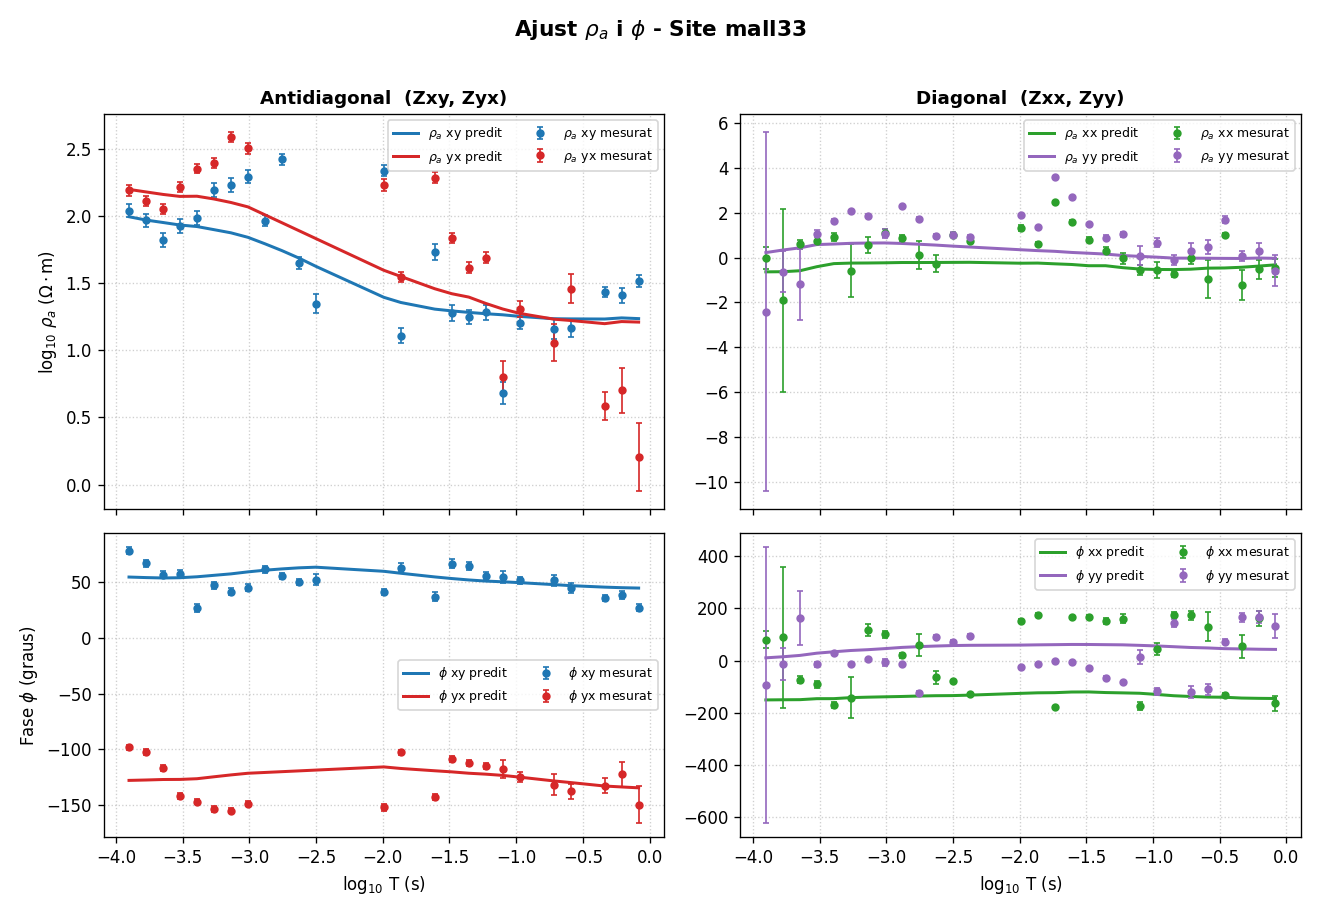
\includegraphics[width=0.198\textwidth]{Ajust_Dades_Fase/mall33f.png} &
    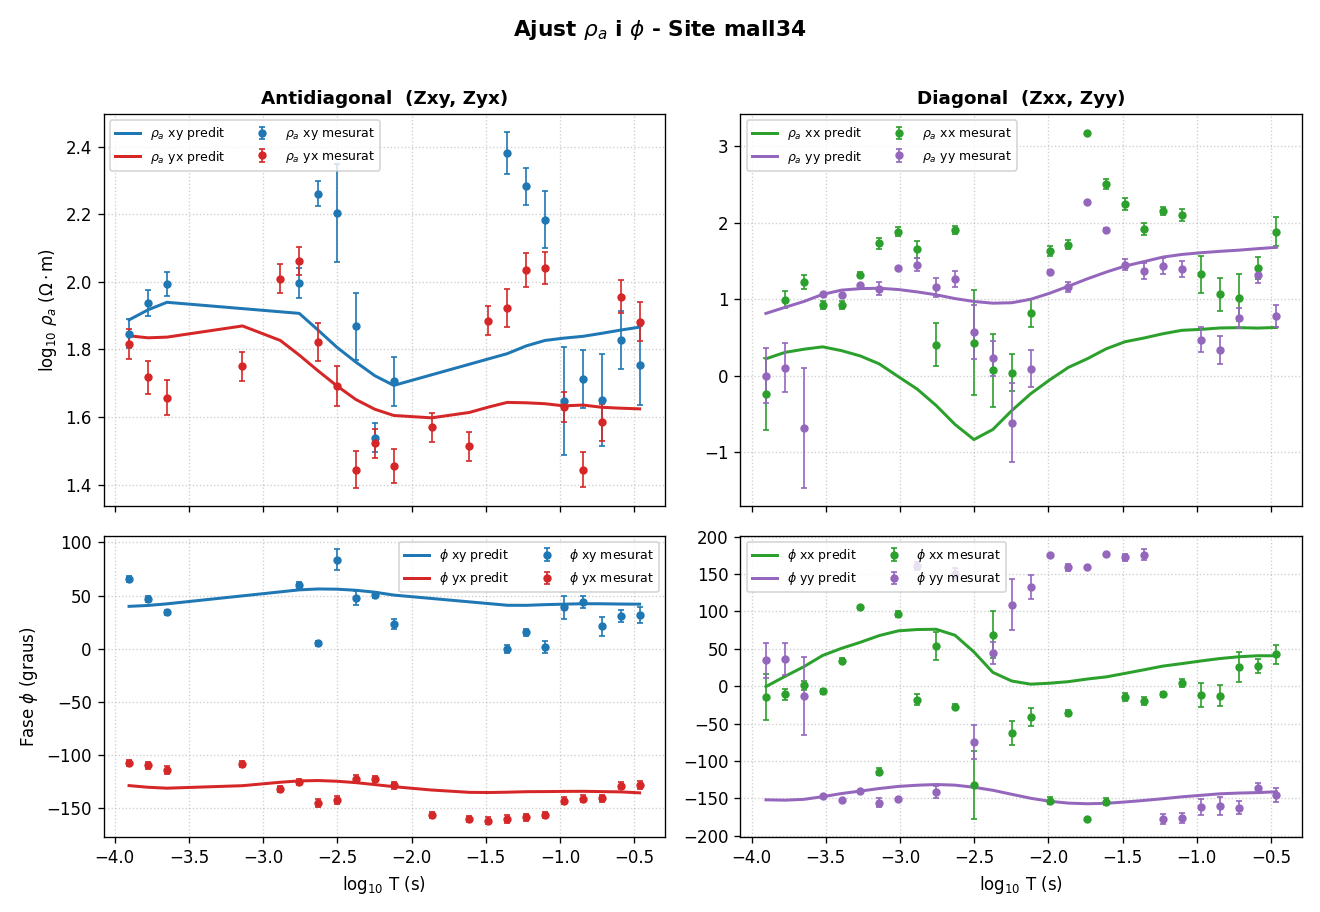
\includegraphics[width=0.198\textwidth]{Ajust_Dades_Fase/mall34f.png} &
    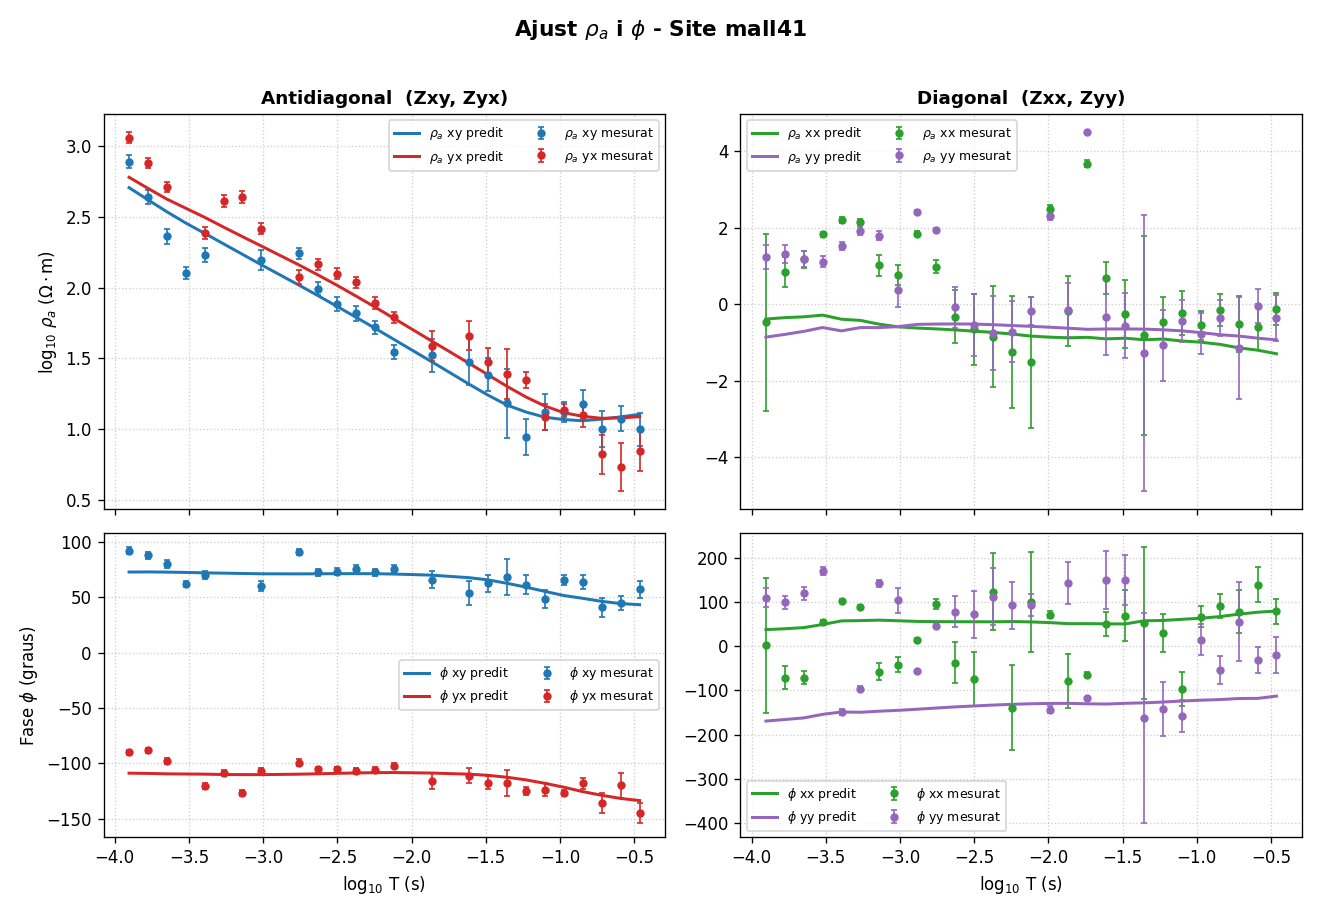
\includegraphics[width=0.198\textwidth]{Ajust_Dades_Fase/mall41f.png} &
    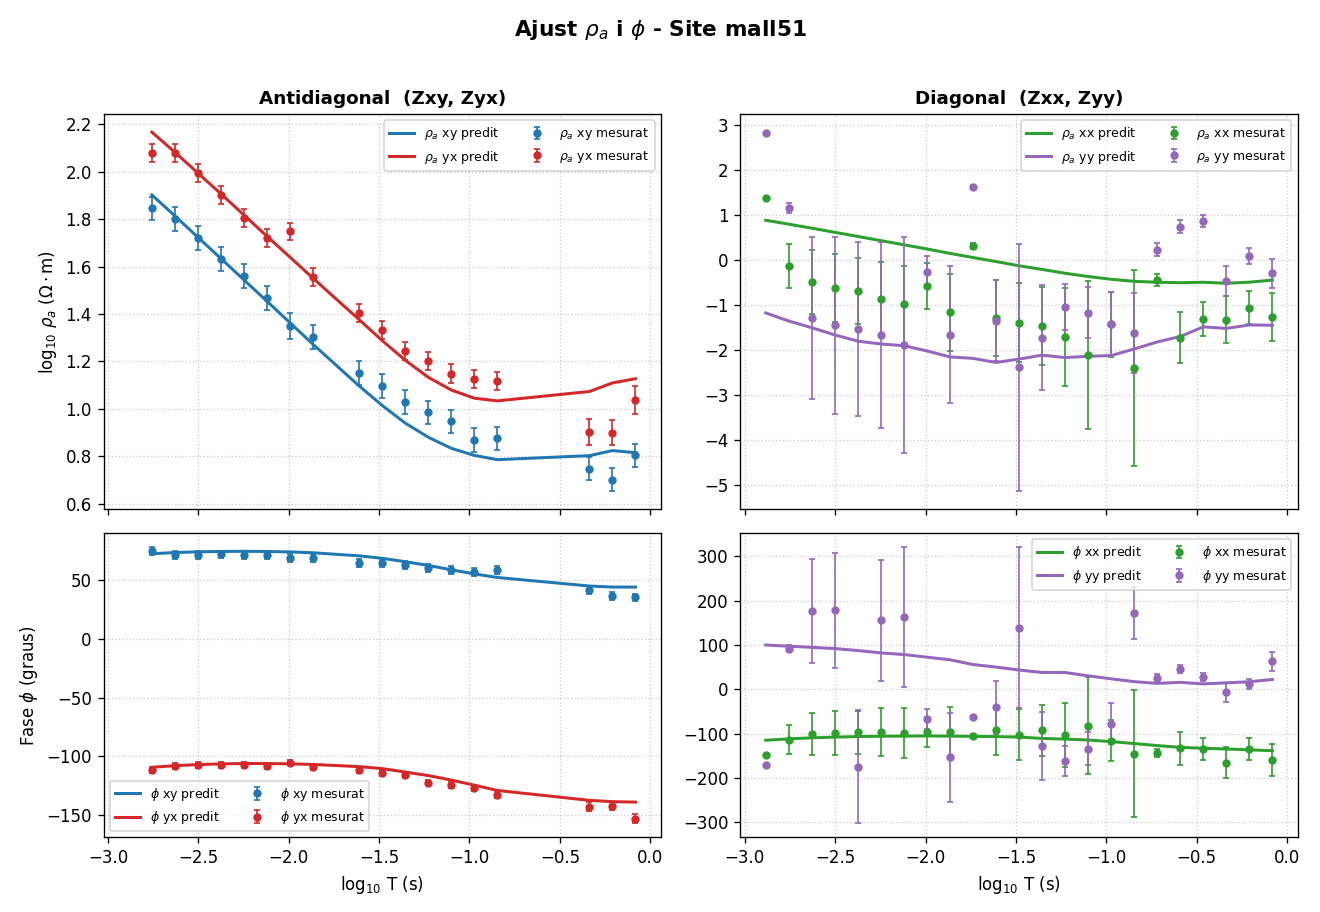
\includegraphics[width=0.198\textwidth]{Ajust_Dades_Fase/mall51f.png} \\[8pt]
    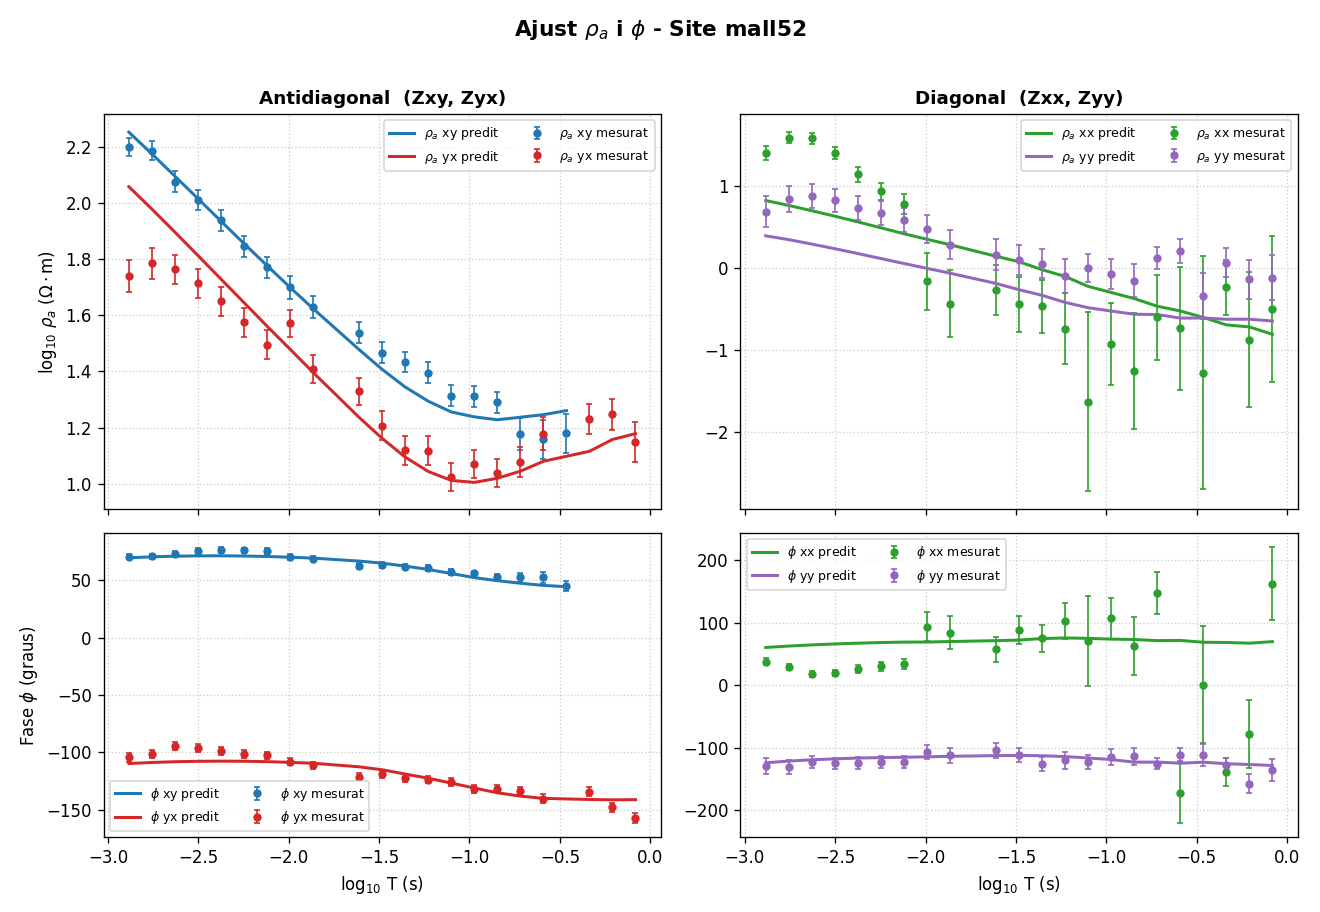
\includegraphics[width=0.198\textwidth]{Ajust_Dades_Fase/mall52f.png} &
    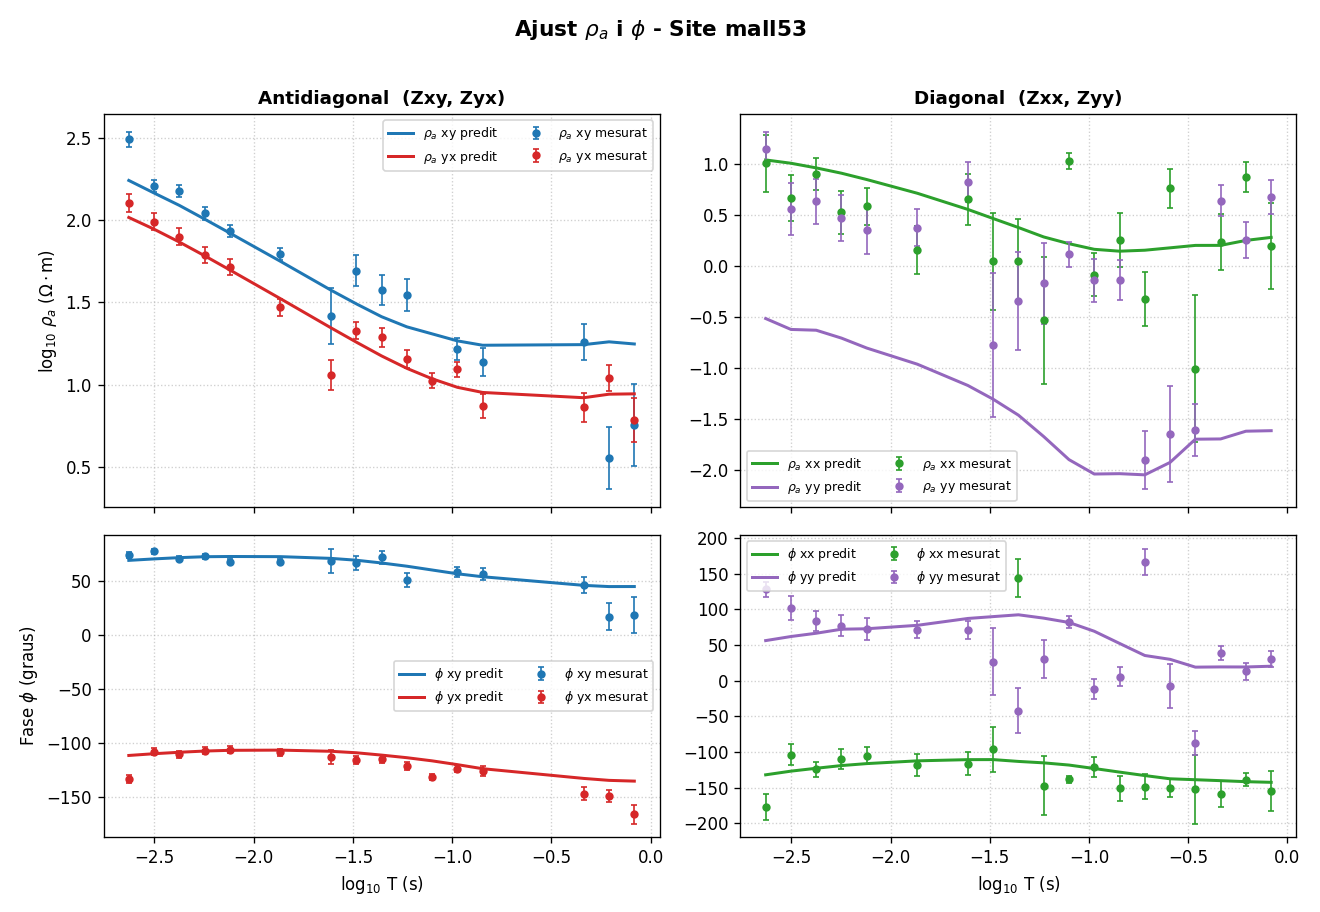
\includegraphics[width=0.198\textwidth]{Ajust_Dades_Fase/mall53f.png} &
    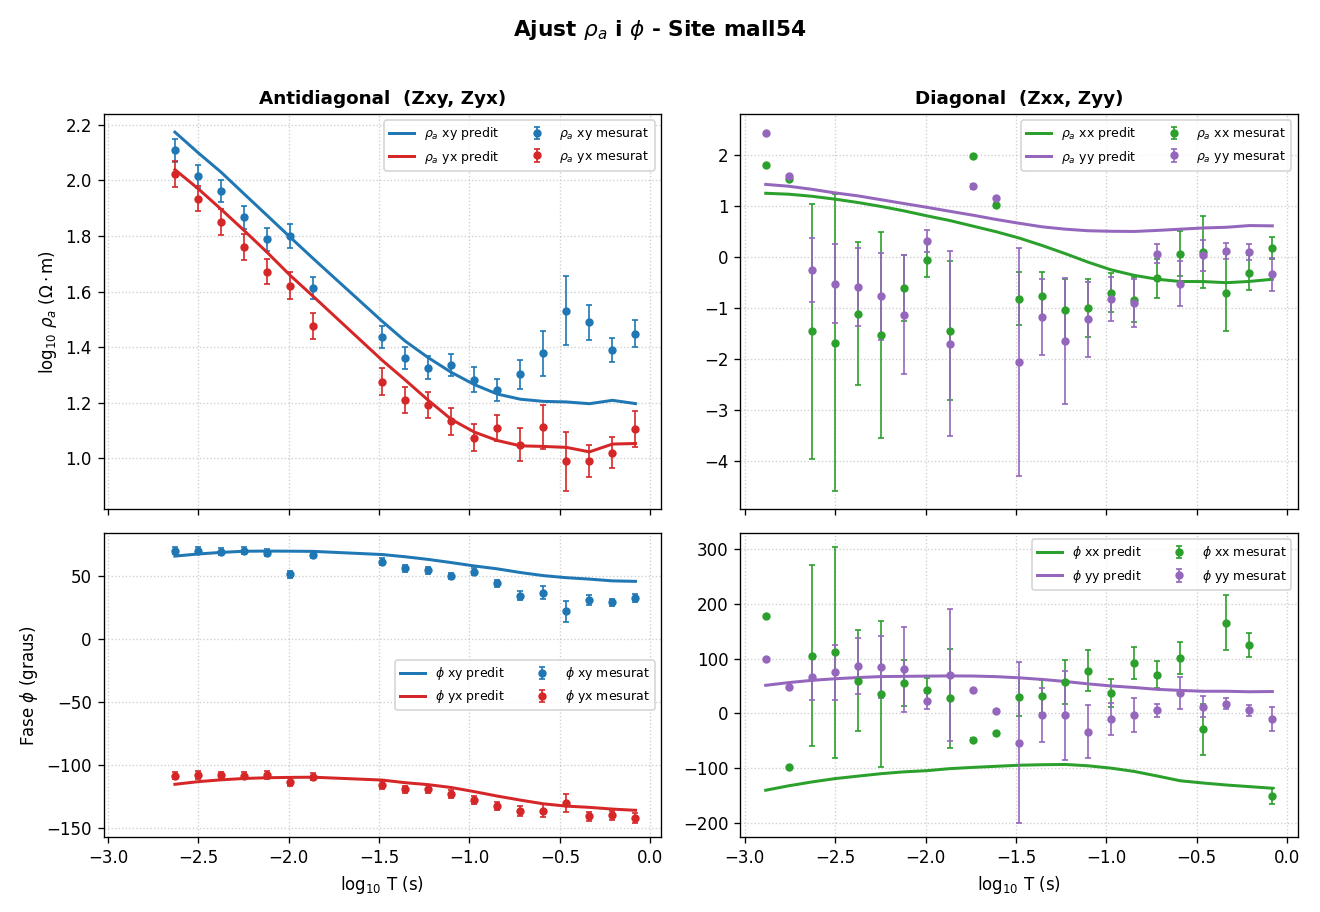
\includegraphics[width=0.198\textwidth]{Ajust_Dades_Fase/mall54f.png} &
    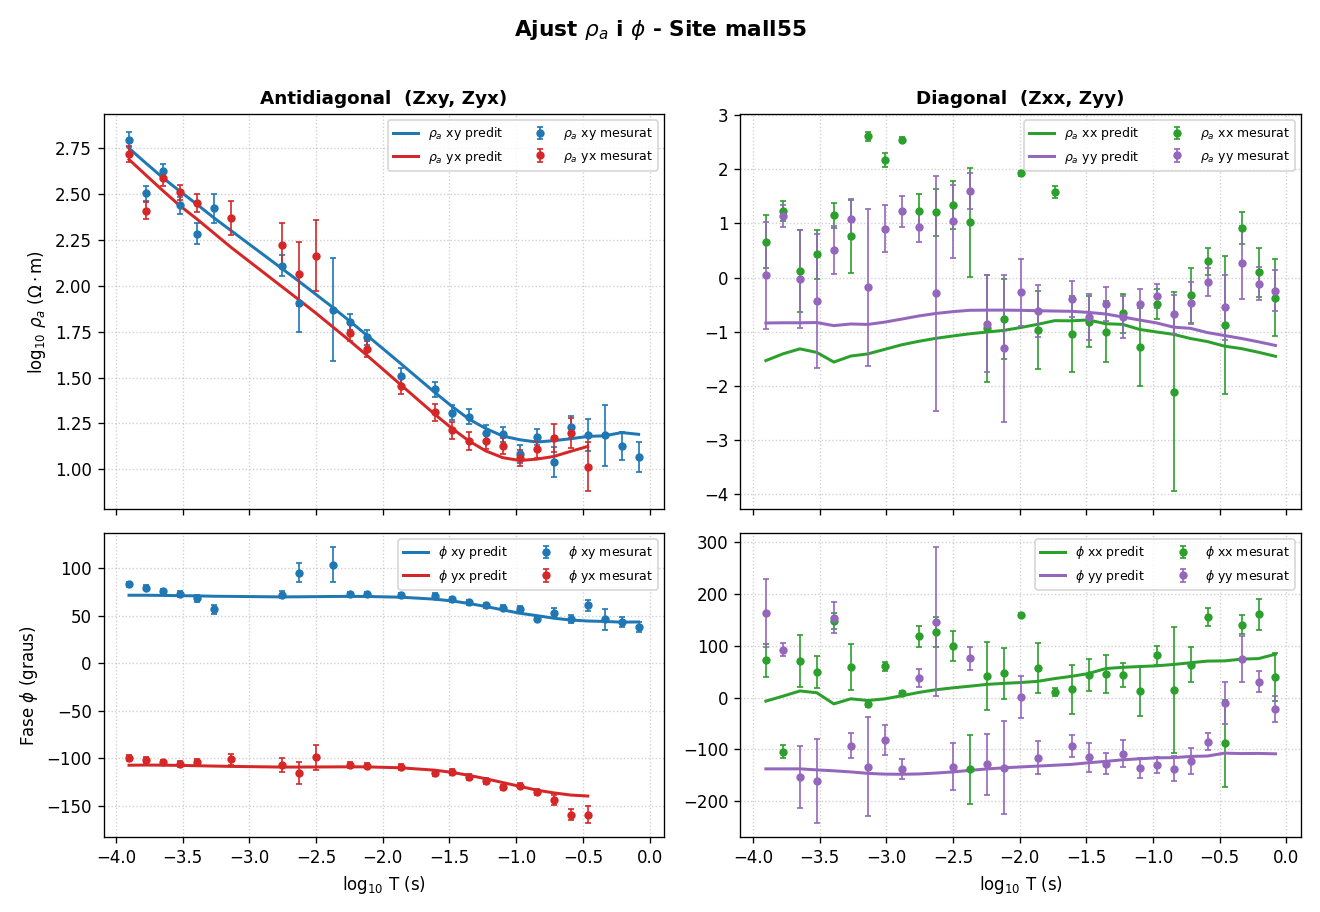
\includegraphics[width=0.198\textwidth]{Ajust_Dades_Fase/mall55f.png} &
    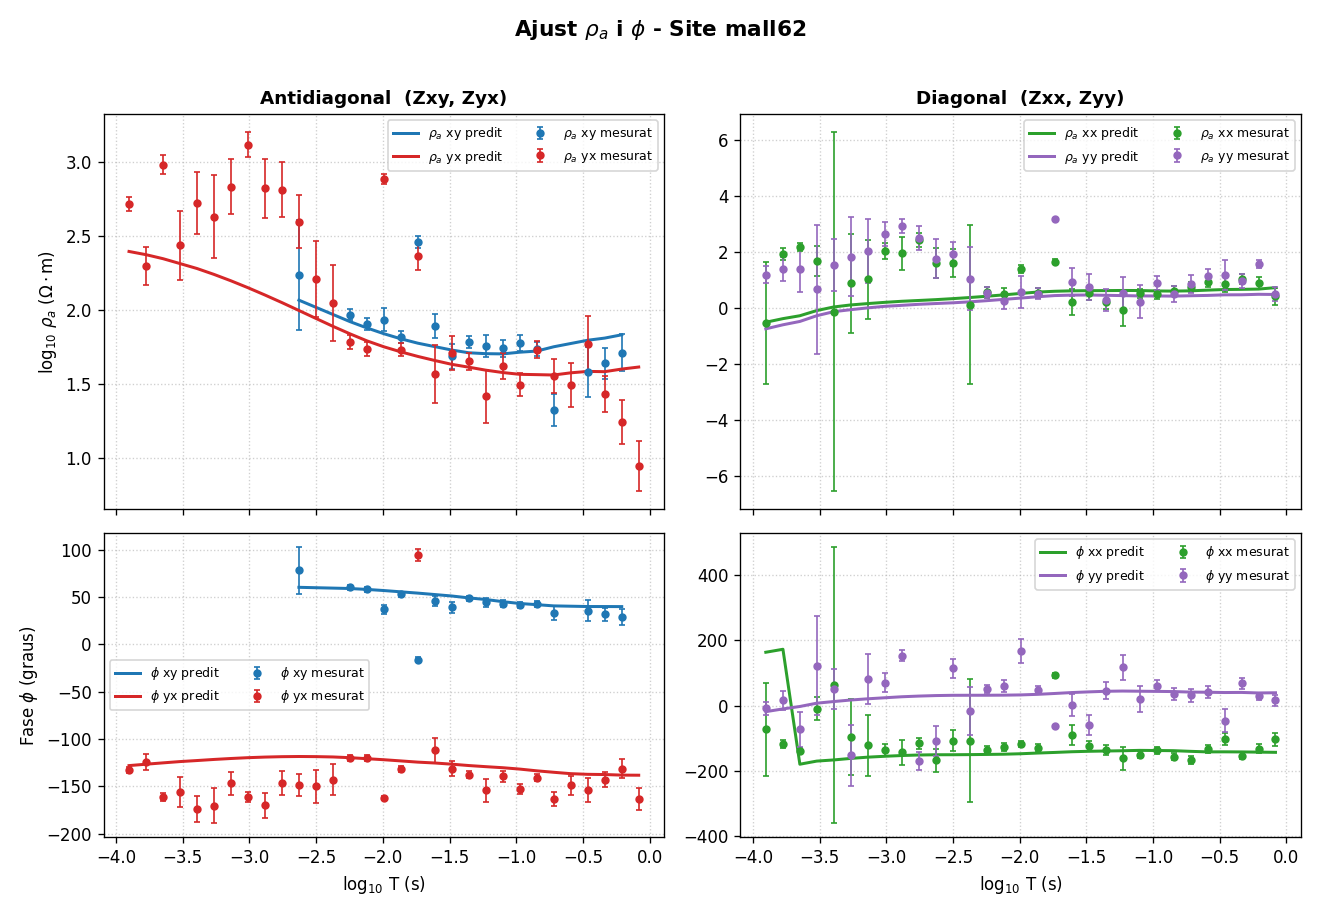
\includegraphics[width=0.198\textwidth]{Ajust_Dades_Fase/mall62f.png} \\[8pt]
    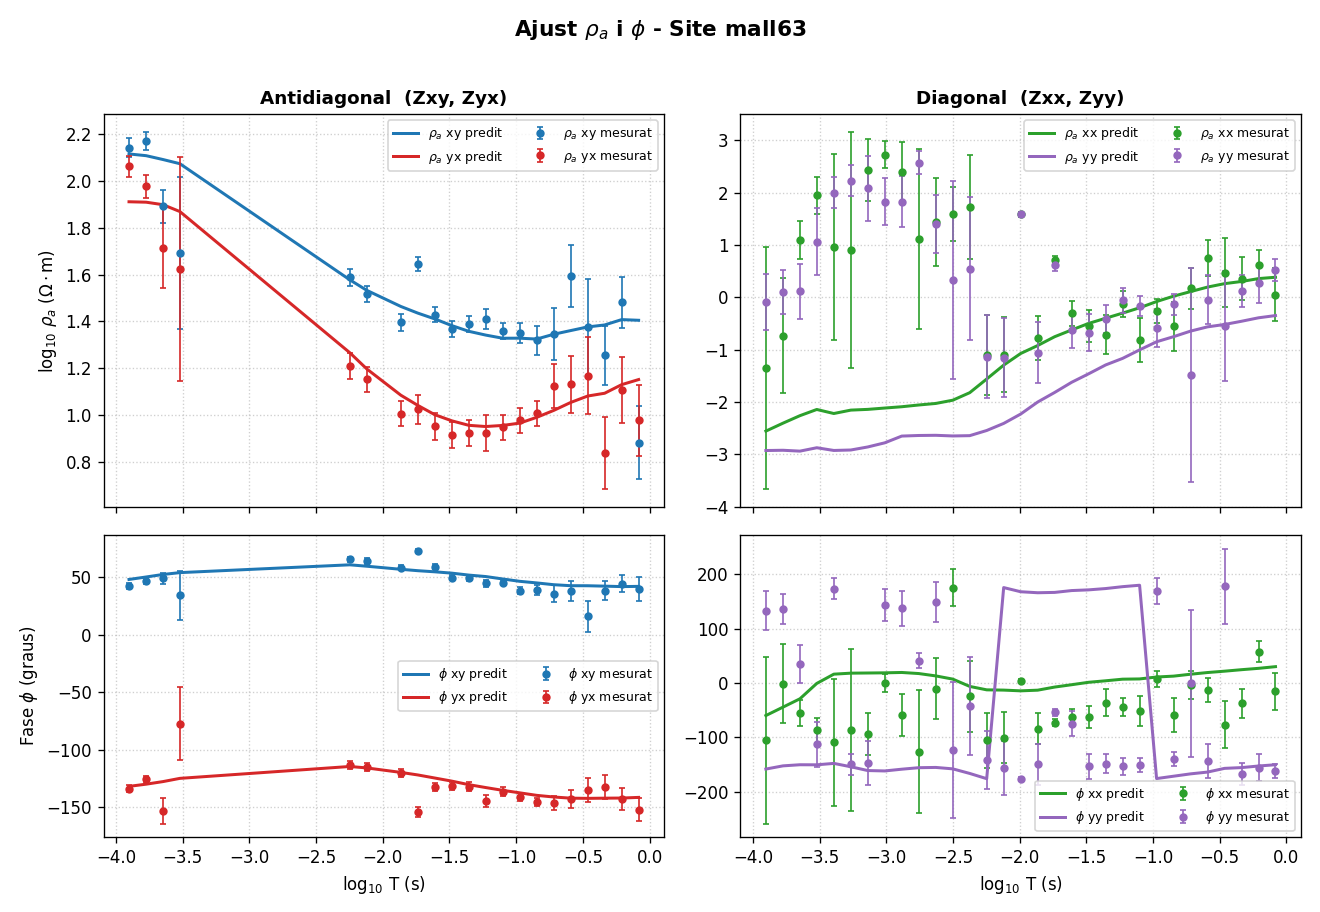
\includegraphics[width=0.198\textwidth]{Ajust_Dades_Fase/mall63f.png} &
    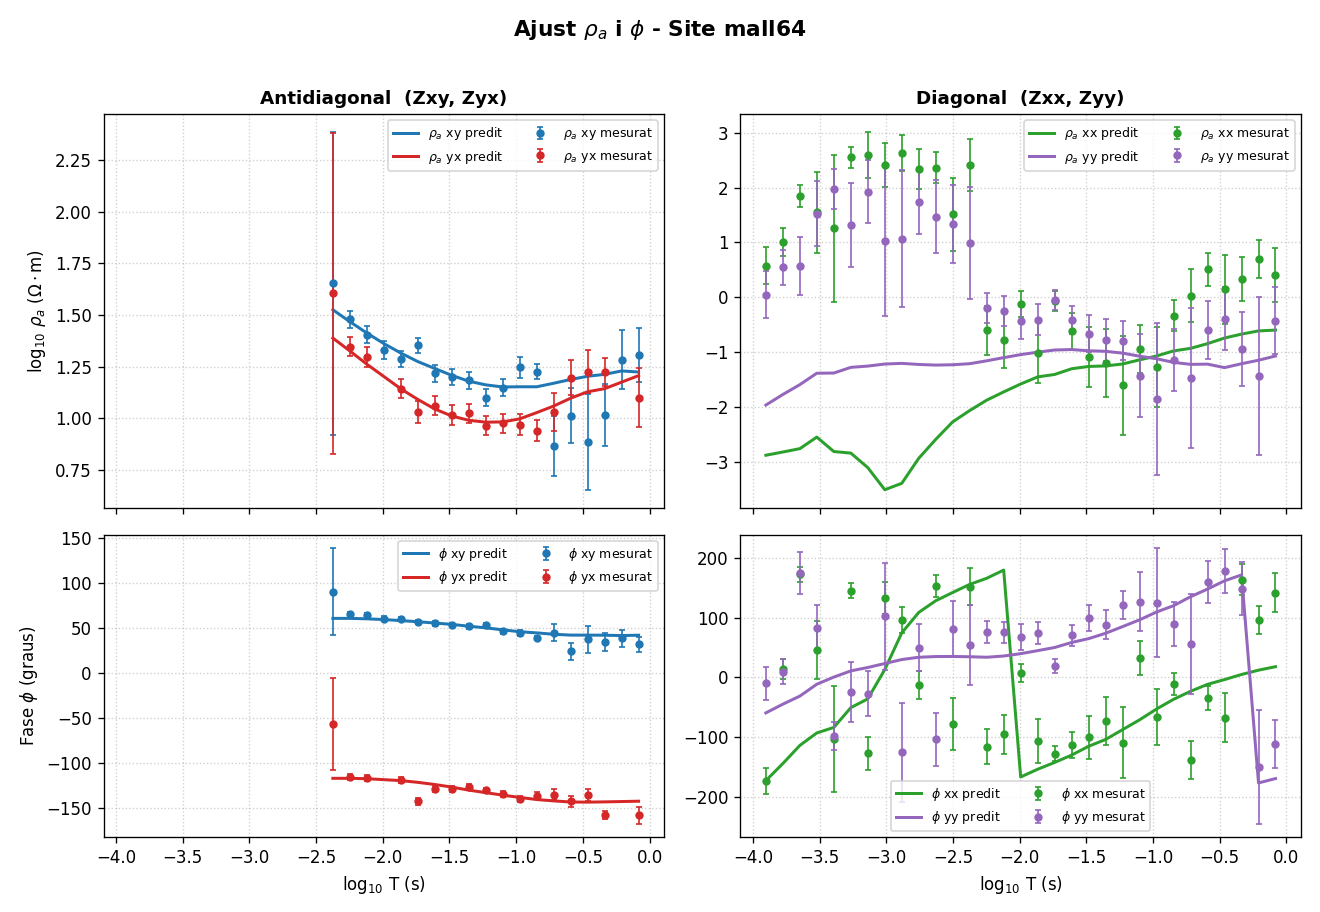
\includegraphics[width=0.198\textwidth]{Ajust_Dades_Fase/mall64f.png} &
    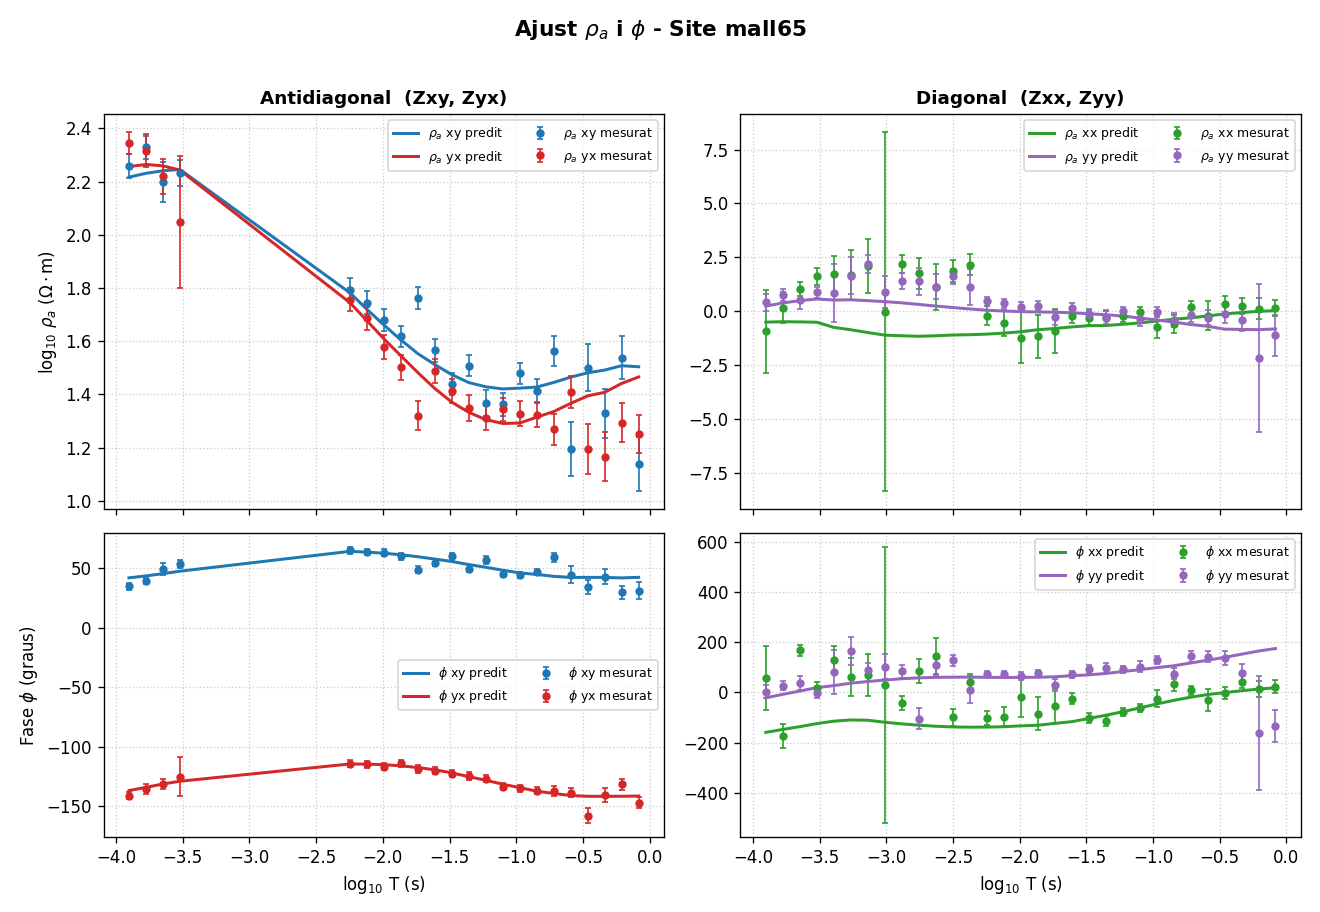
\includegraphics[width=0.198\textwidth]{Ajust_Dades_Fase/mall65f.png} &
    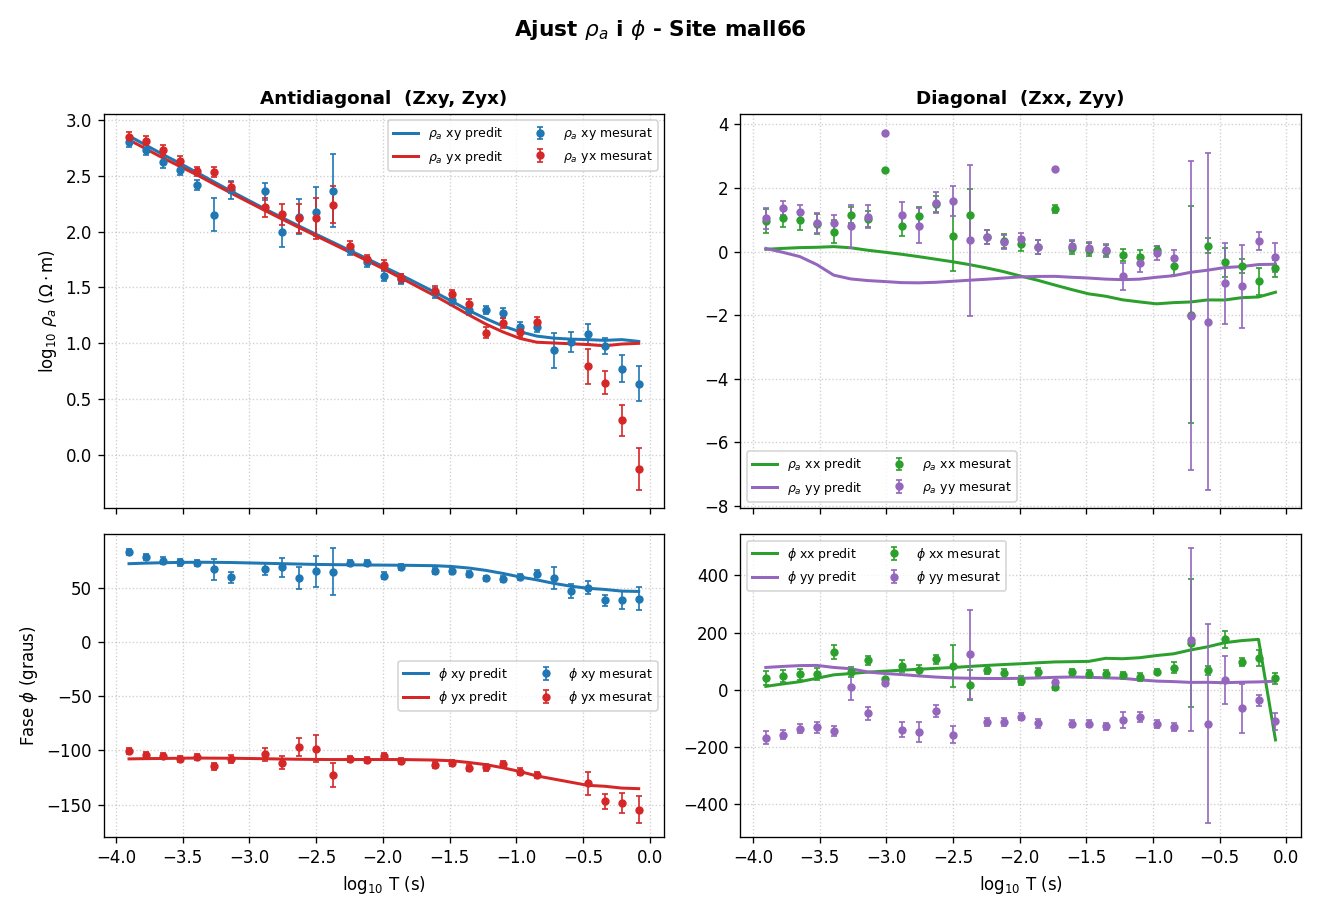
\includegraphics[width=0.198\textwidth]{Ajust_Dades_Fase/mall66f.png} &
    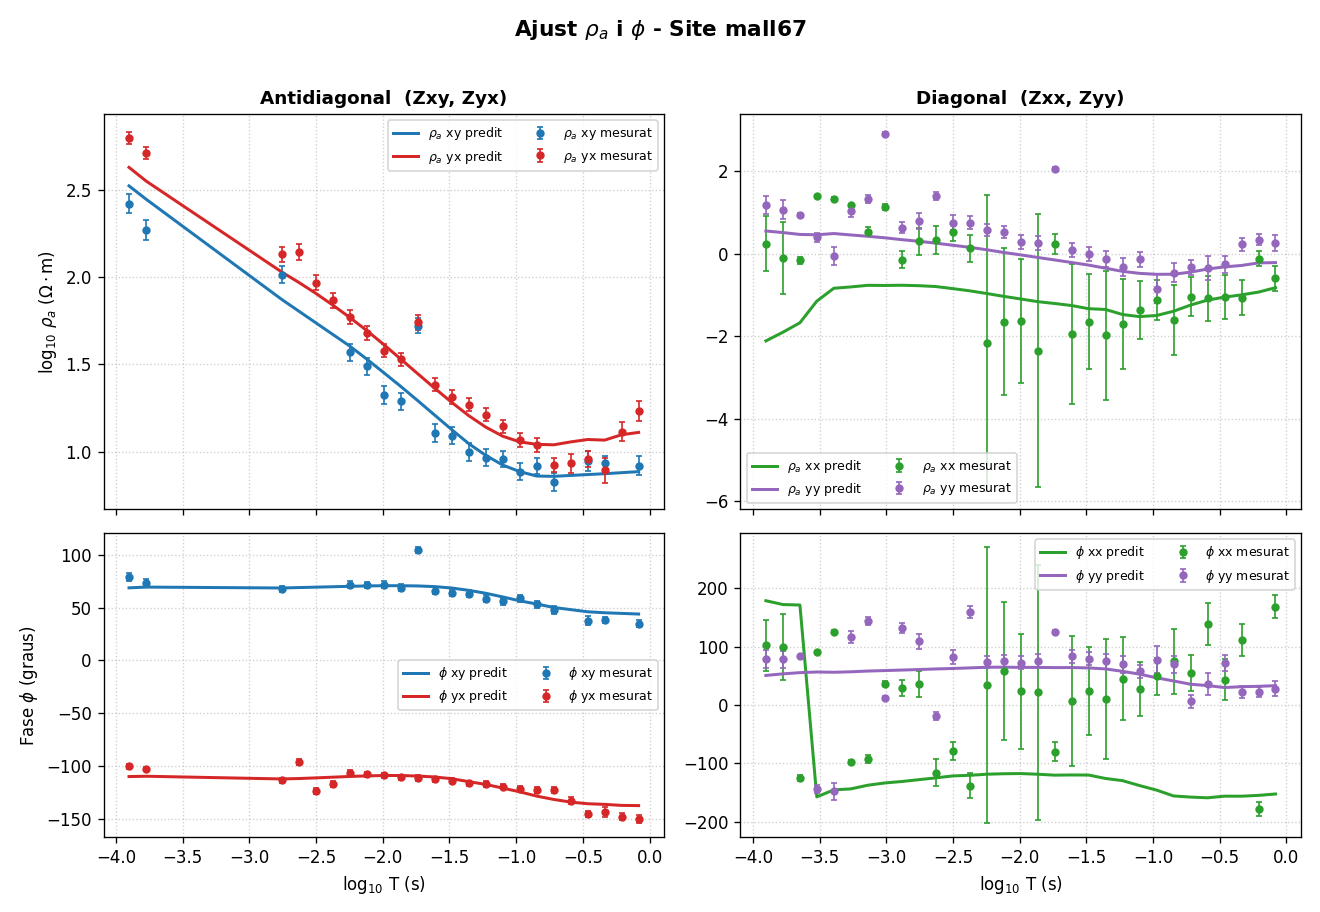
\includegraphics[width=0.198\textwidth]{Ajust_Dades_Fase/mall67f.png}
  \end{tabular}
  \caption{Ajust de la resistivitat aparent i de la fase per a les 40 estacions magnetotel·lúriques.}
  \label{fig:annex-ajust-dades-fase}
\end{figure}
\endgroup

\clearpage

\section{Exemple d'un fitxer EDI}
\label{annex:fitxer-edi}

\begingroup
\setstretch{1}
\noindent
\begin{minipage}[t]{0.49\textwidth}
\lstinputlisting[
    firstline=1,
    lastline=88,
    basicstyle=\ttfamily\fontsize{5.2pt}{6.3pt}\selectfont,
    columns=fullflexible,
    keepspaces=true,
    showstringspaces=false,
    breaklines=true,
    breakatwhitespace=false,
    aboveskip=0pt,
    belowskip=0pt
]{Anex/mall01.edi}
\end{minipage}\hfill
\begin{minipage}[t]{0.49\textwidth}
\lstinputlisting[
    firstline=89,
    lastline=167,
    basicstyle=\ttfamily\fontsize{5.2pt}{6.3pt}\selectfont,
    columns=fullflexible,
    keepspaces=true,
    showstringspaces=false,
    breaklines=true,
    breakatwhitespace=false,
    aboveskip=0pt,
    belowskip=0pt
]{Anex/mall01.edi}
\end{minipage}
\endgroup
\addtocontents{toc}{\protect\endgroup}
\clearpage

\end{document}

%=====================================================================
%  PORTADA OFICIAL INTEGRADA
%---------------------------------------------------------------------
%  El fitxer Portada/Portada-TFG_autoritzacio_CC.pdf s'inclou al
%  començament del document mitjançant el paquet pdfpages.
%=====================================================================
